\documentclass[a4paper,11pt,twoside,openright]{report}
\pdfoptionpdfminorversion=6

\usepackage{graphicx}
\usepackage[ngerman,english]{babel}
\usepackage[utf8x]{inputenc}
\usepackage{fancyvrb}
\usepackage{courier}
\usepackage{helvet}
\usepackage{tikz}
\usepackage{xcolor}
\usepackage{pdfpages}
\usepackage[strict]{changepage}
\usepackage{url}
\usepackage{breakurl}
\usepackage[breaklinks]{hyperref}
\usepackage{amsmath}
\usepackage{marvosym}
\usepackage{hyperref}
\usepackage{caption}
\usepackage{xcolor}
\usepackage{scrextend}
\usepackage{todonotes}
\setlength{\marginparwidth}{2cm}
\usepackage{svg}
\usepackage[font=small,labelfont=bf,margin=\parindent,tableposition=top]{caption}
\usepackage{minted}
\usepackage{subfig}
\usepackage{parcolumns}
\usepackage{floatpag}
\usepackage{natbib}
\usepackage{tcolorbox}
\usepackage{soul}

\newcommand{\todobox}[1]{\begin{tcolorbox}[colback=yellow]#1\end{tcolorbox}}
\DeclareRobustCommand{\hlcyan}[1]{{\sethlcolor{cyan}\hl{#1}}}

%\usepackage[colorlinks=true,linkcolor=blue]{hyperref}%

\def\title{Just-in-time (JIT) compilation for the NEST Simulator to extend the boundaries of neural network sizes on HPC clusters}
\def\author{Benelhedi, Mohamed Ayssar}

\def\UrlBreaks{\do\/\do-}
\hypersetup{colorlinks=true, breaklinks=true,
  linkcolor=black, urlcolor=black, citecolor=black,
  pdftitle=\title, pdfauthor=\author}

% new commands
\newcommand{\source}[1]{\caption*{Source: {#1}} }
\newcommand\todolater[1]{\textcolor{red}{#1}}


% \definecolor{se_dark_blue}{RGB}{0,103,166} % powerpoint
\definecolor{se_dark_blue}{RGB}{0,96,178} % website
% \definecolor{se_light_blue}{RGB}{119,158,201} % powerpoint
\definecolor{se_light_blue}{RGB}{129,160,225} % website


%% setup listings
\usepackage{listings}
\usepackage{xcolor}
\definecolor{codegreen}{rgb}{0,0.6,0}
\lstset{
    numbers=left,
    numberstyle=\tiny,
    numbersep=5pt,
    xleftmargin=11pt,
    xrightmargin=4pt,
    frame=single,
    aboveskip=0pt,
    belowskip=-6pt,
    sensitive=true,
    float=!t,
    breaklines=false,
    captionpos=b,
    tabsize=2,
    showstringspaces=false,
    basicstyle=\small\ttfamily,
    morecomment=[l][\color{codegreen}]{//},
    morecomment=[s][\itshape]{/**}{*/}
}

\definecolor{diffincl}{rgb}{0,0.5,0}
\definecolor{diffrem}{rgb}{0.5,0,0}
\lstdefinelanguage{Pydiff}[]{Python}{%
  morecomment=[f][\bfseries\color{diffincl}]{+\ },
  morecomment=[f][\bfseries\color{diffrem}]{-\ },
}

%% defines the listings laguage named 'MontiArc' derived from the language 'Java' 
%% adding the below listed keywords. See 
%% ftp://ftp.tex.ac.uk/tex-archive/macros/latex/contrib/listings/listings.pdf
%% for listings documentation
\lstdefinelanguage{NESTML}{
 morekeywords={neuron, input, equations, update, state, parameters,end, spike, continuous, real, mV, ms},
}


\definecolor{codegray}{rgb}{0.5,0.5,0.5}
\definecolor{codepurple}{rgb}{0.58,0,0.82}
\definecolor{backcolour}{rgb}{0.95,0.95,0.92}

\lstdefinestyle{jit}{
    backgroundcolor=\color{backcolour},   
    commentstyle=\color{codegreen},
    keywordstyle=\color{magenta},
    numberstyle=\tiny\color{codegray},
    stringstyle=\color{codepurple},
    basicstyle=\ttfamily\footnotesize,
    breakatwhitespace=false,         
    breaklines=true,                 
    captionpos=b,                    
    keepspaces=true,                 
    numbers=left,                    
    numbersep=5pt,                  
    showspaces=false,                
    showstringspaces=false,
    showtabs=false,                  
    tabsize=2
}

\lstdefinestyle{nestml}{
    %backgroundcolor=\color{backcolour},   
    commentstyle=\color{codegreen},
    keywordstyle=\color{magenta},
    numberstyle=\tiny\color{codegray},
    stringstyle=\color{codepurple},
    basicstyle=\ttfamily\footnotesize,
    breakatwhitespace=false,         
    breaklines=true,                 
    captionpos=b,                    
    keepspaces=true,                 
    numbers=left,                    
    numbersep=5pt,                  
    showspaces=false,                
    showstringspaces=false,
    showtabs=false,                  
    tabsize=2
}

\lstset{style=jit}



% Seite einrichten
\setlength{\voffset}{-1in}
\setlength{\hoffset}{-1in}

\setlength{\topmargin}{2.5cm}		   
\setlength{\headheight}{0cm}		   
\setlength{\headsep}{0cm}		   
\setlength{\oddsidemargin}{3,3cm}  % innen ein wenig mehr Rand für die Klebebindung
\setlength{\evensidemargin}{2,7cm} % dafür außen ein wenig weniger
\setlength{\textwidth}{15cm}		   
\setlength{\textheight}{23,5cm}		   
\setlength{\parindent}{0cm}

\newcommand{\emptyLine}{{\LARGE ~\\}}

% tikz set
\usepackage{tikz}
\usetikzlibrary{arrows,shapes,positioning,shadows,trees}
\tikzset{
  basic/.style  = {draw, text width=2cm, drop shadow, font=\sffamily, rectangle},
  root/.style   = {basic, rounded corners=2pt, thin, align=center,
                   fill=red!50},
  level 2/.style = {basic, rounded corners=6pt, thin,align=center, fill=green!40,
                   text width=8em},
  level 3/.style = {basic, thin, align=center, fill=blue!40, text width=10.5em}
}



%caption_setup
\captionsetup{labelfont=bf,labelsep=colon}



\begin{document}

% Einrücken von Absätzen verhindern und 1.5 Zeilen Absatzabstand
\setlength{\parindent}{0pt}
\setlength{\parskip}{1.5ex plus0.5ex minus0.5ex}

\setcounter{tocdepth}{5}
\setcounter{secnumdepth}{5}

% Dieses Teildokument beschreibt die Titelseite.
%

% Seitenzähler auf 1, Römische Ziffern.
\setcounter{page}{1}
\pagenumbering{roman}

\thispagestyle{headings}

%\changepage{<text height>}{<text width>}{<even-side margin>}{<odd-side margin>}{<column sep.>}{<topmargin>}{<headheight>}{<headsep>}{<footskip>}
\changepage{5,1cm}{2.4cm}{}{-0.7cm}{}{-2,3cm}{}{}{}

% Eigentliche Titelseite.
\begin{titlepage}
	
\begin{figure}\raggedleft
\includegraphics[height=3.0cm]{src/pic/logo.jpg}\end{figure}
  
\begin{tikzpicture}[overlay]

% horizontal lines
\draw[color=se_dark_blue, thick] (-1.6, 0.9) -- (17.4, 0.9);
\draw[color=se_light_blue, thick] (-1.4, 0.7) -- (17.4, 0.7);

% vertical lines
\draw[color=se_dark_blue, thick] (-1, 0.9) -- (-1, -24.5);
\draw[color=se_light_blue, thick] (-0.8, 0.7) -- (-0.8, -24.5);

\end{tikzpicture}

\vspace*{-1.5em}

\begin{flushleft}
  {\fontfamily{phv}  
  	{\LARGE
      Rheinisch Westfälische Technische Hochschule Aachen \\
      Lehrstuhl für Software Engineering \\}
    \vspace{3em}
  
    {\LARGE \textbf{\title}\\}
    
    \emptyLine%{\LARGE \textbf{Zweite Titel-Zeile}\\} 
    \emptyLine%{\LARGE \textbf{Dritte Titel-Zeile}\\} % Oder \emptyLine falls nicht Titel kürzer
    \emptyLine%{\LARGE \textbf{Vierte Titel-Zeile}\\} % Oder \emptyLine falls nicht Titel kürzer
    \vspace{3em}
		
    {\Large \textbf{Master Thesis}\\}
		\vspace{3em} 
		
		{\large presented by\\} % presented by
    
    {\LARGE \textbf{\author}\\}
    \vspace{3em} 
		    
  {\Large \textbf{1st Examiner: Prof.\ Dr.\ A.\ Morrison}\\}
    \vspace{1em} 
    {\Large \textbf{2nd Examiner: Prof.\ Dr.\ B.\ Rumpe}\\}
    \vspace{1em} 
    {\Large \textbf{1st Advisor: Charl Linssen}\\}
    \vspace{1em} 
    {\Large \textbf{2nd Advisor: Dr.\ Jochen Martin Eppler}\\}
    \vspace{7em} 
    
% Falls es eine/n zweite/n Betreuer/in gibt, bitte auskommentieren und Namen 
%angeben
%    {\Large \textbf{2. Betreuer:  }\\}
    
   
    
    
    \vspace{7em}

    {\large The present work was submitted to the chair of software engineering \\}
    \vspace{1em}
    % The present work was submitted to the chair of software engineering
		{\large	Aachen, den \today\\}
  }
\end{flushleft}

\end{titlepage}

\changepage{-5,1cm}{-2.4cm}{}{0.7cm}{}{2,3cm}{}{}{}





%%Dieses Teildokument beschreibt die Titelseite.
%

% Seitenzähler auf 1, Römische Ziffern.
\setcounter{page}{1}
\pagenumbering{roman}

\thispagestyle{headings}

%\changepage{<text height>}{<text width>}{<even-side margin>}{<odd-side margin>}{<column sep.>}{<topmargin>}{<headheight>}{<headsep>}{<footskip>}
\changepage{5,1cm}{2.4cm}{}{-0.7cm}{}{-2,3cm}{}{}{}

% Eigentliche Titelseite.
\begin{titlepage}
	
\begin{figure}\raggedleft
\includegraphics[height=3.0cm]{src/pic/logo.jpg}\end{figure}
  
\begin{tikzpicture}[overlay]

% horizontal lines
\draw[color=se_dark_blue, thick] (-1.6, 0.9) -- (17.4, 0.9);
\draw[color=se_light_blue, thick] (-1.4, 0.7) -- (17.4, 0.7);

% vertical lines
\draw[color=se_dark_blue, thick] (-1, 0.9) -- (-1, -24.5);
\draw[color=se_light_blue, thick] (-0.8, 0.7) -- (-0.8, -24.5);

\end{tikzpicture}

\vspace*{-1.5em}

\begin{flushleft}
  {\fontfamily{phv}  
  	{\LARGE
      RWTH Aachen University \\
      Software Engineering Group \\}
    \vspace{3em}
  
    {\LARGE \textbf{First line of title}\\} 
    {\LARGE \textbf{Second line of title}\\} 
    {\LARGE \textbf{Third line of title}\\} % Replace with \emptyLine if title is shorter
    {\LARGE \textbf{Forth line of title}\\} % Replace with \emptyLine if title is shorter
    \vspace{3em}
		
    {\Large \textbf{Bachelor Thesis/Master Thesis/Seminar Paper}\\}
		\vspace{3em} 
		
		{\large presented by\\} 
    
    {\LARGE \textbf{Surname, Prename}\\}
    \vspace{3em} 
		    
    {\Large \textbf{1st Examiner: Prof.\ Dr.\ B.\ Rumpe}\\}
    \vspace{1em} 
    {\Large \textbf{2nd Examiner: }\\}
    \vspace{1em} 
    {\Large \textbf{Advisor: }\\}
    \vspace{7em} 

    {\large The present work was submitted to the Chair of Software Engineering \\}
    \vspace{1em}
    % The present work was submitted to the chair of software engineering
		{\large	Aachen, \today\\}
  }
\end{flushleft}

\end{titlepage}

\changepage{-5,1cm}{-2.4cm}{}{0.7cm}{}{2,3cm}{}{}{}




 % English cover

\clearpage

% Erklaerung

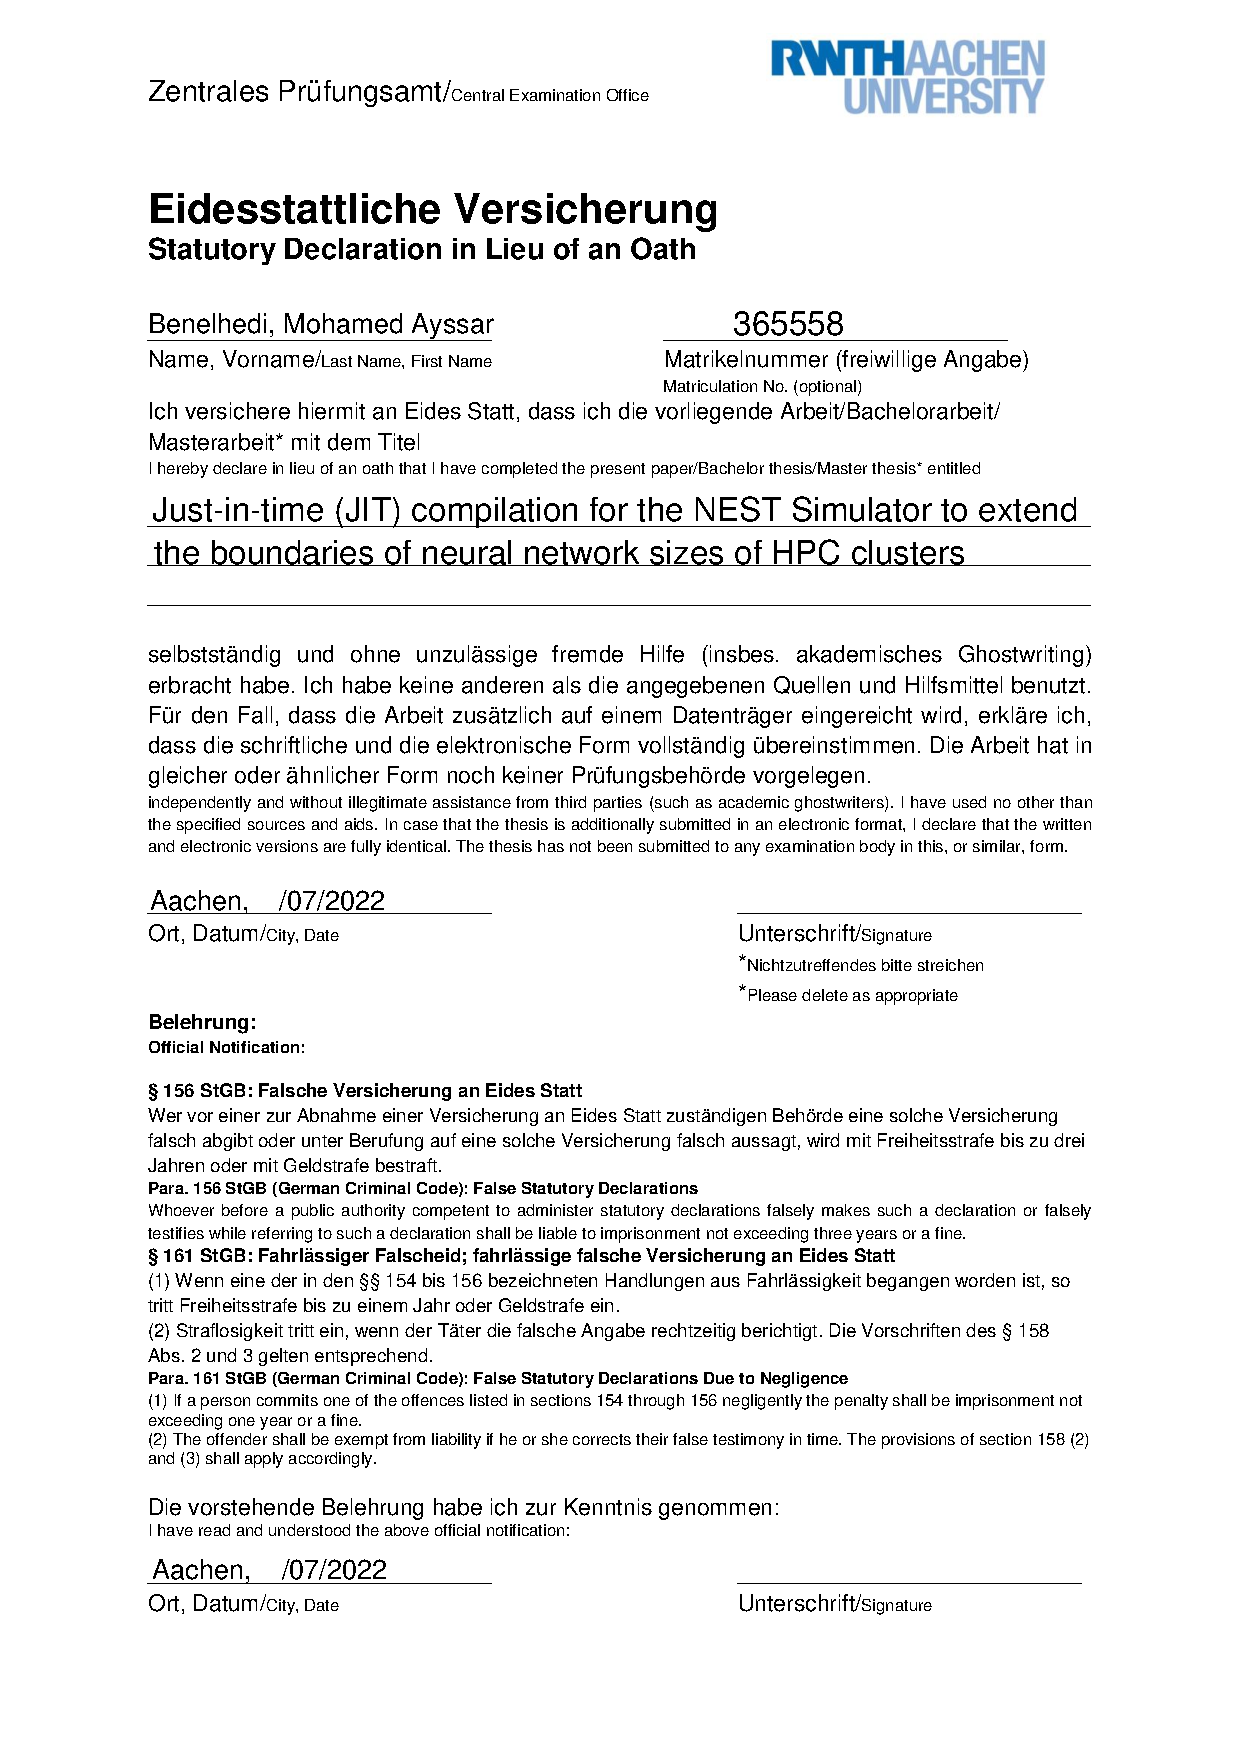
\includepdf[pages={1},offset=-1in -1in]{versicherung.pdf}
% 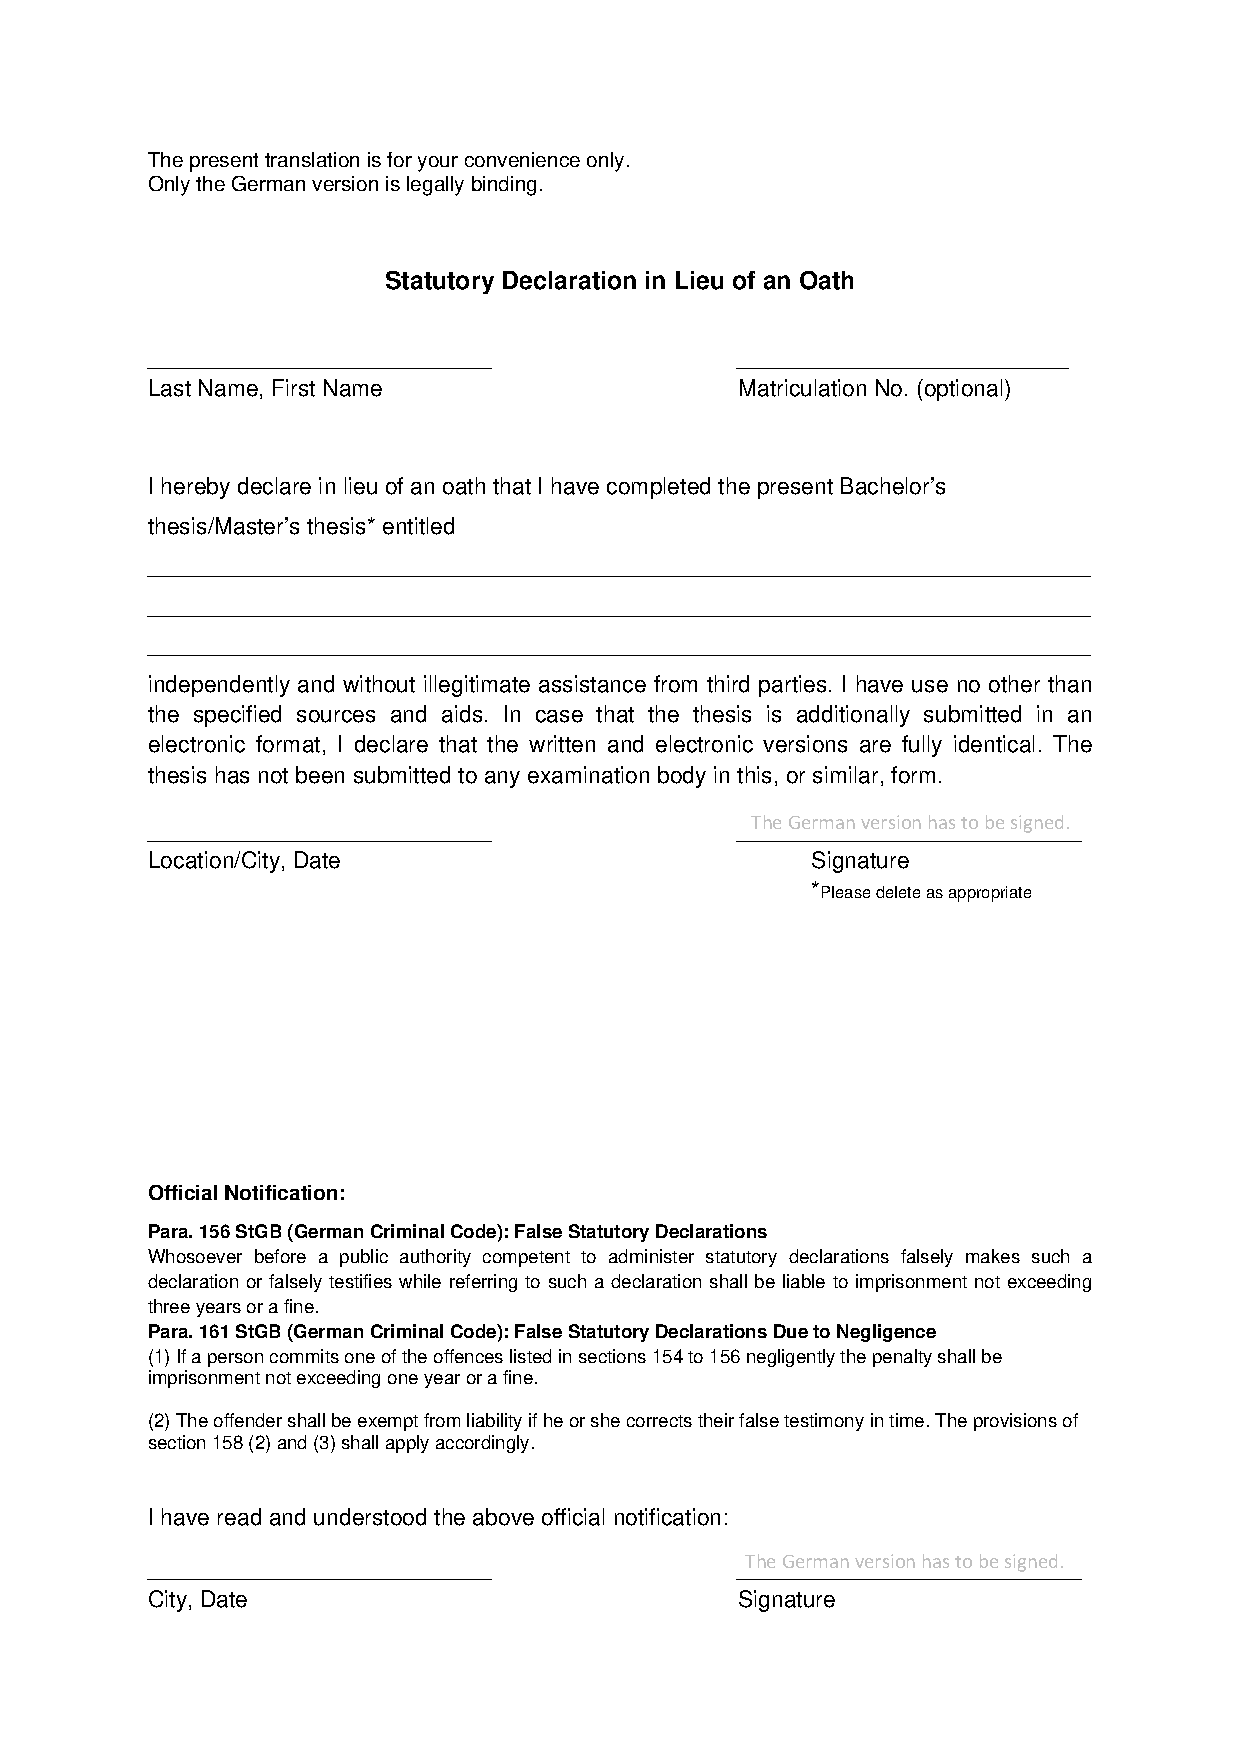
\includepdf[pages={1},offset=-1in -1in]{Statutory_Declaration_in_Lieu_of_an_Oath.pdf} % English 

\clearpage

%\vspace*{2cm}
% Abstract
%{\bf\Large Kurzfassung} \\ [1em] 
%Eine kurze Zusammenfassung der Arbeit.

\begin{abstract}
\emph{NEST} is a simulator for large-scale networks of spiking and non-spiking neural networks \citep{nest}. It profits from both the efficiency of \texttt{C++} and the simplicity of Python to simulate a network with large set of neurons and synaptic connections. Due to the simple interaction between the Python interface (\emph{PyNEST} \citep{10.3389/neuro.11.012.2008}) and the \emph{NestKernel} in C++, users can easily add new models by calling the \texttt{nest.Install()} function within the Python interface. These models are written in C++ and can be loaded dynamically at the runtime.

Fortunately, users don't need to implement their complex models in C++, as they can use \emph{NESTML} \citep{plotnikov2016nestml} to generate the required code given their specification and compile the whole thing into a dynamic library, ready to be used by \emph{PyNEST}. 

\emph{NESTML} is a user-friendly, flexible and a Turing-complete domain-specific language. It simplifies the modeling process for neuroscientists, both with and without prior training in computer science. By specifying the target type, either a different hardware or new supported simulator, the user can still use the same model to generate the code for the given target without any interventions. 

The process of running a simulation script in nest using an external custom model requires providing certain configurations to the \emph{NESTML} code generator. Such configurations cover the model location, model dependency with other models (i.e., custom synapse model) and target platform. Although the \emph{NESTML} code generation is completely automated, the user has to explicitly invoke the \emph{NESTML} interface for the model to be processed and compiled into an extension module for \emph{NEST}, making it usable through calling the \texttt{nest.Install()} function. 

Unfortunately, both the \emph{NEST} and the generated code aren't cache friendly, and they don't fully utilize the single-instruction-multiple-data (\emph{SIMD})\citep{nuzman2006auto}{} execution to increase the performance of the simulation script and all \emph{Object}s in \emph{NestKernel} are stored as an \emph{array of structures (\emph{AoS})}, which might cause a tremendous number of cache misses depending on the size of the network in the simulation.

The goal of the thesis is twofold. Firstly, we eliminate the explicit calls to the \emph{NESTML} interface in the simulation script by \emph{seamlessly} extending the \emph{PyNEST} interface without really making it depends on \emph{NESTML}. This integration allows controlling the logic workflow of the \emph{PyNEST} functions and depending on certain conditions if the model should be instantiated at the given time or delayed and only create the instance  when it is really required. This extension is called \emph{Just-in-time (JIT)} and it refers to the building of the extension module only at the point where it is needed, so instead of invoking \emph{NESTML} upfront, it will be invoked by the \emph{JIT} mechanism when the user
instantiates the neuron (or synapse) using the \emph{PyNEST} call \texttt{nest.Create()} (or \texttt{nest.Connect()}).

The second part focuses on extending the \emph{Nestkernel} to support \emph{Vectorization} by modifying the models. The model becomes the central unit for controlling the state of the nodes instances. Mainly, the vectorized model contains only attributes in the form of \emph{vectors}, and the size of these vectors is the number of instances created during the simulation from that particular model type. Vectorization is introduced in the context of \emph{modularity}, where the model should be decomposed into subcomponents and assembled together during the simulation. 

\emph{Modularity} is what brings \emph{JIT} and \emph{Vectorization} together. During the simulation, by using an external models, the \emph{JIT} is responsible for assembling the components of the model and linking them together, whereas \emph{Vectorization} is responsible for making the components support vectorization and makes sure that linking the components together with the model is done efficiently.

\end{abstract}

\cleardoublepage


%\vspace*{2cm}
{\bf\Large Task Description}

\cleardoublepage


\tableofcontents

\clearpage

% Ab erstem Kapitel Seiten arabisch zählen
\setcounter{page}{1}
\pagenumbering{arabic}
\begin{sloppypar} 
\chapter{Introduction}
\label{chap:intro}

The human body has always been an inspiration for many technologies. Scientists have successfully achieved to understand the mechanics behind different parts of the body and created models that imitate the functionalities of the studied parts. The human brain is one of the most complex organs in the human body \citep{vanderah2020nolte}, and we do still not fully understand its inner workings. Creating machines that can achieve human capabilities such as high-level cognition associated with conscious perception is a human dream since a long time. However, before such a goal can even remotely be achieved, we need to understand how information is processed in the brain, how that would be replicated by machines, and how models of it can be created that target specific functions of the brain and replicate their behavior in connection with other parts of the body.

Due to technical and ethical reasons, neuroscientists may not be able to directly investigate certain parts of the brain and experiment on their responses. Therefore, to avoid experimenting \emph{in vivo} and at the same time attaining realistic results, an embodied simulation framework like presented in \citet{10.3389/fninf.2022.884180} might be used to simulate the brain at scale in order to capture the contributions of multiple brain regions involved in purposeful actions.

Successfully understanding the processes in the brain that create phenomena such as creativity, dreaming and consciousness crucially depends on efficient and easy to use \emph{neural simulators}, the development of which strongly depends on the interaction between researches from both the fields of computer science and neuroscience. Such interactions may lead to a higher quality of the simulation frameworks and as a result to a better understanding of the human mind. One building block in the neural simulation landscape are tools for the creation of neuron and synapse models, which are the basic processing elements of the brain.

\section{Structural and functional units of the nervous system}

The nervous system consists mainly of two types of cells: \emph{neuron} and \emph{glia}. The neurons are information messengers that use electrical impulses and chemical signals to transmit information between different areas of the brain and between the brain and the rest of the nervous system. Everything we \emph{think}, \emph{feel} and \emph{do} would be impossible without the work of neurons. Glial cells provide support for neurons in the form of nutrients and other chemicals and play an important role in keeping the chemical environment of the brain in a good working condition, for example by taking up left-over neurotransmitters or surplus ions from the extracellular space.

\begin{figure}[t!]
  \centering
  \includegraphics[width=0.9\linewidth]{src/pic/neuron.eps}
  \caption{\textbf{The neuron \cite[taken from][]{introductiontopsychology}}. Neurons consist of three major components: The \emph{cell body} (also known as the \emph{soma}) is the core of the neuron containing the nucleus of the cell and responsible for keeping it alive. The \emph{dendrites} are a tree-like, branched structure collecting information from other cells and sending it to the soma. The \emph{axon} is a long-segmented protrusion transmitting information away from the cell body towards other connected neurons. Moreover, some axons are surrounded by a layer of fatty tissue known as the \emph{myelin sheath}. It acts as an insulator and allows faster transmission speeds of the electrical signal by preventing the electrical charge from shorting out.}
  \label{fig:neuron}
\end{figure}

\begin{figure}[t!]
  \centering
  \includegraphics[width=0.9\linewidth]{src/pic/synaptic.eps}
  \caption{\textbf{The synapse \citep[taken from][]{introductiontopsychology}}. Most communication between neurons occurs at specialized structures called \emph{synapses}. The synapse is the area where two neurons come close enough that they are able to pass a chemical signal (\emph{neurotransmitters}) from one to another. The gap between the neurons where this chemical exchange takes place is called the synaptic cleft. Neurotransmitters are packaged into small sacs called vesicles (blue circles in the figure). Each vesicle can contain thousands of neurotransmitter molecules. When the pre-synaptic neuron gets active, this causes the vesicles to fuse with the pre-synaptic membrane and release the neurotransmitter molecules into the cleft. Once the neurotransmitter are in the synaptic cleft, they interact with the receptors on the post-synaptic membrane, bind with them, and may cause an action to occur in the post-synaptic cell.}
  \label{fig:synapse}
\end{figure}

The whole process of communication between neurons (depicted in \autoref{fig:neuron}) is based on passing an \emph{electrochemical} signal from one neuron (called the \emph{pre-synaptic} neuron) to many neurons (called \emph{post-synaptic} neurons). A received electrical impulse travels through the neuron and a chemical reaction is triggered to transmit the signal to the next neuron. When a signal is received at the level of the \emph{dendrites}, it is transmitted to the \emph{soma} in the form of an electrical signal. If the accumulated signal is strong enough, it may be forwarded to the axon and afterwards to the synapses. Reaching these terminal stations, a chemical reaction takes place, emitting \emph{neurotransmitters}, which are transported to connected neurons across the space between the cells. See \autoref{fig:synapse} for details.

We distinguish three states (or phases) that a neuron can undergo, the \emph{resting state}, the \emph{action potential} and the \emph{hyper-polarization} as depicted in \autoref{fig:action_potential}. In the \emph{resting state}, the interior of the cell contains a greater number of negatively charged ions than the outside of the cell. This imbalance leads to a measurable \emph{membrane potential} of about -55 mV. If the first segment of the axon is stimulated by an incoming signal travelling down from the \emph{dendrites} and if the impulse is strong enough to reach a certain \emph{threshold}, the segment opens its voltage-gated ion-channels, allowing positively charged sodium ions (Na+) to enter. This change in electrical charges is known as an \emph{action potential} or \emph{spike} due to the form of the excursion of the membrane potential. Once an action potential is elicited, the number of positively charged ions exceeds the number of negative ions in the segment, and it becomes temporarily positively charged. As a consequence, a similar electrical change occurs in the next segment, allowing the electrical impulse to travel along the axon as a wave until it reaches the synapses. It is important to note here that when the signal passes the next segment, the prior segment's gates close again and the potential returns to its original state.

\begin{figure}[ht!]
  \centering
  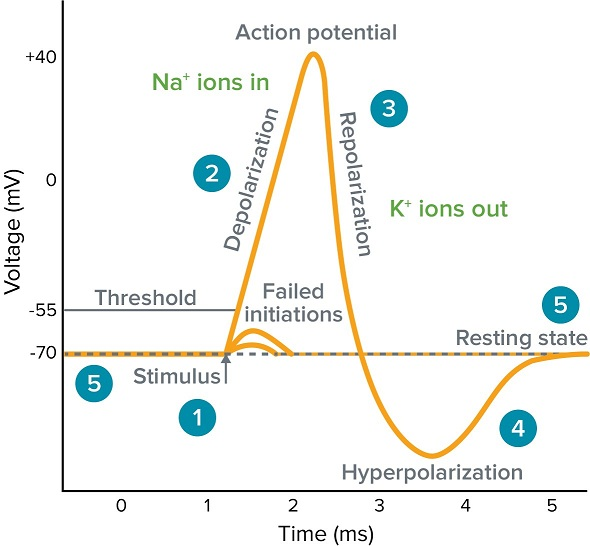
\includegraphics[width=.5\linewidth]{src/pic/what-is-action-potential.jpg}
  \caption{\textbf{The action potential \citep[taken from][]{what-action-potential}}: (1) A stimulus triggers a rapid change in the membrane potential, called an action potential (or, due to the shape of the excursion, spike). A sufficient current must be accumulated in the cell in order to raise the voltage above the threshold to start a membrane depolarization. (2) Depolarization is depicted as the rising phase, and it occurs when the sodium channels in the cellular membrane open, causing a large influx of sodium ions. (3) Membrane repolarization results from rapid sodium channel inactivation as well as a large efflux of potassium ions resulting from activated potassium channels. (4) Hyperpolarization is a lowered membrane potential caused by the efflux of potassium ions and closing of the potassium channels. (5) Resting state is when membrane potential returns to its resting voltage before being stimulated.}
  \label{fig:action_potential}
\end{figure}


An important property of the action potential is that it cannot be partial. It is that the neuron either \emph{fires} completely, such that the action potential travels all the way down the axon, or it does not fire at all. After firing a spike, the neuron is not able to instantly fire again due to the depletion of its neurotransmitter vesicles. This is true even if other electrical impulses are being accumulated at the dendrites. This period of \emph{hyper-polarization} is also called the \emph{refractory period} of the neuron.

When an axonal action potential reaches the terminal stations, the electrical impulse signals them to release neurotransmitters into the synaptic cleft. These neurotransmitters travel across the synaptic space between the terminal stations of one neuron and the dendrites of the others, where they bind to specific receptors. Neurons may have the property of either having an \emph{excitatory} or \emph{inhibitory} effect to their post-synaptic neurons. Excitatory neurotransmitters increase the neuron's likelihood to fire, while inhibitory neurotransmitters decrease the cell's likelihood to fire. Given that different neurotransmitters arrive at the dendrites, the neuron will be influenced by both excitatory and inhibitory signals. The neuron accumulates both types of signals and when the total effect of the excitatory signals are greater than the total effect of the inhibitory signals, the neuron moves closer to its signal transduction threshold. Reaching the threshold, the signal is transmitted via the dendrite and the process begins anew in the next cell.

The efficacy of a synapse between a pre-synaptic and a post-synaptic neuron may change over time and depending on the intensity of the activity transmitted via it, the synapse might either get stronger, weaker, or be removed completely. These changes are subsumed under the term \emph{synaptic plasticity}. The synaptic strength depends on how often the two neurons communicate, and may change on short or long timescales. Short-term synaptic plasticity refers to the temporal change in the synaptic strength as a form of adaptation to continued activity, and wears off over minutes or hours. In contrast to this, the long-term synaptic plasticity may last for hours, days or even years and is responsible for storing new information in the brain and thus forms the basis for forming memories and learning.

\section{Neuronal simulation}

A cubic millimeter of mouse cortex contains about $9×10^4$ neurons and $7×10^8$ synapses \citep{faisal2005ion}. This tremendous number of neurons and connections makes it hard to conquer the overall complexity of the brain. Computer simulations can be a helping tool, but they have to be very efficient in simulating the targeted parts and representing the available resources.

A neural simulator is a piece of software that allows the user to specify the behaviour of models in a high level language, in mathematical notation, or directly as a computer implementation. To be of maximal use, simulators should implement computationally efficient algorithms and support large-scale modelling and complex biophysical models. In order to minimize the entry barrier and reduce the development time, simulators should come with easy to use user interfaces. Examples for neuronal simulators on the level of single neurons and synapses are NEST \citep{gewaltig2007nest} and Brian \citep{10.3389/neuro.11.005.2008}. Both handle connectivity of the neurons as a graph $\mathcal{G}$ \citep{bondy1976graph}, with neurons being the set of nodes $\mathcal{V}$ and synapse as the connections between the nodes $\mathcal{E}$. Neurons and synapses in both these simulators replicate different properties of their biological counterparts.

The same graph $\mathcal{G}$ may have different interpretations depending on the abstraction level. The nodes in the graph may represent the interaction of molecules inside the cells, and it is known as the \emph{reaction diffusion} model. The \emph{population} model is another interpretation of the graph $\mathcal{G}$ that aggregates different neurons in one region and analyses the interaction between the regions. The \emph{point neuron} model is similar to the population model, with the single different that the nodes in the graph are the single neurons and not the grouped regions. Building simulators that can recreate the same behaviour based on these interpretations might be a hard problem, as these abstractions might either require a lot of resources, or they are so complex in the structure that we can not compute the interaction of the nodes with each other.


For this thesis, NEST was chosen as the platform to test the developed ideas and implementations, as it is an open source tool and has a well-structured and modern architecture. The basic concepts are however general and could in principle be ported to other simulators than NEST.

The \emph{neural simulation tool NEST} \citep{gewaltig2007nest, spreizer_sebastian_2022_6368024} is capable of simulating large neuronal networks with different neuron and synapse models. NEST is written in C++ and employs OpenMP for in-node parallelization using threads and the message passing-interface MPI \citep{clarke1994mpi} for distributed simulations. Its Python interface \citep[\emph{PyNEST};][]{10.3389/neuro.11.012.2008} makes it easy for users to run the simulations. Neuron models may be anything from simple \emph{point neurons} like the \emph{integrate-and-fire} neuron to more complex compartmental neurons. While synapses may either be \emph{static} or have a variant weight that changes over time according to a \emph{plasticity} algorithm. NEST supports a variety of algorithms for synaptic plasticity. Examples for such algorithms are spike-timing-dependent plasticity (STDP), short-term plasticity (STP), or third-factor neuromodulated weight dynamics.

The neural network in NEST is generated from neurons and their connections using high-level API functions in PyNEST. The most essential functions are \texttt{Create()}, which is responsible for creating instances of the desired neuron models, \texttt{Connect()}, which connects the neurons and shapes the topology of the neural network, and \texttt{Simulate()}, which drives the state of the dynamic system in time. The type of the synapse model used between the pre-synaptic neuron and the post-synaptic neuron is defined in the \texttt{Connect()} function. \autoref{lst:simple_simulation} shows a simple example of how to create two neurons and connect them using a specific synapse type and run the simulation.\\

\begin{figure}[ht!]
  \centering
\begin{lstlisting}[language=Python, label=lst:simple_simulation, caption={Every simulation script using PyNEST starts with importing the \texttt{nest} module in Python. In line 4, we create two Hodgkin-Huxley neurons as instances of the \emph{hh\_psc\_alpha\_gap} model. In line 5, we set a background current of 100.0 pA for both neurons. Line 6 modifies the initial membrane potentials of the first neuron instance to be at -10.0 mV. In line 8, we create a \texttt{voltmeter} to record the membrane potential of both neurons. In line 11, we connect the first neuron with the second neuron, and vice-versa using the \emph{gap\_junction} synapse model. Finally, we connect the voltmeter to the neurons to record their membrane potential over the course of the simulation in line 15 and run the simulation for 10.0 milliseconds in the last line by calling \texttt{Simulate()}.}, captionpos=b]
import nest

# Create neurons and devices
neurons = nest.Create('hh_psc_alpha_gap', 2)
neurons.I_e = 100.0
neurons[0].V_m = -10.0

vm = nest.Create('voltmeter', params={'interval': 0.1})

# Connect neurons and devices
nest.Connect(neurons, neurons,
    {'rule': 'all_to_all', 'allow_autapses': False},
    {'synapse_model': 'gap_junction', 'weight': 0.5})

nest.Connect(vm, neurons, 'all_to_all')

# Simulate the neural network
nest.Simulate(10.0)
\end{lstlisting}
  %\caption{The Simulation script imports without \emph{JIT}}
  %\label{fig:imports_without_jit}
\end{figure}

Being a research tool, NEST is constantly applied to new use cases, and the set of built-in neuron and synapse models is by definition never complete. In order to not restrict users to only the models that come with NEST, they can create custom neuron and synapse models with the NEST Modelling Language \emph{NESTML} \citep{plotnikov2016nestml, linssen_charl_a_p_2022_5784175}. NESTML allows users to express models by specifying their state variables, parameters, equations, and optionally a procedural description of the state update. Such models can then be used in simulation studies by loading the generated and compiled model libraries at runtime into NEST.

NESTML itself is written in Python and consists of two parts: The first is a language specification that is heavily based on the syntax of Python, but also provides domain concepts like physical units and differential equation as first class concepts. Each custom model in NESTML is defined by its name in the \emph{neuron} block of the language, and the specified name is used for generating the library code in C++ and for using the model in the simulation script. The second part of NESTML is a tool chain that takes a model description and produces C++ code and the boilerplate code required to compile the model into a dynamically loadable library. The most important function in the Python interface to NESTML (\emph{PyNESTML}) is the function \texttt{generate\_nest\_target()}, which generates an extension module for NEST given one or more \texttt{.nestml} files. After installing the library, instances of the model can be created using PyNEST's \texttt{Create()} function and connected with other elements in the network using the \texttt{Connect()} function.

\vspace{2em}
\begin{figure}[ht!]
\centering
\begin{lstlisting}[language=Python, label=lst:nestml_without_synapse, caption={Generating extension module code: The \texttt{generate\_nest\_target()} call for only a neuron model. The minimum required parameter of the function is the \texttt{input\_path} that points to the location of the model. Once the code is generated, the built libraries can be loaded into NEST using the \texttt{Install} function by providing the name of the module (\emph{simple\_module}). Once the model is installed in NEST, we can create instances of the model by calling the \texttt{Create()} function with the model name that was given in the \texttt{neuron} block in the NESTML file.}, captionpos=b]
from pynestml.frontend.pynestml_frontend import generate_nest_target

# Generate code only for a neuron model
generate_nest_target(
    input_path="neuron_model.nestml",
    target_path="where_to_generate_the_code",
    module_name="simple_module")

# Install the extension module
nest.Install("simple_module")

# Create instances of the model
neuron = nest.Create("neuron_model", 2)

# Create a simple network
nest.Connect(neurons[0], neurons[1],
    syn_spec={"synapse_model": "any_built_in_synapse_type"})
\end{lstlisting}
\end{figure}

If there are no interdependent variables between a neuron and synapse model, as in the case of neurons connected via static synapses or dynamic synapses that only depend on the spikes that are transmitted via them and not on any other factors, the code for the neuron can be generated without specifying the synapse model. An example for the NESTML invocation for this case is shown in \autoref{lst:nestml_without_synapse}. If there are interdependent variables, the code for the synapse and the neuron have to be co-generated together. This case is shown in \autoref{lst:nestml_with_synapse}. The co-generation will create the synapse model code and two variants of the neuron model code, one being the same as in the simple case described above and usable with static synapses, the other having the extended functionality for supporting the provided synapse model. To distinguish between the two generated neuron models in the presence of a synapse model, the code generation pipeline modifies the name of the model that supports the synapse by including the synapse's name in the neuron's name and vice versa. (please give an example of this here, give neuron and synapse model name and the resulting names after co-generation, maybe take this out of the listing legend and move it here) This makes it possible to uniquely identify the models, but the user has to be aware of this and must adapt the calls to \texttt{Create()} and \texttt{Connect()} accordingly.

\vspace{0.5em}
\begin{figure}[ht!]
\centering
\begin{lstlisting}[language=Python, label=lst:nestml_with_synapse, caption={The \texttt{generate\_nest\_target()} function generates code for the neuron and synapse together. The \texttt{input\_path} takes a list of NESTML files with the first being the neuron model, the second the synapse model. The library will be generated with the name \emph{complex\_module}. In contrast to the simple case in \autoref{lst:nestml_without_synapse}, co-generating the code for the neuron and synapse requires the user to provide the relation between the neuron and the synapse in the \texttt{codegen\_opts} dictionary. Installing the new library is not different from the previous case, we simply call the \texttt{Install()} function with \emph{complex\_module} as the library name. The main difference is in the creation of model instances. The neuron model is no longer registered in NEST under the name \emph{neuron\_model}, but the neuron name is now the concatenation of the neuron name and the synapse name to express the relation between the two. The same name mangling is applied for the synapse models, which becomes available under the name \emph{synapse\_model\_\_with\_neuron\_model}. These name changes have to be manually tracked by the user when calling \texttt{Create()} and \texttt{Connect()}.}, captionpos=b]
# Generate code for a neuron model together with a synapse
generate_nest_target(
    input_path=["neuron_model.nestml", "synapse_model.nestml"],
    target_path="where_to_generate_the_code",
    module_name="complex_module",
    codegen_opts= {
        "neuron_parent_class": "StructuralPlasticityNode",
        "neuron_parent_class_include": "structural_plasticity_node.h",
        "neuron_synapse_pairs": [{
            "neuron": "neuron_model",
            "synapse": "synapse_model"
        }]
    }
)

# Install the extension module
nest.Install("complex_module")

# Create Instance of the model
neurons = nest.Create("neuron_model__with_synapse_model", 2)

# Create network
nest.Connect(neurons[0], neurons[1],
    syn_spec={"synapse_model": "synapse_model__with_neuron_model"})
\end{lstlisting}
\end{figure}

\section{Problem definition and task description}

The current workflow when using NESTML as layed out above is unsatisfying for a number of reasons. First, the user has to hand many parameters to the function \texttt{generate\_nest\_target()}. Examples of this are the names of used neuron and synapse models, their occurrence in calls to \texttt{Create()} and \texttt{Connect()}, and the parent class attributes. The same applies to the name changes that are introduced when neuron and synapse models are co-generated and that the user has to keep track of manually, which might become a real burden if a lot of combinations are used. As any given extension module library does not know which models it contains and the models do not know from which library they have been instantiated, users also have to keep track of the module-model mapping by themselves and call the \texttt{Install()} function appropriately. By changing the pipeline to figure out all these aspects by itself, many run-time errors in simulation scripts could be avoided and especially during the exploratory phase of setting up of new simulation, where models are often exchanged by others, the speed of research could be increased.

The main focus of this thesis is thus to overcome the current restrictions by designing and implementing a fully automated framework for generating NESTML models within PyNEST, conceal the usage of the \texttt{Install} function and the name changes of neuron models and synapse models, and generally reduce the amount of manual steps in the workflow. The automated framework should \emph{virtually} integrate NESTML into PyNEST, but not alter the PyNEST API itself to keep full backwards compatibility. Virtual integration in this context means that new functionality should be introduced by intercepting the interface function calls ($f$) and either pad their execution by additional function calls \texttt{before} or \texttt{after} the original function call, replace the original call by a different function ($g$), or skip their execution altogether ($\bot$). Mathematically described, each function $f$ in PyNEST is replaced by one of the following execution paths:

\begin{align*}
  f \mapsto & \enspace\bot                                                                       \\
  f \mapsto & \enspace f \circ before                                                                   \\
  f \mapsto & \enspace f                                                                                \\
  f \mapsto & \enspace after \circ f                                                                    \\
  f \mapsto & \enspace after \circ f \circ before                                                       \\
  f \mapsto & \enspace g:\enspace \text{\#replace the call of } f \text{ with } g \in \{before, after\} \\ 
\end{align*}

The interception logic described here will allow running a mostly unaltered PyNEST simulation script, but control the execution of NESTML from it and decide in a \emph{just-in-time} (\emph{JIT}) fashion when and which models should be generated, compiled, and instantiated and make all decisions transparent to both the user and the simulation script.

One drawback of the JIT mechanism as explained above, however, is that neuron models might only become available at the point in time when instances of the models are connected using a specific synapse model. To illustrate the problems that might arise, consider the example in \autoref{lst:double_memory}.

\begin{figure}[ht!]
  \centering
\begin{lstlisting}[language=Python, literate={LL}{{\Lightning}}1, label=lst:double_memory, caption={We create 100 instances of the \emph{iaf\_psc\_alpha} model and we initlize the values of the membrane potential \texttt{V\_m} from a unifrom distribution. Secondly, we want to compute the synaptic weight of the connection as the value of the membrane potential of the eleventh neuron times 100. Finally, we want to connect all neurons with each other and set the weight of the synaptic connection to the weight computed in line 6. For this to work when using JIT code generation, the random value must be cached on the Python level in order to allow the user to retrieve it while waiting for the code generation pipeline to finish in the background. When the code becomes available, the \texttt{V\_m} values could be copied from Python to C++, but resulting in a doubling of the memory requirements as such small memory allocations usually cannot be re-used efficiently due to fragmentation.}, captionpos=b]]
# Create new neurons
params =  {"V_m": nest.random.uniform(-70.0, -60.0)}
neurons = nest.Create(iaf_psc_alpha, 100, params)

# Compute the synaptic weight from the drawn value
weight = neurons[10].V_m * 100 # LL Where would the value have been stored?

# Connect the neurons
syn_spec ={"synapse_model": "my_complex_model", "weight": weight}
nest.Connect(neurons, neurons, syn_spec=syn_spec)
\end{lstlisting}
\end{figure}


In a na\"ive implementation of the JIT approach, the neuron model only becomes available (i.e., gets generated and compiled) when \texttt{Connect()} is called and there is no place where the random values for the membrane potential \texttt{V\_m} can be stored. If the user sets the attributes of the model instances by assigning either deterministic or random values in the call to \texttt{Create()}, there are actually no instances to store these and the names and data types of the attributes are only available after the complete code generation of the models is finished. One way out is to let the JIT mechanism retrieve these attributes from the NESTML model description and create a partial version of the model that merely serves as a storage space for the parameter values and hide the access to this temporary storage by intercepting the relevant function calls (mainly \texttt{GetStatus()} and \texttt{SetStatus()}). However, this solution comes with the cost of doubling the memory requirements because we would first have to cache the partial version on the Python side and then copy them into the real instances once they become available when either the \texttt{Connect()} or \texttt{Simulate()} functions are called.

A smarter solution to abate the memory requirements between the Python level and the C++ level is to adjust the internal node representation to make the code of neuron models independent of the storage of their parameters and state variables. One way of doing this is to change their class structure to one that uses \emph{vectorization} \citep{nuzman2006auto}. The approach is based on the idea of modifying the data structure representing the created neurons from an array of structures (\emph{AoS}) to a structure of arrays (\emph{SoA}).

My main task for this thesis is thus twofold: first, a wrapper around PyNEST needs to be designed and implemented to support the JIT mechanism that reduces the amount of manual steps for users to a minimum. To keep everything backward compatible, the JIT implementation needs to be fully optional and users have to be able to explicitly enable or disable it in their simulation scripts. To achieve this goal, enabling the JIT mechanism should only require very few changes in the simulation script. The second main task is to extend the architecture of NEST's simulation kernel to support a data structure of neurons in vectorized form. This new architecture should support the parallel and independent processing of neurons in a single instruction, multiple data execution (\emph{SIMD}) fashion. Compared to the current representation of neurons in the \emph{NestKernel}, this should drastically reduce the number of cache misses \citep{ghosh1997cache}, leading to an overall speedup and performance gain during the simulation of large networks.

\section{Thesis Outline}

In \autoref{chap:funds}, I introduce PyNEST and the NestKernel with a focus on the major components involved in supporting both the JIT approach and Vectorization implementations.

In \autoref{chap:jit} dives deeper into the requirements of the JIT mechanism, introduces possible solutions to meet them and explains the chosen solution and contrasts it with alternative approaches. Having the suggested solution explained, I point out the design and implementation decisions. Finally, I willustrate how to enable the JIT mechanism in a simulation script with the help of a walked example and discuss the changes that must be applied to the script when coming from a script that uses plain PyNEST.

In \autoref{chap:vec} introduces the data structures and the necessary changes in the NestKernel to support vectorization. Furthermore, I discuss the wide range of optimizations made possible by vectorization and the JIT mechanism.

In \autoref{chap:perf}, I present benchmark results together with a set of use cases that exploit the benefits of vectorization.

Finally, \autoref{chap:disc} contains a discussion of the solutions that were developed in this thesis and proposes a set of additional implementation ideas that would make further use of vectorization.

\cleardoublepage

\chapter{Fundamentals}
 \label{chap:funds}
 
 To understand the logic behind the implementations made in the thesis, we have to understand the execution workflow between the different modules (\emph{PyNESTML}, \emph{PyNEST} and \emph{NestKernel}). Those three modules may only be used together if we want to build our own custom neuron and synapse model, and therefore, in this chapter we will only focus on the execution of the simulation script using a user defined external model. \emph{PyNEST} does not enforce any order when to generate the code of the external model and install it, as along as the instance of the model is not used yet in the script. Thus, to keep everything simple and consistent, the simulation script will always start by generating all models and then installing them.
 
 
 
 
 
\section{PyNESTML The Code Generator}
 
 
The first step in each simulation script using an external model starts with calling the \texttt{generate\_target} function that is responsible mainly for everything in making the model available to the \emph{NestKernel} (generating the code, building the library and adding it to the installation path). The function takes different necessary parameters to ensure the correctness of the code generation. Mainly, the first parameter is the \texttt{input\_path} which holds the location of the model in the file system. This parameter can also be a list of paths, and in this thesis we only use the list when we want to co-generate the neuron and synapse models together and in all other cases we only generate one model at a time.
 


The second important parameter is the \texttt{codegen\_opts} which is responsible for providing extra information about the neuron  and if the code generation of the neuron should use a different logic in creating the library code. More importantly, this parameter is used for specifying the (\emph{neuron}, \emph{synapse}) pairs that are handled in \texttt{PyNESTML} to co-generate an efficient code and binding the \texttt{synapse} model only to the listed \texttt{neuron}. 

\emph{PyNESTML} can generate code for different target platforms, but for the scope of the thesis, we only focus on \emph{NEST} as the \texttt{target\_platform}. In the scope of the thesis, the remaining parameters are not of importance and do not affect the execution flow.

A \emph{neuron} model in \emph{NESTML} is the composition of different three blocks. The \emph{State} block defines a set of state variables representing the initial values of the model upon instantiation, and they can be updated during the simulation. The \emph{Parameter} block declares a set of variables depicting the model's constants that won't be modified during the simulation. Finally, we have the \emph{Internals} block. The block behaves like the \emph{Parameter} block, with the only difference that its variables can not be set outside the model (the user cannot explicitly modify the values before or after the simulation) and their initialization expression can only reference parameters or other internal variables.
 
 
The \emph{Neuron} model also has other important blocks, like the \emph{equation} block that handles \emph{differential equations} describing the time evolution of variables in the \emph{State} block. An \emph{update} block for updating the state of the neuron instance during the simulation run, and finally the \emph{input} and \emph{output} blocks for defining the incoming and outcoming signals respectively.

Each \emph{NESTML} neuron model is read by a parser and converted to an intermediate representation known as the abstract syntax tree (\texttt{AST}). After parsing the model and making sure that the described model is syntactically correct, the generated intermediate representation \texttt{AST} undergoes several transformations. Such transformations cover analyzing differential equations, processing the \emph{update} block and creating \emph{hooks} for the GNU Scientific Library. After applying these transformations, the \texttt{AST} goes through an optimization step, which includes \emph{constant folding} by eliminating expressions that calculate a value that can already be determined before code execution.
 
Figure \ref{fig:pynestml_workflow} below summarizes the complete workflow of the code generation in \emph{PyNESTML}. The process starts by feeding the \emph{.nestml} model to the code generator pipeline. A parsing and a validation steps take place, where the model is checked if it is syntactically correct and satisfies the code generator rules. Once the checks are complete, the pipeline moves to transforming the model into an intermediate representation in order to target different platforms. The third step is then the actual code generation, which is based on a set of templates written in \emph{Jinja} providing the implementation of the model in \texttt{C++} for the desired target platform. Finally, the last step in the pipeline controls the compilation and building of the model into \texttt{C++} \emph{shared library}  that can be loaded at runtime in the \emph{NestKernel}.


\begin{figure}[h!]
\centering
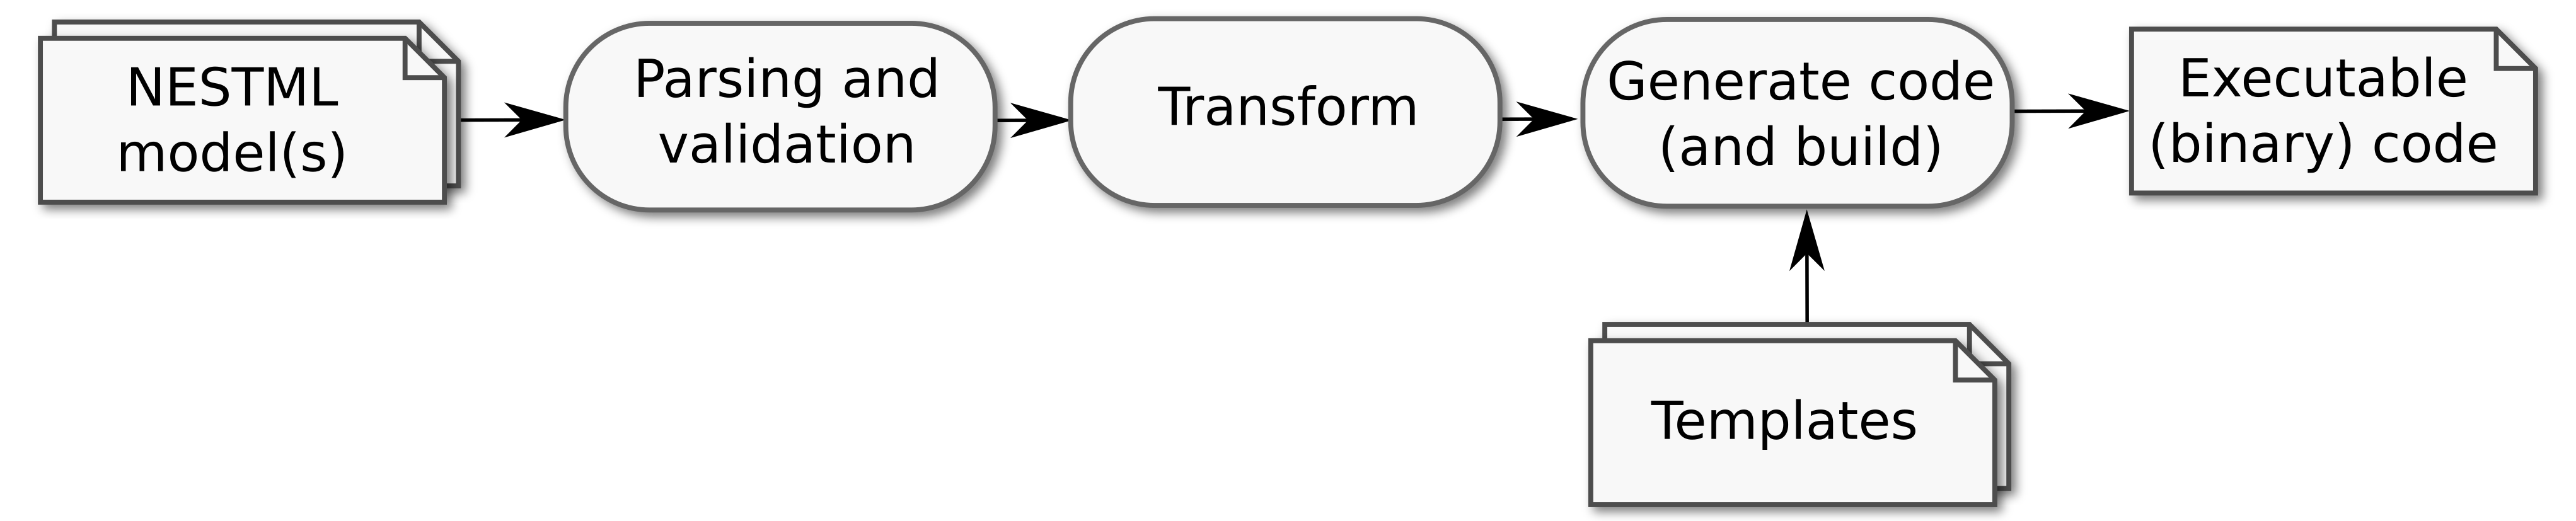
\includegraphics[width=0.8\textwidth]{src/pic/internal_workflow.png}
\caption{\texttt{PyNESTML}: the code generator pipeline}
\source{\url{https://nestml.readthedocs.io/en/latest}}
\label{fig:pynestml_workflow}
\end{figure}



Is the model compiled, built and ready for use, the next step in the simulation is to make use of the model by introducing it to the \emph{NestKernel} and this happens by the call to \texttt{nest.Install()}. Therefore, in the subsequent section, we examine the execution path taken by registering new models in \emph{NEST}.

\section{NestKernel The Simulation Backend}


This section serves as a basic introduction to the most important functionalities that will be affected by the new implementation in \autoref{chap:vec}. Registering new custom models and creating new nodes are the first steps in each simulation script, and usually the user should not worry about how nodes are created. Once the model is registered, the \emph{NestKernel} creates a \emph{factory} object responsible for instantiating nodes from the model and managing any modification made to the model by the user during the simulation. To further understand the \emph{factory} concept in registering and creating nodes, we have to take a deeper look at the source code and inspect the important steps required for making the correct execution of the simulation. In the subsequent section, firstly we review the logic behind registering nodes and secondly, how to create node instances from these models.

From the start, we have mentioned that \emph{PyNEST} is the python interface for executing the \emph{NestKernel} functions. That is actually not totally true. Each function call in \emph{PyNest} is directly forwarded to the \emph{SLI} engine \cite{gewaltig2007nest}. \text{SLI} is a stack-based language derived from PostScript \cite{adobe1990postscript}, and it is outside the scope of the thesis.

Figure \ref{fig:layer} below depicts the three layers that are responsible for running the simulation, from the python interface to the \texttt{C++} layer. \emph{PyNEST} takes the arguments from the simulation scripts and processes the arguments to make them ready for the \emph{SLI} interface functions. \texttt{SLI} then starts objects conversion and calls the exposed functions in the \emph{NestKernel}.

\begin{figure}[h!]
\centering
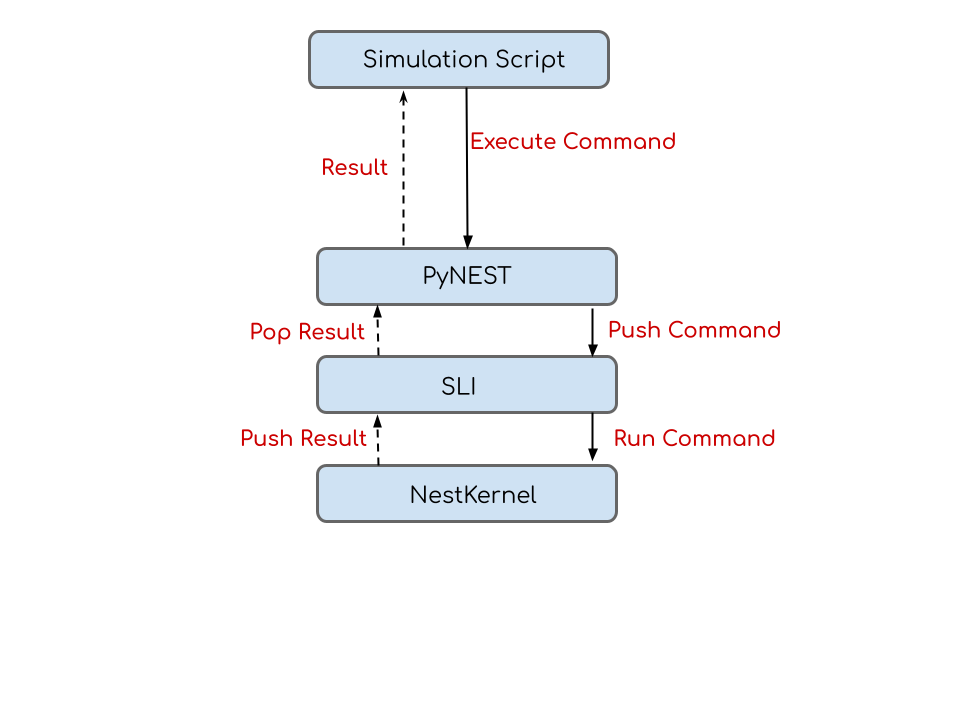
\includegraphics[width=0.8\textwidth]{src/pic/layers.png}
\caption{\texttt{Nest} layers}
\label{fig:layer}
\end{figure}

\subsection{Registering New Models}

For abstraction, we use \texttt{N} as the custom model class type that will be registered and show the workflow in the message sequence diagram depicted in the   \autoref{fig:nestknerl_register}.  Every custom model generated by \emph{PyNESTML} is shipped with two main components (see \autoref{fig:sli_install}). The first component is the implementation of the model in \texttt{C++} and the second component is the derived class from the \texttt{SLIModule}, and it is responsible for registering the model in the \emph{Nestkernel}. By calling the \texttt{nest.Install} function
with the model library name as parameter, \emph{SLI} searches for the library in the provided paths and dynamically loads it. Upon loading, \emph{SLI} calls the \texttt{init()} functions in the derived \texttt{SLIModule} class. The \texttt{SLIModule} instance calls the \texttt{register\_node\_model}  in the \texttt{ModelManager} class. The function required mainly two items. The first is the Class  type name of the model as in the \emph{template} name and secondly, the name of the model that will be available to the user to use. 

the \texttt{register\_node\_model} function checks if there exists another model under the same name and only proceed to registering the model if its name is unique. Afterwards, a new instance of the \texttt{GenericModel<T>} class is created with our model \texttt{N} as the substituted type (i.e., \texttt{T = N}). In fact, the \texttt{GenericModel} class works as a factory responsible for creating the instances of \texttt{N}, which means that  the user can not explicitly call the constructor of \texttt{N} and each creation of \texttt{N} is done by the \texttt{GenericModel}. Finally, the \texttt{ModelManager} takes control again, sets the model parameters (i.e., \texttt{ID}) and lastly creates a \texttt{proxy} objects of the model in each \emph{thread}. The \texttt{proxy} nodes are only required for nodes residing in remote processes, and they are meant for boosting the performance during connections setup and simulation. the \texttt{register\_node\_model} returns then the new \texttt{ID} of the model to \texttt{SLIModule} which itself returns the same \texttt{ID} to the initiator of the \texttt{install} command in \emph{SLI}.
 
 
 \begin{figure}[ht!]
\centering
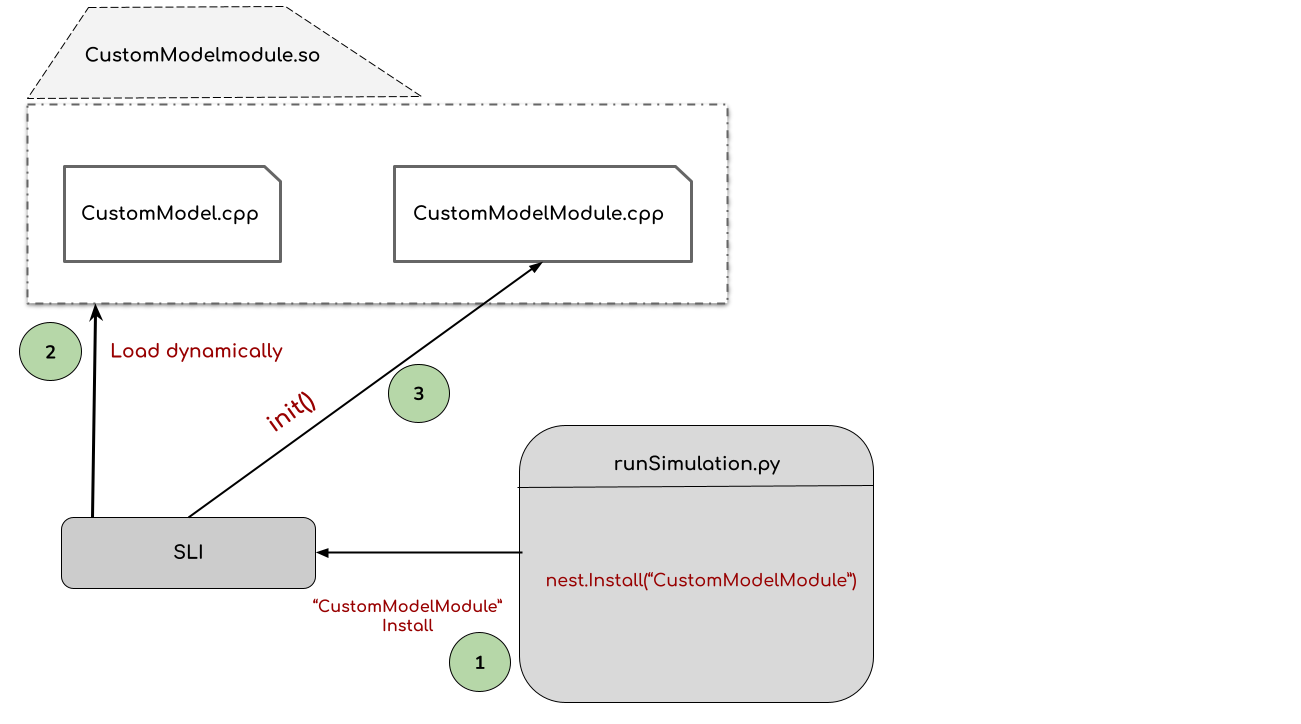
\includegraphics[width=1.2\textwidth,height=1.2\textheight,keepaspectratio]{src/pic/install_command.png}
\caption{\texttt{SLI} installing external module }
\label{fig:sli_install}
\end{figure}

\vspace{0.5cm}
\begin{figure}[ht!]
\centering
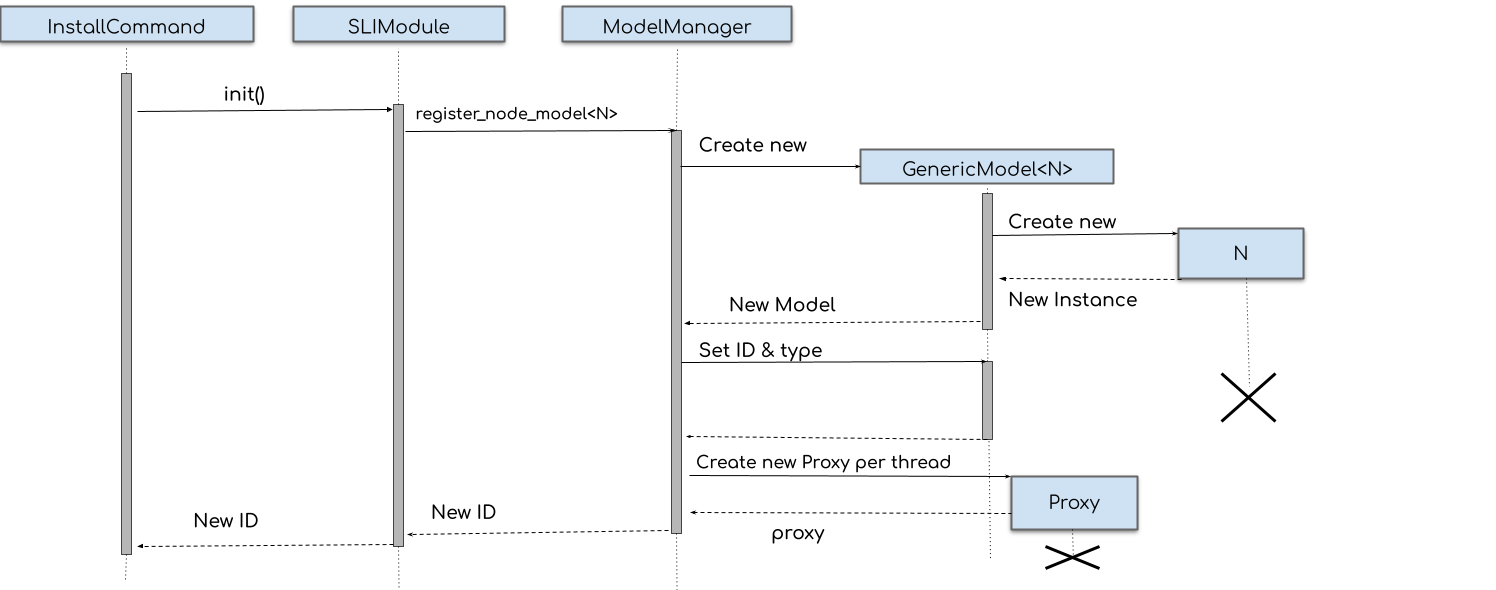
\includegraphics[width=1.2\textwidth,height=1.3\textheight,keepaspectratio]{src/pic/register.png}
\caption{\texttt{NestKernel} registering new models }
\label{fig:nestknerl_register}
\end{figure}

\subsection{Creating New Nodes}

In this subsection, we focus on three components in the \emph{NestKernel}. The \texttt{NodeManager} which is responsible for creating nodes, handling the distribution of nodes over the available \emph{threads}.
It is important to keep in mind that each node is exactly assigned to one thread and each thread can only modify its nodes, non-local nodes are represented by \emph{proxies}. Also, each thread knows the total number of the created nodes. The second component
is the \texttt{GenericModel}, and as we have mentioned in the previous subsection that it plays the role of a \emph{factory} responsible for creating the real instances of the registered model. Finally, the registered model \texttt{N} which provides an implementation for \emph{cloning} that is required of creating new nodes.
Upon requesting the creation of $n$ nodes, the \texttt{NodeMananger} calls the \texttt{GenericModel} to create an instance of the registered model, which just creates a new empty copy of the model and returns it to the \texttt{NodeManager}. \autoref{fig:nestknerl_creation} depicts the steps involved in creating a new node.


\begin{figure}[ht!]
\centering
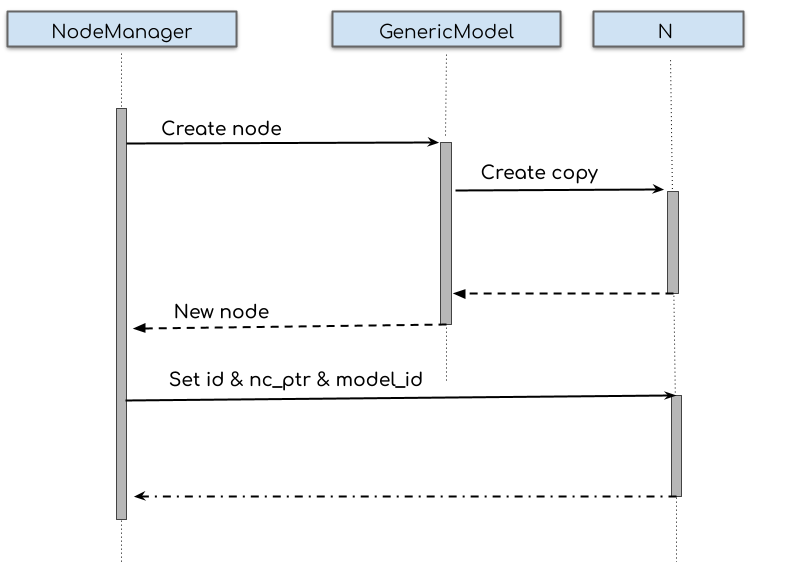
\includegraphics[width=1\textwidth,height=1\textheight,keepaspectratio]{src/pic/nodes_creation.png}
\caption{\texttt{NestKernel}: registering new models }
\label{fig:nestknerl_creation}
\end{figure}


\section{PyNEST The Simulation Frontend}

\emph{PyNEST} and the \emph{NestKernel} are completely separated and independent modules. The only way for both of them to communicate is through the \texttt{SLI} interface. As shown in \autoref{fig:pynest} from \cite{epp}, \emph{PyNEST} is split into two layers. The \emph{low-level API} is responsible for ensuring the smooth communication between \emph{Python} and \emph{SLI} by providing the necessary functionalities for converting data from \emph{SLI} to \emph{Python} and vice versa. The \emph{low-level API} is based on the \emph{Python C API}. It uses mainly three functions to communicate with \emph{SLI}. The \texttt{sli\_push()} function for pushing the function's arguments of the \emph{SLI} command onto the stack, \texttt{sli\_pop} for retrieving the returned value of the command from the stack and finally the \texttt{sli\_run} for executing the command.  the \texttt{sli\_push} and \texttt{sli\_pop} are also responsible for converting the data (arguments and results) between both interfaces.



 The \emph{high-level API} provides the necessary functions for creating the network and running the simulation. Using the three provided functions in the \emph{low-level API} is not convenient and might not be very intuitive. Therefore, the \emph{high-level API} solves this problem by wrapping the \texttt{SLI} functions. It covers all the functionalities in \emph{SLI} by using the functions from the \emph{low-level API}, making all \emph{SLI} commands available.
 
 Each simulation script is based on the \emph{high-level API} functions. The \texttt{Create} function is responsible for creating new instances of the registered models. It takes four parameters, the model name, the number of instances, the new model parameters values and lastly a spatial distribution of the nodes. Only the model name is a required parameter, and the others are optional. Omitting the number of instances, the \texttt{Create} function returns one single instance. Discarding the model parameters values, the created node will have the default model values and finally, the nodes will not have any spatial distribution if the \texttt{spatial} parameter is omitted. The returned value of the function is a \texttt{NodeCollection} object. The \texttt{NodeCollection} class is a compact representation of the nodes in the \texttt{high-level API} interface. Apart from the \texttt{Create} function, all functions in \emph{PyNEST} expect a \texttt{NodeCollection} object in order to query or modify the created nodes. The \texttt{NodeCollection} stores only the \texttt{ids} of the nodes it contains, and thus less conversion overhead between \emph{SLI} and \emph{PyNEST}. 



An important feature of the \texttt{NodeCollection} class, that it only stores a contiguous set of nodes. Thus, creating many nodes only requires storing the position of the first and the last position of the nodes in the list. Thus, the \texttt{NodeCollection} always holds a list of contiguous blocks. Since the class is also \emph{iterable}, it supports indexing, splitting and concatenating.  


The \texttt{NodeCollection} allows also retrieve different values from the created nodes by calling the \texttt{get} functions. Depending on the number of provided keys, the \texttt{get} function returns either a \emph{list} or \emph{dictionary} containing the values of the given keys. We can also change the values by calling the \texttt{set} function. Setting is a bit complicated, as the given value might have different interpretation in the \emph{NestKernel}. Depending on the number of the nodes in the \texttt{NodeCollection} and the type of value (\emph{single} or \emph{list}), the setting might affect single nodes or all of them.

Another important feature is copying models. \emph{PyNEST} and \texttt{Nestkernel} allow users to copy existing models and assign them a new name and different \emph{default-initial} values. The function responsible for copying the models is called \texttt{CopyModel}.

Creating a network is made by calling the \texttt{Connect} function that takes two \texttt{NodeCollection} objects as the \emph{pre-synaptic (source)} and \emph{post-synaptic (target)} elements with extra parameters specifying the type of the connection and a set of rules defining the connection rules (i.e., controlling degree).

finally, we have the \texttt{Simulate} function  with the time $t$ as parameter, which simulates the created network for $t$ milliseconds.

Of course the \emph{PyNEST} module has other important functions to provide, like inspecting the topology of the created network, changing the number of working threads and configuring the \emph{kernel} attributes, but we are mainly interested in the above-mentioned functions that will be used in designing and implementing the architecture for the \emph{JIT} module in the following chapter.
 
 
\vspace{0.5cm}
\begin{figure}[ht!]
\centering
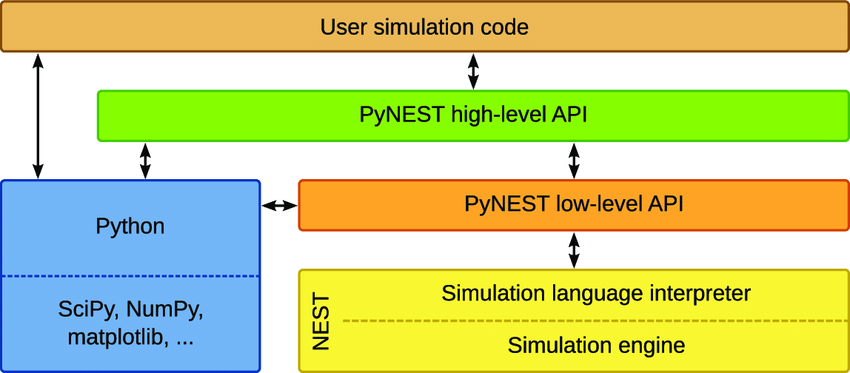
\includegraphics[width=1\textwidth,height=1\textheight,keepaspectratio]{src/pic/The-architecture-of-PyNEST-The-lowest-level-is-the-simulation-engine-It-is-used-by.png}
\caption{The architecture of \emph{PyNest}}
\label{fig:pynest}
\end{figure}






\chapter{Design of the JIT mechanism}
\label{chap:jit}

The focus of this chapter is on concepts for the integration of \emph{just-in-time} (\emph{JIT}) compilation for NESTML models into the PyNEST workflow in a way that is fully backwards compatible and does not require any changes to the PyNEST API. As in any software development process, we start by listing the requirements that the JIT mechanism must fulfil. We then discuss different appects of our design decisions and finally show what possible implications the new software layer will actually have on simulation scripts.

\section{Functional requirements}

In order to have a concise understanding of the JIT mechanism and to really evaluate the correctness of the chosen design, we need a list of requirements that should facilitate the communication between the JIT mechanism and PyNEST and cover the different scenarios that may occur during the simulation.

First and foremost, the JIT mechanism should interact with the PyNEST module and the simulation script. This interaction puts certain restrictions on the functionality of the JIT compilation and affects the structure of simulation scripts and how PyNEST interacts with models. In the following sections, we thus list the most important requirements and explain them in detail. We start with requirements coming from the simulation script and continue with those from the PyNEST module.

\subsection*{Simulation script requirements}

\begin{labeling}{alligator}
   \item[/F1/] The user script should not explicitly import the \emph{PyNESTML} module.
   \item[/F2/] Enabling and disabling the JIT mechanism must be possible in a straightforward way.
   \item[/F3/] Having JIT compilation enabled, the simulation script should not differ a lot from the original script.
   \item[/F4/]\label{req:F4} The user should not explicitly specify the name of the neuron/synapse pairs when connecting the network elements.
   \item[/F5/] A model instance should be available after the call to \texttt{Create()}.
\end{labeling}

These five requirements consitute the basic specifications for designing the JIT mechanism. The first requirement states that the user should not explicitly import the \emph{PyNESTML} module in the script, and thus the JIT mechanism itself will decide if the code generator is required or not, or at which point in time it will import it. The second requirement requires that enabling or disabling the JIT mechanism must not be a complex process. The best way to fulfill this is to only have a single a call in Python without any further user interaction. The third requirement ensures that there is no huge deviation between a script that has the JIT mechanism enabled and one that has it disabled. The fourth requirement addresses the problem that when co-generating a neuron together with a synapse model, the names of both will be changed and the user has to manually use the new names when establishing connections that involve the co-generated models. Retrieving information about the model instances or setting their attributes after creation is very common in most of the simulation scripts, and must be granted to fulfill the sixth requirement, which states that the model should be available right after calling the \texttt{Create()} function.

\subsection*{PyNEST module requirements}

\begin{labeling}{alligator}
   \item[/F7/] Running the simulation with or without the JIT mechanism should not affect the network behavior.
   \item[/F8/] The JIT mechanism should not affect the workflow of PyNEST.
   \item[/F9/] Function signatures of the PyNEST high-level API should not be changed when using the JIT mechanism.
\end{labeling}

When creating instances of the model, the user can parametrize it using values drawn from a specified random distribution. When running the simulation script with the JIT mechanism enabled, the result must be correct and \emph{reproducible}. The seventh requirement thus ensures the correctness of the JIT module. The eighth requirement emphasizes that PyNEST should be completely independent and unaware of the existence of the JIT module, while the last requirement is postulates that the signatures of PyNEST API functions should not be changed in order to ease the implementation of the JIT mechanism.

Based on these requirements coming from the user level simulation script and the PyNEST module, we have designed two complementary approaches that would satisfy all requirements. The benefits and drawbacks of the two designs will be discussed in the following section.

\section{Approach 1: Static code analysis}

The first design idea was to create a \emph{static code analysis} tool that would examine the simulation script before actually running it. The tool would analyze the script against a set of defined rules and decide if the code requires a rearrangement of function calls in PyNEST. In addition, it would extract the parameters of the \texttt{Create()} and \texttt{Connect()} function calls and predict the expected amount of memory needed, so that the required storage could be allocated before actually creating the nodes.

\begin{figure}[ht!]
    \centering

\tikzset{every picture/.style={line width=0.75pt}} %set default line width to 0.75pt
\scalebox{0.5}{
  
\begin{tikzpicture}[x=0.75pt,y=0.75pt,yscale=-1,xscale=1]
%uncomment if require: \path (0,799); %set diagram left start at 0, and has height of 799

%Shape: Circle [id:dp27651862623914725]
\draw  [color={rgb, 255:red, 65; green, 117; blue, 5 }  ,draw opacity=1 ][line width=2.25]  (26,78.4) .. controls (26,62.16) and (39.16,49) .. (55.4,49) .. controls (71.64,49) and (84.8,62.16) .. (84.8,78.4) .. controls (84.8,94.64) and (71.64,107.8) .. (55.4,107.8) .. controls (39.16,107.8) and (26,94.64) .. (26,78.4) -- cycle ;
%Rounded Rect [id:dp7282659276986263]
\draw  [color={rgb, 255:red, 65; green, 117; blue, 5 }  ,draw opacity=1 ][line width=2.25]  (129,64) .. controls (129,59.58) and (132.58,56) .. (137,56) -- (252.3,56) .. controls (256.72,56) and (260.3,59.58) .. (260.3,64) -- (260.3,88) .. controls (260.3,92.42) and (256.72,96) .. (252.3,96) -- (137,96) .. controls (132.58,96) and (129,92.42) .. (129,88) -- cycle ;
%Rounded Rect [id:dp47624918039252084]
\draw  [color={rgb, 255:red, 65; green, 117; blue, 5 }  ,draw opacity=1 ][line width=2.25]  (324,62) .. controls (324,57.58) and (327.58,54) .. (332,54) -- (534.8,54) .. controls (539.22,54) and (542.8,57.58) .. (542.8,62) -- (542.8,86) .. controls (542.8,90.42) and (539.22,94) .. (534.8,94) -- (332,94) .. controls (327.58,94) and (324,90.42) .. (324,86) -- cycle ;
%Shape: Diamond [id:dp35876690900505914]
\draw  [color={rgb, 255:red, 65; green, 117; blue, 5 }  ,draw opacity=1 ][line width=2.25]  (430.8,167) -- (503.8,241) -- (430.8,315) -- (357.8,241) -- cycle ;
%Rounded Rect [id:dp527637097767216]
\draw  [color={rgb, 255:red, 65; green, 117; blue, 5 }  ,draw opacity=1 ][line width=2.25]  (332,370) .. controls (332,365.58) and (335.58,362) .. (340,362) -- (522.8,362) .. controls (527.22,362) and (530.8,365.58) .. (530.8,370) -- (530.8,394) .. controls (530.8,398.42) and (527.22,402) .. (522.8,402) -- (340,402) .. controls (335.58,402) and (332,398.42) .. (332,394) -- cycle ;
%Rounded Rect [id:dp3401618625400282]
\draw  [color={rgb, 255:red, 65; green, 117; blue, 5 }  ,draw opacity=1 ][line width=2.25]  (352,449) .. controls (352,444.58) and (355.58,441) .. (360,441) -- (502.8,441) .. controls (507.22,441) and (510.8,444.58) .. (510.8,449) -- (510.8,473) .. controls (510.8,477.42) and (507.22,481) .. (502.8,481) -- (360,481) .. controls (355.58,481) and (352,477.42) .. (352,473) -- cycle ;
%Rounded Rect [id:dp3943666133910868]
\draw  [color={rgb, 255:red, 65; green, 117; blue, 5 }  ,draw opacity=1 ][line width=2.25]  (44.8,449) .. controls (44.8,444.58) and (48.38,441) .. (52.8,441) -- (274.8,441) .. controls (279.22,441) and (282.8,444.58) .. (282.8,449) -- (282.8,473) .. controls (282.8,477.42) and (279.22,481) .. (274.8,481) -- (52.8,481) .. controls (48.38,481) and (44.8,477.42) .. (44.8,473) -- cycle ;
%Rounded Rect [id:dp7256122135221656]
\draw  [color={rgb, 255:red, 65; green, 117; blue, 5 }  ,draw opacity=1 ][line width=2.25]  (111,531) .. controls (111,526.58) and (114.58,523) .. (119,523) -- (211.8,523) .. controls (216.22,523) and (219.8,526.58) .. (219.8,531) -- (219.8,555) .. controls (219.8,559.42) and (216.22,563) .. (211.8,563) -- (119,563) .. controls (114.58,563) and (111,559.42) .. (111,555) -- cycle ;
%Rounded Rect [id:dp5937426008692417]
\draw  [color={rgb, 255:red, 65; green, 117; blue, 5 }  ,draw opacity=1 ][line width=2.25]  (55,629) .. controls (55,624.58) and (58.58,621) .. (63,621) -- (267.8,621) .. controls (272.22,621) and (275.8,624.58) .. (275.8,629) -- (275.8,653) .. controls (275.8,657.42) and (272.22,661) .. (267.8,661) -- (63,661) .. controls (58.58,661) and (55,657.42) .. (55,653) -- cycle ;
%Shape: Circle [id:dp6422531264539151]
\draw  [color={rgb, 255:red, 65; green, 117; blue, 5 }  ,draw opacity=1 ][line width=2.25]  (357,638.4) .. controls (357,622.16) and (370.16,609) .. (386.4,609) .. controls (402.64,609) and (415.8,622.16) .. (415.8,638.4) .. controls (415.8,654.64) and (402.64,667.8) .. (386.4,667.8) .. controls (370.16,667.8) and (357,654.64) .. (357,638.4) -- cycle ;
%Straight Lines [id:da45299673120981465]
\draw [line width=1.5]    (84.8,78.4) -- (124.8,78.59) ;
\draw [shift={(127.8,78.6)}, rotate = 180.27] [color={rgb, 255:red, 0; green, 0; blue, 0 }  ][line width=1.5]    (14.21,-4.28) .. controls (9.04,-1.82) and (4.3,-0.39) .. (0,0) .. controls (4.3,0.39) and (9.04,1.82) .. (14.21,4.28)   ;
%Straight Lines [id:da7350379896053278]
\draw [line width=1.5]    (259.8,74) -- (321.8,73.81) ;
\draw [shift={(324.8,73.8)}, rotate = 179.82] [color={rgb, 255:red, 0; green, 0; blue, 0 }  ][line width=1.5]    (14.21,-4.28) .. controls (9.04,-1.82) and (4.3,-0.39) .. (0,0) .. controls (4.3,0.39) and (9.04,1.82) .. (14.21,4.28)   ;
%Straight Lines [id:da48742271792213954]
\draw [line width=1.5]    (429.8,92.8) -- (430.76,164) ;
\draw [shift={(430.8,167)}, rotate = 269.23] [color={rgb, 255:red, 0; green, 0; blue, 0 }  ][line width=1.5]    (14.21,-4.28) .. controls (9.04,-1.82) and (4.3,-0.39) .. (0,0) .. controls (4.3,0.39) and (9.04,1.82) .. (14.21,4.28)   ;
%Straight Lines [id:da030763451651900642]
\draw [line width=1.5]    (431.4,321) -- (431.77,356) ;
\draw [shift={(431.8,359)}, rotate = 269.4] [color={rgb, 255:red, 0; green, 0; blue, 0 }  ][line width=1.5]    (14.21,-4.28) .. controls (9.04,-1.82) and (4.3,-0.39) .. (0,0) .. controls (4.3,0.39) and (9.04,1.82) .. (14.21,4.28)   ;
%Curve Lines [id:da746841578624819]
\draw [line width=1.5]    (503.8,241) .. controls (543.4,211.3) and (569.28,408.79) .. (511.57,450.58) ;
\draw [shift={(509.8,451.8)}, rotate = 326.98] [color={rgb, 255:red, 0; green, 0; blue, 0 }  ][line width=1.5]    (14.21,-4.28) .. controls (9.04,-1.82) and (4.3,-0.39) .. (0,0) .. controls (4.3,0.39) and (9.04,1.82) .. (14.21,4.28)   ;
%Straight Lines [id:da20240124908584112]
\draw [line width=1.5]    (430.8,404) -- (430.8,437) ;
\draw [shift={(430.8,440)}, rotate = 270] [color={rgb, 255:red, 0; green, 0; blue, 0 }  ][line width=1.5]    (14.21,-4.28) .. controls (9.04,-1.82) and (4.3,-0.39) .. (0,0) .. controls (4.3,0.39) and (9.04,1.82) .. (14.21,4.28)   ;
%Straight Lines [id:da5681696199392479]
\draw [line width=1.5]    (348.8,462) -- (290.8,461.81) ;
\draw [shift={(287.8,461.8)}, rotate = 0.19] [color={rgb, 255:red, 0; green, 0; blue, 0 }  ][line width=1.5]    (14.21,-4.28) .. controls (9.04,-1.82) and (4.3,-0.39) .. (0,0) .. controls (4.3,0.39) and (9.04,1.82) .. (14.21,4.28)   ;
%Straight Lines [id:da5097999418987831]
\draw [line width=1.5]    (160.8,485) -- (160.8,519) ;
\draw [shift={(160.8,522)}, rotate = 270] [color={rgb, 255:red, 0; green, 0; blue, 0 }  ][line width=1.5]    (14.21,-4.28) .. controls (9.04,-1.82) and (4.3,-0.39) .. (0,0) .. controls (4.3,0.39) and (9.04,1.82) .. (14.21,4.28)   ;
%Straight Lines [id:da12364335757200351]
\draw [line width=1.5]    (161.8,569) -- (161.8,612.8) ;
\draw [shift={(161.8,615.8)}, rotate = 270] [color={rgb, 255:red, 0; green, 0; blue, 0 }  ][line width=1.5]    (14.21,-4.28) .. controls (9.04,-1.82) and (4.3,-0.39) .. (0,0) .. controls (4.3,0.39) and (9.04,1.82) .. (14.21,4.28)   ;
%Straight Lines [id:da5822936780343748]
\draw [line width=1.5]    (277.8,639.8) -- (350.8,639.8) ;
\draw [shift={(353.8,639.8)}, rotate = 180] [color={rgb, 255:red, 0; green, 0; blue, 0 }  ][line width=1.5]    (14.21,-4.28) .. controls (9.04,-1.82) and (4.3,-0.39) .. (0,0) .. controls (4.3,0.39) and (9.04,1.82) .. (14.21,4.28)   ;

% Text Node
\draw (32,70.9) node [anchor=north west][inner sep=0.75pt]   [align=left] {{\fontfamily{pcr}\selectfont {\large \textcolor[rgb]{0.25,0.46,0.02}{\textbf{Start}}}}};
% Text Node
\draw (144,69) node [anchor=north west][inner sep=0.75pt]   [align=left] {{\fontfamily{pcr}\selectfont \textcolor[rgb]{0.25,0.46,0.02}{\textbf{Create Nodes}}}};
% Text Node
\draw (350,66) node [anchor=north west][inner sep=0.75pt]   [align=left] {{\fontfamily{pcr}\selectfont \textcolor[rgb]{0.25,0.46,0.02}{\textbf{Set Node Attributes}}}};
% Text Node
\draw (390,220) node [anchor=north west][inner sep=0.75pt]   [align=left] {{\fontfamily{pcr}\selectfont \textcolor[rgb]{0.25,0.46,0.02}{\textbf{Random}}}\\{\fontfamily{pcr}\selectfont \textcolor[rgb]{0.25,0.46,0.02}{\textbf{Attributes?}}}};
% Text Node
\draw (346,374) node [anchor=north west][inner sep=0.75pt]   [align=left] {{\fontfamily{pcr}\selectfont \textcolor[rgb]{0.25,0.46,0.02}{\textbf{Pre-processing Nodes}}}};
% Text Node
\draw (370,453) node [anchor=north west][inner sep=0.75pt]   [align=left] {{\fontfamily{pcr}\selectfont \textbf{\textcolor[rgb]{0.25,0.46,0.02}{Create Network}}}};
% Text Node
\draw (65,453) node [anchor=north west][inner sep=0.75pt]   [align=left] {{\fontfamily{pcr}\selectfont \textcolor[rgb]{0.25,0.46,0.02}{\textbf{Pre-processing Network}}}};
% Text Node
\draw (130,535) node [anchor=north west][inner sep=0.75pt]   [align=left] {{\fontfamily{pcr}\selectfont \textbf{\textcolor[rgb]{0.25,0.46,0.02}{Simulate}}}};
% Text Node
\draw (65,633) node [anchor=north west][inner sep=0.75pt]   [align=left] {{\fontfamily{pcr}\selectfont \textcolor[rgb]{0.25,0.46,0.02}{\textbf{Post-processing Network}}}};
% Text Node
\draw (372,630) node [anchor=north west][inner sep=0.75pt]   [align=left] {{\fontfamily{pcr}\selectfont \textbf{\textcolor[rgb]{0.25,0.46,0.02}{End}}}};
% Text Node
\draw (395,324) node [anchor=north west][inner sep=0.75pt]   [align=left] {{\fontfamily{pcr}\selectfont \textbf{\textcolor[rgb]{0.55,0.34,0.16}{{\large Yes}}}}};
% Text Node
\draw (545,232) node [anchor=north west][inner sep=0.75pt]   [align=left] {{\fontfamily{pcr}\selectfont {\large \textbf{\textcolor[rgb]{0.55,0.34,0.16}{No}}}}};

\end{tikzpicture}
}

    \caption{The execution flow of any possible simulation: All simulations start by creating an arbitrary number of nodes as instances of the registered models. Model attributes can be either assigned deterministic or random values. If random values are used, the user can inspect the drawn values and check the current state of the nodes before building the network. Similarly to the nodes, creating the network by connecting the nodes can be either be a fully deterministic or a random operation (in both the connection parameters and the connectivity itself). The user can inspect the topology of the network before running the simulation. Both, the network and the nodes might have different states after running the simulation, and those states might be inspected after the simulation to draw conclusions about the behavior of the network and its nodes.}
    \label{fig:simulation_steps}
\end{figure}

%\begin{figure}[ht!]
%\centering
%\includegraphics[width=1.1\textwidth,height=1.2\textheight,keepaspectratio]{src/pic/s%imulation_steps.png}
%\caption{The architecture of \texttt{PyNest} }
%\label{fig:simulation_steps}
%\end{figure}


Unfortunately, this two-pass approach suffers from a severe problem: Simulation scripts can be split into different phases, as depicted in \autoref{fig:simulation_steps}. Usually they start by creating instances of arbitrary models (the \emph{nodes}) and the user may then modify the parameters of these nodes. In case of parameters drawn from a random distribution, the user may want to inspect the chosen values before connecting the nodes to create the network. Similarly, the parameters of the edges of the network (i.e., the \emph{synapses}) may be assigned randomized values that the user might want to inspect prior to the simulation. Due to the static nature of the proposed tool, it cannot take into account all possible ways a user may modify neuronal or synaptic properties after their creation, and thus the tool would not be very flexible.

Rearranging the script to allow for more user flexibility would violate the requirement that the simulation script must not be changed and results must be \emph{reproducible} (\emph{F7}). It may simply not always be possible to control the order of the creation of nodes when function calls get rearranged, which might introduce slight deviations in the script and therefore in the simulation results with the code analysis in place compared to the original simulation script without.

The tool also violates \emph{F4}, as we cannot tell if the \emph{synapse} type involved in creating the connection is a \emph{built-in} synapse or a custom defined synapse just by performing a purely static analysis. This would result in a situation, where the user still has to explicitly provide the name of the \emph{synapse} model coming from the code generator.

To prevent the violation of the requirements mentioned above, the logic of the simulation script could be split into two parts: The first part for the functionalities that do not require the analysis tool, the second for those that do. However, even if we would find a solution to this partition problem, it is obvious that we are again rearranging the code and end up violating the requirements \emph{F8} (reproducibility) and \emph{F3} (deviation from original code).

As the static analysis violates some crucial requirements for preserving the correctness of simulations, we have come up with an alternative approach that should solve the problems of the static analysis tool.


\section{Approach 2: PyNEST Wrapper}

As shown in \autoref{fig:simulation_steps} all simulation scripts other than those simulating an empty network or a network with only a single node contain at least two essential functions, namely \texttt{Create()} and \texttt{Connect()}. The first takes four parameters: the model name, the number of instances to be created, the instance parameters and a spatial arrangement for the instances. In this section, we are only interested in the first parameter, the model name. After installing a new external model, the NestKernel stores it in an array of models. When creating a new instance of the model, the NestKernel searches for the model by its name and once it is found, it creates the required number of instances. A precondition for the \texttt{Create()} function to work is thus to have the models installed and registered in the NestKernel.

The second function that is present in all non-trivial simulation scripts is \texttt{Connect()}. Its five parameters are The source nodes, the target nodes, a dictionary specifying the connection pattern to establish between source and target population, a dictionary for specifying the synapse model and its parameters, and finally a Boolean indicating if the function should return a \texttt{SynapseCollection} object to inspect the created connections. When using both external neuron and synapse models in the connection, the user must explicitly co-generate the neuron and synapse models, providing a mapping between neuronal and synaptic variables (called \emph{port map}) to the code generator before installing them.

The idea of the second approach is to create an interface that controls the NESTML workflow behind the scenes of PyNEST function calls. It is clear that the model's name is sufficient to locate the model, either as in the \texttt{.nestml} file or in the dynamic library. Depending on the situation, we can then either install the module directly or first generate the model's code, build it and then install it. With this new setup, the user can then stop importing the PyNESTML module and explicitly calling the \texttt{Install()} function, as both will be handled transparently in the background when calling the \texttt{Create()} function. Again, it is important to understand that we are not modifying the PyNEST module, we are simply implementing an intermediate interface between the simulation script and the real PyNEST functions, and this new interface would provide the same functions to the simulation script.

This approach works as a \emph{wrapper} around all of PyNEST, so we do not need to have a wrapper around each PyNEST function. It suffices to only choose those \emph{high-level API} functions and intercept their calls and decide either to execute them directly, or apply some logic before and after the real function calls or even disable them altogether. Mathematically described, each function $f$ in PyNEST is replaced by one of the following execution paths:

\begin{align*}
f \mapsto&\enspace\emptyset\\
f \mapsto&\enspace f \circ before \\
f \mapsto&\enspace f \\
f \mapsto&\enspace after \circ f \\
f \mapsto&\enspace after \circ f \circ before\\
f \mapsto&\enspace g:\enspace \text{\#replace the call of } f \text{ with } g \in \{before, after\}  \\
\end{align*}

The empty set ($\emptyset$) means that we intercept the function call, but do nothing (the function will be disabled). The functions \texttt{before} and \texttt{after} represent pre-processing and post-processing steps. For example, when creating instances of the model, the \texttt{before} function could search for the model and ensure that the real \texttt{Create()} function will be called without errors. The \texttt{after} function would return the \emph{NodeCollection} object containing the instances of the model. In this scenario, the real \texttt{Create()} would be called inside the \texttt{before} function.

One remaining issue is concerning calls to \texttt{Connect()} and the co-generation of neuron/synapse pairs. Recall that the user must explicitly specify the port connecting both the neuron and the synapse, and this information is handled by the code generator. To tackle this issue and completely remove the use of the code generator in the simulation script, we would have to extend the synapse dictionary object in the \texttt{Connect()} function with a new key referring to the mapping between the neuron and synapse and let the \texttt{before} function processes the dictionary and remove the inserted key before it forwards it to the code generator. Once the co-generation is finished, we can then call the real \emph{Connect()} function in PyNEST.

This approach might sound simple at first glance, but a lot has to happen behind the scene, as new components are introduced that facilitate the interception of PyNEST functions calls. All required components are discussed in detail in the subsequent sections by introducing their roles and how they can be used and how they ensure the fulfillment of all functional requirements as laid out above.



\section{JIT Design: The Big Picture}

In order for the \emph{JIT} to work with respect to the given requirements, we have come with certain necessary components that facilitate the workflow. As depicted in \autoref{fig:jit_module} under the \texttt{models}, we have the essential components responsible for representing and managing the models as python objects before making them available to the \emph{NestKernel}. The \texttt{jit\_model} stores information about the chosen \emph{nestml} model by storing its parameters and states and making it possible for the user to query on those attributes after creating the instances of the model. Secondly, we have the \texttt{model\_query} which is important for searching the model either in the \emph{nestml} files or in the created libraries. Depending on which format, the \texttt{model\_query} returns an instance of the \texttt{model\_handle}, which is responsible for making the model available to the \emph{NestKernel}. The  \texttt{model\_handle} knows if the model is coming from a \emph{nestml} file, and therefore can initiate the code generation process and install the model. On the other hand, if the model is coming from an already existing library, it will just install the model. The \texttt{model\_manager} is responsible for storing all created objects in the \emph{JIT} module, and it is the only way to communicate with the \emph{PyNEST} module. Additionally, the \texttt{model\_manager} manages the mapping of \emph{IDs} between the created models on the python side and the real models coming from the \emph{NestKernel} with the help of the \texttt{model\_indexer}. Finally, under the \texttt{models} directory, we have the \texttt{node\_collection\_proxy} that mimics the behavior of the \texttt{nest.NodeCollection} in \emph{PyNEST} and it provides all functionalities like the \texttt{Setter/Getter} and \emph{Indexing/Slicing}. The need for such a class will be explained later on in this chapter. 


Under the \texttt{utils} directory, we have the needed components responsible for creating a \emph{lightweight} version of the \emph{nestml} models and controlling the code generation steps. The reason behind using a \emph{lightweight} version should also be clear in the following sections.

Furthermore, we have the \texttt{wrapper} directory containing the necessary logic for wrapping the \emph{PyNEST} targeted functions. In the \texttt{Wrapper.py} we have the \texttt{Wrapper} interface that contains the basic code needed for each wrapper to control the targeted functions and under \texttt{Wrappers.py} we have the derived concrete implementation of the \texttt{Wrapper}. Any further custom wrapping functionality should be added there, and it will be automatically registered. Details about how we can create a custom wrapper will be given later.

Finally, we have the \texttt{nest\_manager} which initiates the process of wrapping the \emph{PyNEST} module and calling the implemented wrappers for each target function. The \texttt{\_\_init\_\_} is obviously the starting point of the \emph{JIT} that starts the \texttt{nest\_manager} and overrides the \texttt{import} function in python in order to delegate any further imports from \emph{PyNEST} and add them to the \emph{JIT}.



\begin{figure}[ht!]
\centering
\resizebox{\textwidth}{!}{
    \begin{tikzpicture}[
      level 1/.style={sibling distance=50mm},
      edge from parent/.style={->,draw},
      >=latex]
    
    % root of the the initial tree, level 1
    \node[root] {JIT}
    % The first level, as children of the initial tree
      child {node[level 2] (c1) {interfaces}}
      child {node[level 2] (c2) {models}}
      child {node[level 2] (c3) {utils}}
      child {node[level 2] (c4) {wrapper}}
      child {node[level 2] (c5) {nest\_manager.py}}
      child {node[level 2] (c6) {\_\_init\_\_.py}};
    
    % The second level, relatively positioned nodes
    \begin{scope}[every node/.style={level 3}]
    \node [below of = c1, xshift=25pt] (c11) {jit\_interface.py};
    
    \node [below of = c2, xshift=25pt] (c21) {jit\_model.py};
    \node [below of = c21] (c22) {model\_query.py};
    \node [below of = c22] (c23) {model\_indexer.py};
    \node [below of = c23] (c24) {model\_manager.py};
    \node [below of = c24] (c25) {model\_handle.py};
    \node [below of = c25] (c26) {node\_collection\_proxy.py};
    
    
    \node [below of = c3, xshift=25pt, fill=red!20] (c31) {templates};
    \node [below of = c31] (c32) {report.py};
    \node [below of = c32] (c33) {jit\_model\_parser.py};
    \node [below of = c33] (c34) {nest\_config.py};
    \node [below of = c34] (c35) {symbols.py};
    \node [below of = c35] (c36) {thread\_manager.py};
    \node [below of = c36] (c37) {utils.py};
    
    
    \node [below of = c4, xshift=25pt] (c41) {wrapper.py};
    \node [below of = c41] (c42) {wrappers.py};
    \node [below of = c42] (c43) {module\_wrapper.py};

    
    \end{scope}
    
    % lines from each level 1 node to every one of its "children"
    \foreach \value in {1}
      \draw[->] (c1.177) |- (c1\value.west);
    
    \foreach \value in {1,...,6}
      \draw[->] (c2.177) |- (c2\value.west);
    
    \foreach \value in {1,...,7}
      \draw[->] (c3.177) |- (c3\value.west);
      
      
    \foreach \value in {1,...,3}
      \draw[->] (c4.177) |- (c4\value.west);
    \end{tikzpicture}
    }
    \caption{the \emph{JIT} module}
    \label{fig:jit_module}

\end{figure}


In order to have a complete overview of what is happening in the back scene of running \emph{JIT}, we explain the important steps in their correct order of execution. We start explaining the wrapping mechanism and how to implement our custom wrapper. Secondly, we explain how the creation of instances look like with \emph{JIT} enabled, and we discuss then how the \texttt{nest.Connect} function might be slightly modified and finally the role of the modified \texttt{nest.Simulate}. As the \texttt{NodeCollectionProxy} is part of the creation calls, we will introduce it in the same section of  the \texttt{nest.Create} wrapper.





\section{JIT Wrappers}

In this section, we introduce the \emph{Wrapper} interface responsible for intercepting the function calls in \emph{PyNEST}, and we discuss the derived classes inheriting from this interface allowing to control the workflow of the targeted functions in \emph{PyNEST}.

\subsection{The Wrapper Base Class}

The \emph{Wrapper} interface as depicted in \autoref{fig:wrapper_uml} shows the essential items that make \emph{JIT} able to intercept and modify the calls to the \emph{high level API} in \emph{PyNESt}. Each \emph{Wrapper} instance has two boolean attributes. The first attribute specifies if we are wrapping a function or a method. The second is to ignore the function call and skip its execution. By default, the second attribute is set to \texttt{false}. As we have mentioned in the previous section, each \emph{Wrapper} object has three main functions to control the interception of the \emph{PyNEST} calls. the \texttt{before} function is mainly responsible for preprocessing the input values that are given to the \emph{PyNEST} function. Secondly, we have the \texttt{main}, which takes the modified parameters from the \texttt{before} function and executes the real \emph{PyNEST} wrapped function. Finally, we have the \texttt{after} function that takes the output of the \texttt{main} function and modifies it if necessary. In addition to those core functions, we have two important functions. The \texttt{get\_name} function that returns the name of the function that we want to wrap, and at last we have the \texttt{wraps\_one} that indicates if this \texttt{Wrapper} object is wrapping one or multiple functions. In the case if it is multiple functions, the \texttt{get\_name} function must return a list containing the names of these functions. One function left which brings all pieces together, the \texttt{\_\_wrapper} as it is responsible for calling the \texttt{before}, \texttt{main} and \texttt{after} functions.


\begin{figure}[ht!]
\centering
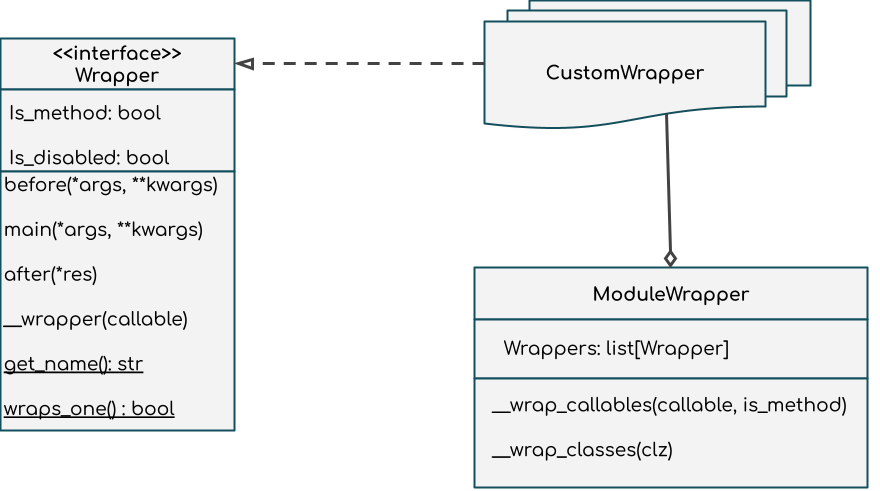
\includegraphics[width=\textwidth,height=\textheight,keepaspectratio]{src/pic/wrapper_uml.png}
\caption{The Wrapper interface}
\label{fig:wrapper_uml}
\end{figure}

The \texttt{ModuleWrapper} is responsible for matching the custom implemented wrappers with the targeted \emph{PyNEST} objects. It iterates overs all functions and classes and replaces them with their corresponding wrappers. finally, we have the \texttt{CustomWrappers} representing the derived classes from the \texttt{Wrapper} interface. Those derived classes can be seen in \autoref{fig:wrapper_derived}.

\subsection{The Wrapper Derived Classes}

The \emph{Wrapper} interface on its own does not do a lot for the \emph{JIT} project, and it requires having a concrete implementation for each function we want to control its workflow. Each derived class from the \emph{Wrapper} interface wraps either a \emph{function} or a \emph{class} in \emph{PyNEST}. As shown in \autoref{fig:wrapper_derived}, we depict the current implemented \emph{wrappers}. Most of these wrappers use a \texttt{helper} class that does all the required logic to make \emph{JIT} work. In the following, we list the implemented wrappers and discuss their usage.

\begin{figure}[ht!]
\centering


\tikzset{every picture/.style={line width=0.75pt}} %set default line width to 0.75pt        

\begin{tikzpicture}[x=0.75pt,y=0.75pt,yscale=-1,xscale=1]
%uncomment if require: \path (0,519); %set diagram left start at 0, and has height of 519

%Rounded Rect [id:dp08332665529733485] 
\draw  [color={rgb, 255:red, 139; green, 87; blue, 42 }  ,draw opacity=1 ][line width=2.25]  (277,217) .. controls (277,212.58) and (280.58,209) .. (285,209) -- (395.8,209) .. controls (400.22,209) and (403.8,212.58) .. (403.8,217) -- (403.8,241) .. controls (403.8,245.42) and (400.22,249) .. (395.8,249) -- (285,249) .. controls (280.58,249) and (277,245.42) .. (277,241) -- cycle ;
%Rounded Rect [id:dp643201073355989] 
\draw  [color={rgb, 255:red, 139; green, 87; blue, 42 }  ,draw opacity=1 ][line width=2.25]  (1.8,427) .. controls (1.8,422.58) and (5.38,419) .. (9.8,419) -- (191.8,419) .. controls (196.22,419) and (199.8,422.58) .. (199.8,427) -- (199.8,451) .. controls (199.8,455.42) and (196.22,459) .. (191.8,459) -- (9.8,459) .. controls (5.38,459) and (1.8,455.42) .. (1.8,451) -- cycle ;
%Rounded Rect [id:dp9738213759503345] 
\draw  [color={rgb, 255:red, 139; green, 87; blue, 42 }  ,draw opacity=1 ][line width=2.25]  (2.8,262) .. controls (2.8,257.58) and (6.38,254) .. (10.8,254) -- (136.8,254) .. controls (141.22,254) and (144.8,257.58) .. (144.8,262) -- (144.8,286) .. controls (144.8,290.42) and (141.22,294) .. (136.8,294) -- (10.8,294) .. controls (6.38,294) and (2.8,290.42) .. (2.8,286) -- cycle ;
%Rounded Rect [id:dp39360724795655755] 
\draw  [color={rgb, 255:red, 139; green, 87; blue, 42 }  ,draw opacity=1 ][line width=2.25]  (503,349) .. controls (503,344.58) and (506.58,341) .. (511,341) -- (645.8,341) .. controls (650.22,341) and (653.8,344.58) .. (653.8,349) -- (653.8,373) .. controls (653.8,377.42) and (650.22,381) .. (645.8,381) -- (511,381) .. controls (506.58,381) and (503,377.42) .. (503,373) -- cycle ;
%Rounded Rect [id:dp2385264912044227] 
\draw  [color={rgb, 255:red, 139; green, 87; blue, 42 }  ,draw opacity=1 ][line width=2.25]  (255.8,480) .. controls (255.8,475.58) and (259.38,472) .. (263.8,472) -- (444.8,472) .. controls (449.22,472) and (452.8,475.58) .. (452.8,480) -- (452.8,504) .. controls (452.8,508.42) and (449.22,512) .. (444.8,512) -- (263.8,512) .. controls (259.38,512) and (255.8,508.42) .. (255.8,504) -- cycle ;
%Rounded Rect [id:dp04455155996593918] 
\draw  [color={rgb, 255:red, 139; green, 87; blue, 42 }  ,draw opacity=1 ][line width=2.25]  (153.8,33) .. controls (153.8,28.58) and (157.38,25) .. (161.8,25) -- (319.8,25) .. controls (324.22,25) and (327.8,28.58) .. (327.8,33) -- (327.8,57) .. controls (327.8,61.42) and (324.22,65) .. (319.8,65) -- (161.8,65) .. controls (157.38,65) and (153.8,61.42) .. (153.8,57) -- cycle ;
%Rounded Rect [id:dp5139694395821088] 
\draw  [color={rgb, 255:red, 139; green, 87; blue, 42 }  ,draw opacity=1 ][line width=2.25]  (5.8,100) .. controls (5.8,95.58) and (9.38,92) .. (13.8,92) -- (137.8,92) .. controls (142.22,92) and (145.8,95.58) .. (145.8,100) -- (145.8,124) .. controls (145.8,128.42) and (142.22,132) .. (137.8,132) -- (13.8,132) .. controls (9.38,132) and (5.8,128.42) .. (5.8,124) -- cycle ;
%Rounded Rect [id:dp796653880823329] 
\draw  [color={rgb, 255:red, 139; green, 87; blue, 42 }  ,draw opacity=1 ][line width=2.25]  (3.8,181) .. controls (3.8,176.58) and (7.38,173) .. (11.8,173) -- (129.8,173) .. controls (134.22,173) and (137.8,176.58) .. (137.8,181) -- (137.8,205) .. controls (137.8,209.42) and (134.22,213) .. (129.8,213) -- (11.8,213) .. controls (7.38,213) and (3.8,209.42) .. (3.8,205) -- cycle ;
%Rounded Rect [id:dp8115528255145159] 
\draw  [color={rgb, 255:red, 139; green, 87; blue, 42 }  ,draw opacity=1 ][line width=2.25]  (1.8,349) .. controls (1.8,344.58) and (5.38,341) .. (9.8,341) -- (159.8,341) .. controls (164.22,341) and (167.8,344.58) .. (167.8,349) -- (167.8,373) .. controls (167.8,377.42) and (164.22,381) .. (159.8,381) -- (9.8,381) .. controls (5.38,381) and (1.8,377.42) .. (1.8,373) -- cycle ;
%Rounded Rect [id:dp6414618614909982] 
\draw  [color={rgb, 255:red, 139; green, 87; blue, 42 }  ,draw opacity=1 ][line width=2.25]  (480.8,268) .. controls (480.8,263.58) and (484.38,260) .. (488.8,260) -- (645.8,260) .. controls (650.22,260) and (653.8,263.58) .. (653.8,268) -- (653.8,292) .. controls (653.8,296.42) and (650.22,300) .. (645.8,300) -- (488.8,300) .. controls (484.38,300) and (480.8,296.42) .. (480.8,292) -- cycle ;
%Rounded Rect [id:dp7381489249035267] 
\draw  [color={rgb, 255:red, 139; green, 87; blue, 42 }  ,draw opacity=1 ][line width=2.25]  (485.8,182) .. controls (485.8,177.58) and (489.38,174) .. (493.8,174) -- (648.8,174) .. controls (653.22,174) and (656.8,177.58) .. (656.8,182) -- (656.8,206) .. controls (656.8,210.42) and (653.22,214) .. (648.8,214) -- (493.8,214) .. controls (489.38,214) and (485.8,210.42) .. (485.8,206) -- cycle ;
%Rounded Rect [id:dp704574691668346] 
\draw  [color={rgb, 255:red, 139; green, 87; blue, 42 }  ,draw opacity=1 ][line width=2.25]  (476.8,102) .. controls (476.8,97.58) and (480.38,94) .. (484.8,94) -- (645.8,94) .. controls (650.22,94) and (653.8,97.58) .. (653.8,102) -- (653.8,126) .. controls (653.8,130.42) and (650.22,134) .. (645.8,134) -- (484.8,134) .. controls (480.38,134) and (476.8,130.42) .. (476.8,126) -- cycle ;
%Rounded Rect [id:dp33221553170106266] 
\draw  [color={rgb, 255:red, 139; green, 87; blue, 42 }  ,draw opacity=1 ][line width=2.25]  (381.8,32) .. controls (381.8,27.58) and (385.38,24) .. (389.8,24) -- (547.8,24) .. controls (552.22,24) and (555.8,27.58) .. (555.8,32) -- (555.8,56) .. controls (555.8,60.42) and (552.22,64) .. (547.8,64) -- (389.8,64) .. controls (385.38,64) and (381.8,60.42) .. (381.8,56) -- cycle ;
%Rounded Rect [id:dp11416390733512127] 
\draw  [color={rgb, 255:red, 139; green, 87; blue, 42 }  ,draw opacity=1 ][line width=2.25]  (499,425) .. controls (499,420.58) and (502.58,417) .. (507,417) -- (641.8,417) .. controls (646.22,417) and (649.8,420.58) .. (649.8,425) -- (649.8,449) .. controls (649.8,453.42) and (646.22,457) .. (641.8,457) -- (507,457) .. controls (502.58,457) and (499,453.42) .. (499,449) -- cycle ;
%Straight Lines [id:da7321475284754999] 
\draw [line width=1.5]  [dash pattern={on 1.69pt off 2.76pt}]  (144.8,113.6) -- (273.85,214.54) ;
\draw [shift={(277,217)}, rotate = 218.03] [fill={rgb, 255:red, 0; green, 0; blue, 0 }  ][line width=0.08]  [draw opacity=0] (11.61,-5.58) -- (0,0) -- (11.61,5.58) -- cycle    ;
%Straight Lines [id:da826027105738447] 
\draw [line width=1.5]  [dash pattern={on 1.69pt off 2.76pt}]  (141.8,191.6) -- (270.92,224.61) ;
\draw [shift={(274.8,225.6)}, rotate = 194.34] [fill={rgb, 255:red, 0; green, 0; blue, 0 }  ][line width=0.08]  [draw opacity=0] (11.61,-5.58) -- (0,0) -- (11.61,5.58) -- cycle    ;
%Straight Lines [id:da9419415019749295] 
\draw [line width=1.5]  [dash pattern={on 1.69pt off 2.76pt}]  (144.8,272.6) -- (269.98,233.78) ;
\draw [shift={(273.8,232.6)}, rotate = 162.77] [fill={rgb, 255:red, 0; green, 0; blue, 0 }  ][line width=0.08]  [draw opacity=0] (11.61,-5.58) -- (0,0) -- (11.61,5.58) -- cycle    ;
%Straight Lines [id:da2009447559522246] 
\draw [line width=1.5]  [dash pattern={on 1.69pt off 2.76pt}]  (169.8,364.6) -- (274.38,244.02) ;
\draw [shift={(277,241)}, rotate = 130.94] [fill={rgb, 255:red, 0; green, 0; blue, 0 }  ][line width=0.08]  [draw opacity=0] (11.61,-5.58) -- (0,0) -- (11.61,5.58) -- cycle    ;
%Curve Lines [id:da7600537285509692] 
\draw [line width=1.5]  [dash pattern={on 1.69pt off 2.76pt}]  (191.8,419) .. controls (249.32,402.03) and (261.22,290.39) .. (298.85,255.16) ;
\draw [shift={(301.8,252.6)}, rotate = 141.34] [fill={rgb, 255:red, 0; green, 0; blue, 0 }  ][line width=0.08]  [draw opacity=0] (11.61,-5.58) -- (0,0) -- (11.61,5.58) -- cycle    ;
%Straight Lines [id:da1297385545876295] 
\draw [line width=1.5]  [dash pattern={on 1.69pt off 2.76pt}]  (345.8,472.6) -- (341.09,255) ;
\draw [shift={(341,251)}, rotate = 88.76] [fill={rgb, 255:red, 0; green, 0; blue, 0 }  ][line width=0.08]  [draw opacity=0] (11.61,-5.58) -- (0,0) -- (11.61,5.58) -- cycle    ;
%Curve Lines [id:da8119155428391331] 
\draw [line width=1.5]  [dash pattern={on 1.69pt off 2.76pt}]  (492.8,433.6) .. controls (470.6,411.4) and (399.99,291.43) .. (381.59,258.8) ;
\draw [shift={(379.8,255.6)}, rotate = 60.95] [fill={rgb, 255:red, 0; green, 0; blue, 0 }  ][line width=0.08]  [draw opacity=0] (11.61,-5.58) -- (0,0) -- (11.61,5.58) -- cycle    ;
%Straight Lines [id:da43888705895379454] 
\draw [line width=1.5]  [dash pattern={on 1.69pt off 2.76pt}]  (500.8,367.6) -- (406.23,244.18) ;
\draw [shift={(403.8,241)}, rotate = 52.54] [fill={rgb, 255:red, 0; green, 0; blue, 0 }  ][line width=0.08]  [draw opacity=0] (11.61,-5.58) -- (0,0) -- (11.61,5.58) -- cycle    ;
%Straight Lines [id:da38095702214592175] 
\draw [line width=1.5]  [dash pattern={on 1.69pt off 2.76pt}]  (479.8,274.6) -- (411.17,230.75) ;
\draw [shift={(407.8,228.6)}, rotate = 32.57] [fill={rgb, 255:red, 0; green, 0; blue, 0 }  ][line width=0.08]  [draw opacity=0] (11.61,-5.58) -- (0,0) -- (11.61,5.58) -- cycle    ;
%Straight Lines [id:da685328333847449] 
\draw [line width=1.5]  [dash pattern={on 1.69pt off 2.76pt}]  (486.8,192.6) -- (407.64,215.87) ;
\draw [shift={(403.8,217)}, rotate = 343.62] [fill={rgb, 255:red, 0; green, 0; blue, 0 }  ][line width=0.08]  [draw opacity=0] (11.61,-5.58) -- (0,0) -- (11.61,5.58) -- cycle    ;
%Straight Lines [id:da09283567688019034] 
\draw [line width=1.5]  [dash pattern={on 1.69pt off 2.76pt}]  (473.8,119.6) -- (398.43,205.99) ;
\draw [shift={(395.8,209)}, rotate = 311.1] [fill={rgb, 255:red, 0; green, 0; blue, 0 }  ][line width=0.08]  [draw opacity=0] (11.61,-5.58) -- (0,0) -- (11.61,5.58) -- cycle    ;
%Curve Lines [id:da7212396930412046] 
\draw [line width=1.5]  [dash pattern={on 1.69pt off 2.76pt}]  (395.8,67.6) .. controls (378.34,64.69) and (399.46,164.34) .. (385.22,203.18) ;
\draw [shift={(383.8,206.6)}, rotate = 295.28] [fill={rgb, 255:red, 0; green, 0; blue, 0 }  ][line width=0.08]  [draw opacity=0] (11.61,-5.58) -- (0,0) -- (11.61,5.58) -- cycle    ;
%Straight Lines [id:da6247278152361431] 
\draw [line width=1.5]  [dash pattern={on 1.69pt off 2.76pt}]  (241.8,68.6) -- (337.46,201.35) ;
\draw [shift={(339.8,204.6)}, rotate = 234.22] [fill={rgb, 255:red, 0; green, 0; blue, 0 }  ][line width=0.08]  [draw opacity=0] (11.61,-5.58) -- (0,0) -- (11.61,5.58) -- cycle    ;

% Text Node
\draw (311,229) node [anchor=north west][inner sep=0.75pt]   [align=left] {{\fontfamily{pcr}\selectfont \textcolor[rgb]{0.55,0.34,0.16}{\textbf{Wrapper}}}};
% Text Node
\draw (8,430) node [anchor=north west][inner sep=0.75pt]   [align=left] {{\fontfamily{pcr}\selectfont \textbf{\textcolor[rgb]{0.55,0.34,0.16}{NodeCollectionWrapper}}}};
% Text Node
\draw (8,265) node [anchor=north west][inner sep=0.75pt]   [align=left] {{\fontfamily{pcr}\selectfont \textbf{\textcolor[rgb]{0.55,0.34,0.16}{DisableNestFunc}}}};
% Text Node
\draw (515,352) node [anchor=north west][inner sep=0.75pt]   [align=left] {\textbf{\textcolor[rgb]{0.55,0.34,0.16}{{\fontfamily{pcr}\selectfont GetStatusWrapper}}}};
% Text Node
\draw (265,482.5) node [anchor=north west][inner sep=0.75pt]   [align=left] {\textbf{\textcolor[rgb]{0.55,0.34,0.16}{\textbf{GetConnectionWrapper}}}};
% Text Node
\draw (175,38) node [anchor=north west][inner sep=0.75pt]   [align=left] {{\fontfamily{pcr}\selectfont \textcolor[rgb]{0.55,0.34,0.16}{\textbf{ConnectWrapper}}}};
% Text Node
\draw (20,103) node [anchor=north west][inner sep=0.75pt]   [align=left] {{\fontfamily{pcr}\selectfont \textbf{\textcolor[rgb]{0.55,0.34,0.16}{CreateWrapper}}}};
% Text Node
\draw (23,184) node [anchor=north west][inner sep=0.75pt]   [align=left] {\textbf{\textcolor[rgb]{0.55,0.34,0.16}{{\fontfamily{pcr}\selectfont ModelWrapper}}}};
% Text Node
\draw (11,352) node [anchor=north west][inner sep=0.75pt]   [align=left] {{\fontfamily{pcr}\selectfont \textbf{\textcolor[rgb]{0.55,0.34,0.16}{SimulationWrapper}}}};
% Text Node
\draw (492.3,273) node [anchor=north west][inner sep=0.75pt]   [align=left] {{\fontfamily{pcr}\selectfont \textbf{\textcolor[rgb]{0.55,0.34,0.16}{RestKernelWrapper}}}};
% Text Node
\draw (491,186) node [anchor=north west][inner sep=0.75pt]   [align=left] {\textbf{\textcolor[rgb]{0.55,0.34,0.16}{{\fontfamily{pcr}\selectfont GetDefaultsWrapper}}}};
% Text Node
\draw (487,106) node [anchor=north west][inner sep=0.75pt]   [align=left] {\textbf{\textcolor[rgb]{0.55,0.34,0.16}{{\fontfamily{pcr}\selectfont SetDefaultsWrapper}}}};
% Text Node
\draw (398,37) node [anchor=north west][inner sep=0.75pt]   [align=left] {{\fontfamily{pcr}\selectfont \textcolor[rgb]{0.55,0.34,0.16}{\textbf{CopyModelWrapper}}}};
% Text Node
\draw (505,430) node [anchor=north west][inner sep=0.75pt]   [align=left] {\textbf{\textcolor[rgb]{0.55,0.34,0.16}{{\fontfamily{pcr}\selectfont SetStatusWrapper}}}};
% Text Node
\draw (285,213) node [anchor=north west][inner sep=0.75pt]   [align=left] {{\fontfamily{pcr}\selectfont \textcolor[rgb]{0.55,0.34,0.16}{≪interface≫}}};


\end{tikzpicture}

\caption{The Wrapper's derived classes}
\label{fig:wrapper_derived}
\end{figure}




\begin{itemize}
   \item CreateWrapper: responsible for searching for the model in the \emph{file system} and in the \emph{NestKernel} built-in models and creating instances from it. \\
   
   \item ConnectWrapper:  responsible for making sure that we are always using the right model while calling the \texttt{nest.Connect} function. It may swap network elements depending on some conditions. \\
   
   \item CopyModelWrapper: shares the same functionality as the \texttt{CreateWrapper} for searching and installing the model in the \emph{NestKernel}. In addition, it creates a copy of the found model.
   
   \item SetStatusWrapper/GetStatusWrapper: set/get the status of the model's instances.\\
   
   
   \item SetDefaultWrapper/GetDefaultWrapper: set/get the default values of the model. Even if the model is not yet registered in the \emph{NestKernel}, the user can create  instances of the copied model.\\
   
   \item GetConnectionWrapper: returns the existing connections between source and target.
   
   \item ResetKernelWrapper: resets both the \emph{JIT} stored information about the models and  calls the \texttt{nest.ResetKerenel} function.\\
   
   \item NodeCollectionWrapper: returns an object containing the real object from the \emph{NestKernel} and the \emph{JIT} instances.\\
   
   \item ModelWrapper: returns all registered models from both the \emph{JIT} and \emph{NestKernel}.\\
   
   \item SimulationWrapper: makes sure that all \emph{JIT} instances are available in the \emph{NestKernel} to start the simulation.\\
   
   \item DisableNestFunc: skips the call of the \emph{PyNEST} function.
\end{itemize}   
   
   In the next step, we explain how to add a new wrapper in \emph{JIT} and explain the workflow behind the most important implemented wrappers. Mainly, the \texttt{CreateWrapper}, \texttt{ConnectWrapper} and \texttt{SimulateWrapper} are of interest, the others should follow the same logic.
   
   
\subsection{Adding a New Wrapper Class}

As shown in \autoref{fig:custom_wrapper}, wrapping a new function or class in \emph{PyNEST} is very simple. We only need to add the new implementation to the \texttt{wrapper.py} python file containing all implemented wrappers. At this point, there are no restrictions to how the \texttt{before-main-after} functions must be implemented. The implemented wrapper has the complete  control on how the target \emph{PyNEST} function should behave with respect to \emph{JIT}.


It is also important to know that the developer is not really required to provide an  implementation to the \texttt{before}, \texttt{main} and \texttt{after} functions. As for the default behavior of the \texttt{before} function will just return the input parameters unchanged, the \texttt{main} function calls the real \emph{PyNEST} function and finally the \texttt{after} function checks if \texttt{main} should return and just returns the same object unchanged, otherwise it does nothing.

Registering an custom \emph{Wrapper} is done automatically upon importing the \emph{JIT} module in the python script. In The \texttt{wrappers.py} file, we have the \texttt{install\_wrappers} function shown in \autoref{fig:wrapper_reg} that is responsible for iterating over all the subclasses implementing the \texttt{Wrapper} interface and inserting them in a dictionary, having as \emph{key} the target function name and as \emph{value} the derived wrapper class. The \texttt{ModuleWrapper} imports then the dictionay and iterates over its keys, comparing them with \emph{PyNEST} functions and classes. Once a match is found, the \texttt{ModuleWrapper} creates an instance of the \texttt{CustomWrapper} and extends the \emph{JIT} module with a new function or class having the same name as the one coming from the \emph{PyNEST} module. The new inserted functions or classes in \emph{JIT} are either the original ones or an instance of the \texttt{CustomWraper}.

\begin{figure}[ht!]
\centering
 \begin{lstlisting}[language=Python]
from jit.wrapper.wrapper import Wrapper

class CustomWrapper(Wrapper):

    def __init__(self, nest_func):
        super.__init__(nest_func, is_method=False, is_disabled=False)
        
    def __process_input(self, *args, **kwargs):
        # do something with the input
        return args, kwargs

    def __process_output(self, *res):
        # do something with the output
        return res
        
    def before(self, *args, **kwargs):
        return self.__process_input(args, kwargs)
    
    def main(self, *args, **kwargs):
        return self.nest_func(args, kwargs)
        
    def after(self, *res):
        return self.__process_output(res)
        
    @staticmethod
    def get_name():
        return "nest.{func_name}"
    
    @staticmethod
    def wraps_one():
        return True

\end{lstlisting}
    \caption{CustomWrapper example}
    \label{fig:custom_wrapper}
\end{figure}




\begin{figure}[ht!]
    \centering
    \begin{lstlisting}[language=Python]
def install_wrappers():
    sub_classes = Wrapper.__subclasses__()
    to_wrap = {}
    for sub_clz in sub_classes:
        if sub_clz.wrapps_one():
            to_wrap[sub_clz.get_name()] = sub_clz
        else:
            for name in sub_clz.get_name():
                to_wrap[name] = sub_clz
    return to_wrap
\end{lstlisting}
    \caption{Registering Wrappers}
    \label{fig:wrapper_reg}
\end{figure}





\section{PyNEST: The Creation Function}

Creating new models instances in \emph{PyNEST} is done by calling the create function \\\texttt{nest.Connect(model, n=1, params=None, positions=None)}. The first parameter should indicate the name of the model, the second is for telling \emph{PyNEST} how many instances we want to create, the third is for assigning new values for the attributes of those new instances and finally, the last parameter for indicating the spatial distribution of the created nodes. The return value of this function is a \texttt{NodeCollection} object, which is a compact and contiguous representation of the created nodes in the python side. This \texttt{NodeCollection} objects stores only the \emph{first} and \emph{last} \emph{ids} of a continuous space of nodes \emph{ids}. Thus, if we create $n=10$ instances of any model and only select those odd or even positions, the \texttt{NodeCollection} object will have five blocks pointing to the individual odd/even positions. \autoref{fig:node_collection} shows an example how the \texttt{NodeCollection} may look like. At the start, we have only a single block containing the \texttt{first} and \texttt{last} \emph{ids} of the nodes. By splitting the created \texttt{NodeCollection} into even and odd \emph{ids}, we get two \texttt{NodeCollection} objects, each with five blocks. Each of these blocks points only to a single \emph{id}.


\begin{figure}[ht!]
\centering
\tikzset{every picture/.style={line width=0.75pt}} %set default line width to 0.75pt

\begin{tikzpicture}[x=0.75pt,y=0.75pt,yscale=-1,xscale=1]
%uncomment if require: \path (0,420); %set diagram left start at 0, and has height of 420

%Shape: Square [id:dp14505338419362657] 
\draw  [fill={rgb, 255:red, 184; green, 233; blue, 134 }  ,fill opacity=1 ] (283,86) -- (333,86) -- (333,136) -- (283,136) -- cycle ;
%Shape: Square [id:dp5690214325454108] 
\draw  [fill={rgb, 255:red, 80; green, 227; blue, 194 }  ,fill opacity=1 ] (333,86) -- (383,86) -- (383,136) -- (333,136) -- cycle ;
%Rounded Rect [id:dp8563434876650051] 
\draw  [color={rgb, 255:red, 139; green, 87; blue, 42 }  ,draw opacity=1 ][dash pattern={on 1.69pt off 2.76pt}][line width=1.5]  (257.8,93.4) .. controls (257.8,87.1) and (262.9,82) .. (269.2,82) -- (404.4,82) .. controls (410.7,82) and (415.8,87.1) .. (415.8,93.4) -- (415.8,127.6) .. controls (415.8,133.9) and (410.7,139) .. (404.4,139) -- (269.2,139) .. controls (262.9,139) and (257.8,133.9) .. (257.8,127.6) -- cycle ;
%Shape: Square [id:dp7833262911739212] 
\draw  [fill={rgb, 255:red, 184; green, 233; blue, 134 }  ,fill opacity=1 ] (206,231) -- (242,231) -- (242,267) -- (206,267) -- cycle ;
%Shape: Square [id:dp9953924667288327] 
\draw  [fill={rgb, 255:red, 80; green, 227; blue, 194 }  ,fill opacity=1 ] (242,231) -- (278,231) -- (278,267) -- (242,267) -- cycle ;
%Shape: Square [id:dp6299533126736598] 
\draw  [fill={rgb, 255:red, 184; green, 233; blue, 134 }  ,fill opacity=1 ] (91,232) -- (127,232) -- (127,268) -- (91,268) -- cycle ;
%Shape: Square [id:dp19915315419671153] 
\draw  [fill={rgb, 255:red, 80; green, 227; blue, 194 }  ,fill opacity=1 ] (127,232) -- (163,232) -- (163,268) -- (127,268) -- cycle ;
%Shape: Square [id:dp5267204094552598] 
\draw  [fill={rgb, 255:red, 184; green, 233; blue, 134 }  ,fill opacity=1 ] (441,231) -- (477,231) -- (477,267) -- (441,267) -- cycle ;
%Shape: Square [id:dp7392648786591738] 
\draw  [fill={rgb, 255:red, 80; green, 227; blue, 194 }  ,fill opacity=1 ] (477,231) -- (513,231) -- (513,267) -- (477,267) -- cycle ;
%Shape: Square [id:dp2621212093475398] 
\draw  [fill={rgb, 255:red, 184; green, 233; blue, 134 }  ,fill opacity=1 ] (553,231) -- (589,231) -- (589,267) -- (553,267) -- cycle ;
%Shape: Square [id:dp328789805802878] 
\draw  [fill={rgb, 255:red, 80; green, 227; blue, 194 }  ,fill opacity=1 ] (589,231) -- (625,231) -- (625,267) -- (589,267) -- cycle ;
%Straight Lines [id:da7176298813855051] 
\draw    (331.8,36) -- (332.75,72) ;
\draw [shift={(332.8,74)}, rotate = 268.49] [color={rgb, 255:red, 0; green, 0; blue, 0 }  ][line width=0.75]    (10.93,-3.29) .. controls (6.95,-1.4) and (3.31,-0.3) .. (0,0) .. controls (3.31,0.3) and (6.95,1.4) .. (10.93,3.29)   ;
%Rounded Rect [id:dp5333242873793238] 
\draw  [color={rgb, 255:red, 139; green, 87; blue, 42 }  ,draw opacity=1 ][dash pattern={on 1.69pt off 2.76pt}][line width=1.5]  (78.8,234.6) .. controls (78.8,229.3) and (83.1,225) .. (88.4,225) -- (278.2,225) .. controls (283.5,225) and (287.8,229.3) .. (287.8,234.6) -- (287.8,263.4) .. controls (287.8,268.7) and (283.5,273) .. (278.2,273) -- (88.4,273) .. controls (83.1,273) and (78.8,268.7) .. (78.8,263.4) -- cycle ;
%Rounded Rect [id:dp9183238991512817] 
\draw  [color={rgb, 255:red, 139; green, 87; blue, 42 }  ,draw opacity=1 ][dash pattern={on 1.69pt off 2.76pt}][line width=1.5]  (427.8,233.6) .. controls (427.8,228.3) and (432.1,224) .. (437.4,224) -- (627.2,224) .. controls (632.5,224) and (636.8,228.3) .. (636.8,233.6) -- (636.8,262.4) .. controls (636.8,267.7) and (632.5,272) .. (627.2,272) -- (437.4,272) .. controls (432.1,272) and (427.8,267.7) .. (427.8,262.4) -- cycle ;
%Straight Lines [id:da22871011626744342] 
\draw    (256.8,117) -- (181.99,217.4) ;
\draw [shift={(180.8,219)}, rotate = 306.69] [color={rgb, 255:red, 0; green, 0; blue, 0 }  ][line width=0.75]    (10.93,-3.29) .. controls (6.95,-1.4) and (3.31,-0.3) .. (0,0) .. controls (3.31,0.3) and (6.95,1.4) .. (10.93,3.29)   ;
%Straight Lines [id:da2777097984312962] 
\draw    (416.8,117) -- (519.39,220.58) ;
\draw [shift={(520.8,222)}, rotate = 225.27] [color={rgb, 255:red, 0; green, 0; blue, 0 }  ][line width=0.75]    (10.93,-3.29) .. controls (6.95,-1.4) and (3.31,-0.3) .. (0,0) .. controls (3.31,0.3) and (6.95,1.4) .. (10.93,3.29)   ;
%Shape: Square [id:dp3719120065205612] 
\draw  [color={rgb, 255:red, 255; green, 255; blue, 255 }  ,draw opacity=1 ][fill={rgb, 255:red, 255; green, 255; blue, 255 }  ,fill opacity=1 ] (519.3,235) -- (545.3,235) -- (545.3,261) -- (519.3,261) -- cycle ;
%Shape: Square [id:dp3898179761369387] 
\draw  [color={rgb, 255:red, 255; green, 255; blue, 255 }  ,draw opacity=1 ][fill={rgb, 255:red, 255; green, 255; blue, 255 }  ,fill opacity=1 ] (170.3,236) -- (196.3,236) -- (196.3,262) -- (170.3,262) -- cycle ;

% Text Node
\draw (303,101) node [anchor=north west][inner sep=0.75pt]   [align=left] {{\fontfamily{pcr}\selectfont {\large 1}}};
% Text Node
\draw (348,102) node [anchor=north west][inner sep=0.75pt]   [align=left] {{\fontfamily{pcr}\selectfont {\large 10}}};
% Text Node
\draw (255,10) node [anchor=north west][inner sep=0.75pt]   [align=left] {{\fontfamily{pcr}\selectfont {\large \textcolor[rgb]{0.82,0.01,0.11}{\textbf{Initial NodeCollection}}}}};
% Text Node
\draw (106,242) node [anchor=north west][inner sep=0.75pt]   [align=left] {1};
% Text Node
\draw (140,241) node [anchor=north west][inner sep=0.75pt]   [align=left] {1};
% Text Node
\draw (454,241) node [anchor=north west][inner sep=0.75pt]   [align=left] {2};
% Text Node
\draw (490,241) node [anchor=north west][inner sep=0.75pt]   [align=left] {1};
% Text Node
\draw (603,241) node [anchor=north west][inner sep=0.75pt]   [align=left] {1};
% Text Node
\draw (217,241) node [anchor=north west][inner sep=0.75pt]   [align=left] {9};
% Text Node
\draw (255,242) node [anchor=north west][inner sep=0.75pt]   [align=left] {1};
% Text Node
\draw (561,241) node [anchor=north west][inner sep=0.75pt]   [align=left] {10};
% Text Node
\draw (180.34,156.35) node [anchor=north west][inner sep=0.75pt]  [rotate=-309.65] [align=left] {{\fontfamily{pcr}\selectfont {\large \textcolor[rgb]{0.82,0.01,0.11}{\textbf{odd}}}}};
% Text Node
\draw (465.4,128.02) node [anchor=north west][inner sep=0.75pt]  [rotate=-44.1] [align=left] {{\fontfamily{pcr}\selectfont {\large \textcolor[rgb]{0.82,0.01,0.11}{\textbf{even}}}}};
% Text Node
\draw (523,249) node [anchor=north west][inner sep=0.75pt]   [align=left] {\dots};
% Text Node
\draw (173,249) node [anchor=north west][inner sep=0.75pt]   [align=left] {\dots};


\end{tikzpicture}
\caption{\texttt{NodeCollection} example with $n=10$}
\label{fig:node_collection}
\end{figure}


 In comparison to the initial block, the new blocks store only the \texttt{first} and the \texttt{size}. This happens because the blocks contain only a single item, but in the case of having blocks larger than one, they will have the same structure as the original block. It is important to know that the size of the \texttt{NodeCollection} object is computed by summing the size of each block. Thus, the size of the original \texttt{NodeCollection} instance is not one, but instead is $last - first + 1 = 10 - 1 + 1 =10$.
 
 As depicted in \autoref{fig:node_collection_agg}, aggregating \texttt{NodeCollection} objects results in having the original \texttt{NodeCollection} instance. Mainly, the logic behind the aggregation is to sort everything by \emph{id} at first, then aggregate the \emph{ids} by the model they belong to, merge them into blocks and finally split these blocks into contiguous spaces.\\
 
 \begin{figure}[ht!]

\tikzset{every picture/.style={line width=0.75pt}} %set default line width to 0.75pt        
\begin{tikzpicture}[x=0.75pt,y=0.75pt,yscale=-1,xscale=1]
%uncomment if require: \path (0,420); %set diagram left start at 0, and has height of 420

%Shape: Square [id:dp847004206398758] 
\draw  [fill={rgb, 255:red, 184; green, 233; blue, 134 }  ,fill opacity=1 ] (41,42) -- (91,42) -- (91,92) -- (41,92) -- cycle ;
%Shape: Square [id:dp7413686977322151] 
\draw  [fill={rgb, 255:red, 80; green, 227; blue, 194 }  ,fill opacity=1 ] (91,42) -- (141,42) -- (141,92) -- (91,92) -- cycle ;
%Rounded Rect [id:dp9157715511667133] 
\draw  [color={rgb, 255:red, 139; green, 87; blue, 42 }  ,draw opacity=1 ][dash pattern={on 1.69pt off 2.76pt}][line width=1.5]  (15.8,49.9) .. controls (15.8,43.6) and (20.9,38.5) .. (27.2,38.5) -- (162.4,38.5) .. controls (168.7,38.5) and (173.8,43.6) .. (173.8,49.9) -- (173.8,84.1) .. controls (173.8,90.4) and (168.7,95.5) .. (162.4,95.5) -- (27.2,95.5) .. controls (20.9,95.5) and (15.8,90.4) .. (15.8,84.1) -- cycle ;
%Shape: Square [id:dp7126705161517422] 
\draw  [fill={rgb, 255:red, 184; green, 233; blue, 134 }  ,fill opacity=1 ] (281,42) -- (331,42) -- (331,92) -- (281,92) -- cycle ;
%Shape: Square [id:dp6046869167773221] 
\draw  [fill={rgb, 255:red, 80; green, 227; blue, 194 }  ,fill opacity=1 ] (331,42) -- (381,42) -- (381,92) -- (331,92) -- cycle ;
%Rounded Rect [id:dp7623925132527456] 
\draw  [color={rgb, 255:red, 139; green, 87; blue, 42 }  ,draw opacity=1 ][dash pattern={on 1.69pt off 2.76pt}][line width=1.5]  (255.8,49.9) .. controls (255.8,43.6) and (260.9,38.5) .. (267.2,38.5) -- (402.4,38.5) .. controls (408.7,38.5) and (413.8,43.6) .. (413.8,49.9) -- (413.8,84.1) .. controls (413.8,90.4) and (408.7,95.5) .. (402.4,95.5) -- (267.2,95.5) .. controls (260.9,95.5) and (255.8,90.4) .. (255.8,84.1) -- cycle ;
%Shape: Square [id:dp23969321871465432] 
\draw  [fill={rgb, 255:red, 184; green, 233; blue, 134 }  ,fill opacity=1 ] (500,42) -- (550,42) -- (550,92) -- (500,92) -- cycle ;
%Shape: Square [id:dp5973854844810629] 
\draw  [fill={rgb, 255:red, 80; green, 227; blue, 194 }  ,fill opacity=1 ] (550,42) -- (600,42) -- (600,92) -- (550,92) -- cycle ;
%Rounded Rect [id:dp4358433234191832] 
\draw  [color={rgb, 255:red, 139; green, 87; blue, 42 }  ,draw opacity=1 ][dash pattern={on 1.69pt off 2.76pt}][line width=1.5]  (474.8,49.9) .. controls (474.8,43.6) and (479.9,38.5) .. (486.2,38.5) -- (621.4,38.5) .. controls (627.7,38.5) and (632.8,43.6) .. (632.8,49.9) -- (632.8,84.1) .. controls (632.8,90.4) and (627.7,95.5) .. (621.4,95.5) -- (486.2,95.5) .. controls (479.9,95.5) and (474.8,90.4) .. (474.8,84.1) -- cycle ;
%Shape: Square [id:dp6913149663475422] 
\draw  [fill={rgb, 255:red, 184; green, 233; blue, 134 }  ,fill opacity=1 ] (150,216.5) -- (200,216.5) -- (200,266.5) -- (150,266.5) -- cycle ;
%Shape: Square [id:dp9939502562728053] 
\draw  [fill={rgb, 255:red, 80; green, 227; blue, 194 }  ,fill opacity=1 ] (200,216.5) -- (250,216.5) -- (250,266.5) -- (200,266.5) -- cycle ;
%Rounded Rect [id:dp2894941589728419] 
\draw  [color={rgb, 255:red, 139; green, 87; blue, 42 }  ,draw opacity=1 ][dash pattern={on 1.69pt off 2.76pt}][line width=1.5]  (133.8,223.9) .. controls (133.8,217.6) and (138.9,212.5) .. (145.2,212.5) -- (521.4,212.5) .. controls (527.7,212.5) and (532.8,217.6) .. (532.8,223.9) -- (532.8,258.1) .. controls (532.8,264.4) and (527.7,269.5) .. (521.4,269.5) -- (145.2,269.5) .. controls (138.9,269.5) and (133.8,264.4) .. (133.8,258.1) -- cycle ;
%Shape: Square [id:dp6685853677708664] 
\draw  [fill={rgb, 255:red, 184; green, 233; blue, 134 }  ,fill opacity=1 ] (277,216.5) -- (327,216.5) -- (327,266.5) -- (277,266.5) -- cycle ;
%Shape: Square [id:dp4147175960535616] 
\draw  [fill={rgb, 255:red, 80; green, 227; blue, 194 }  ,fill opacity=1 ] (327,216.5) -- (377,216.5) -- (377,266.5) -- (327,266.5) -- cycle ;
%Shape: Square [id:dp512011435333084] 
\draw  [fill={rgb, 255:red, 184; green, 233; blue, 134 }  ,fill opacity=1 ] (418,216.5) -- (468,216.5) -- (468,266.5) -- (418,266.5) -- cycle ;
%Shape: Square [id:dp4778634283532628] 
\draw  [fill={rgb, 255:red, 80; green, 227; blue, 194 }  ,fill opacity=1 ] (468,216.5) -- (518,216.5) -- (518,266.5) -- (468,266.5) -- cycle ;
%Straight Lines [id:da2340156449095352] 
\draw [line width=0.75]    (91,92) -- (300.97,165.01) ;
\draw [shift={(303.8,166)}, rotate = 199.17] [fill={rgb, 255:red, 0; green, 0; blue, 0 }  ][line width=0.08]  [draw opacity=0] (8.93,-4.29) -- (0,0) -- (8.93,4.29) -- cycle    ;
%Straight Lines [id:da9639225095005677] 
\draw    (323.8,92) -- (323.04,150) ;
\draw [shift={(323,153)}, rotate = 270.75] [fill={rgb, 255:red, 0; green, 0; blue, 0 }  ][line width=0.08]  [draw opacity=0] (8.93,-4.29) -- (0,0) -- (8.93,4.29) -- cycle    ;
%Straight Lines [id:da2987801737891538] 
\draw    (550,92) -- (345.62,165.98) ;
\draw [shift={(342.8,167)}, rotate = 340.1] [fill={rgb, 255:red, 0; green, 0; blue, 0 }  ][line width=0.08]  [draw opacity=0] (8.93,-4.29) -- (0,0) -- (8.93,4.29) -- cycle    ;
\draw   (308,169) .. controls (308,160.72) and (314.72,154) .. (323,154) .. controls (331.28,154) and (338,160.72) .. (338,169) .. controls (338,177.28) and (331.28,184) .. (323,184) .. controls (314.72,184) and (308,177.28) .. (308,169) -- cycle ; \draw   (308,169) -- (338,169) ; \draw   (323,154) -- (323,184) ;
%Straight Lines [id:da9446189905883726] 
\draw    (322.8,184) -- (323.69,208) ;
\draw [shift={(323.8,211)}, rotate = 267.88] [fill={rgb, 255:red, 0; green, 0; blue, 0 }  ][line width=0.08]  [draw opacity=0] (8.93,-4.29) -- (0,0) -- (8.93,4.29) -- cycle    ;
%Shape: Boxed Bezier Curve [id:dp5511245545993457] 
\draw    (201.8,272) .. controls (192.8,355) and (464.8,359) .. (470.8,272) ;

% Text Node
\draw (61,56.5) node [anchor=north west][inner sep=0.75pt]   [align=left] {{\fontfamily{pcr}\selectfont {\large 1}}};
% Text Node
\draw (106,56.5) node [anchor=north west][inner sep=0.75pt]   [align=left] {{\fontfamily{pcr}\selectfont {\large 10}}};
% Text Node
\draw (301,56.5) node [anchor=north west][inner sep=0.75pt]   [align=left] {11};
% Text Node
\draw (346,56.5) node [anchor=north west][inner sep=0.75pt]   [align=left] {15};
% Text Node
\draw (520,56.5) node [anchor=north west][inner sep=0.75pt]   [align=left] {16};
% Text Node
\draw (565,56.5) node [anchor=north west][inner sep=0.75pt]   [align=left] {18};
% Text Node
\draw (284,5) node [anchor=north west][inner sep=0.75pt]   [align=left] {{\fontfamily{pcr}\selectfont {\large \textbf{\textcolor[rgb]{0.29,0.56,0.89}{model: $m_2$}}}}};
% Text Node
\draw (508,5) node [anchor=north west][inner sep=0.75pt]   [align=left] {{\fontfamily{pcr}\selectfont {\large \textcolor[rgb]{0.29,0.56,0.89}{\textbf{model: $m_1$}}}}};
% Text Node
\draw (39,5) node [anchor=north west][inner sep=0.75pt]   [align=left] {{\fontfamily{pcr}\selectfont {\large \textcolor[rgb]{0.29,0.56,0.89}{\textbf{model: $m_1$}}}}};
% Text Node
\draw (170,230.5) node [anchor=north west][inner sep=0.75pt]   [align=left] {{\fontfamily{pcr}\selectfont {\large 1}}};
% Text Node
\draw (215,231) node [anchor=north west][inner sep=0.75pt]   [align=left] {{\fontfamily{pcr}\selectfont {\large 10}}};
% Text Node
\draw (297,231) node [anchor=north west][inner sep=0.75pt]   [align=left] {11};
% Text Node
\draw (342,231) node [anchor=north west][inner sep=0.75pt]   [align=left] {15};
% Text Node
\draw (438,231) node [anchor=north west][inner sep=0.75pt]   [align=left] {16};
% Text Node
\draw (483,231) node [anchor=north west][inner sep=0.75pt]   [align=left] {18};
% Text Node
\draw (274,343) node [anchor=north west][inner sep=0.75pt]   [align=left] {\textcolor[rgb]{0.82,0.01,0.11}{{\fontfamily{pcr}\selectfont \textbf{same model type}}}};


\end{tikzpicture}
\caption{Aggregation of \texttt{NodeCollection} objects}
\label{fig:node_collection_agg}
\end{figure}

A pre-condition for the \texttt{nest.Create} function to work and to return an instance of the \texttt{NodeCollection} object is to have the \emph{model} registered in the \emph{NestKenel} (see \autoref{chap:funds}). The desired \emph{model} is either already installed as a \emph{built-in model} in the \emph{NestKernel} or it must be manually installed by first running the code generation pipeline and calling the \texttt{nest.Install} method. These steps must be manually and repeatedly done in any simulation script trying to use an \emph{external model} that is not already available in the \emph{NestKernel}. To automate this process, the \texttt{nest.Create} function must know in advance where to find the given model, register it and make it available for use without having the user explicitly calling the code generator and the \texttt{nest.Install} function. For these purpose, we have the \texttt{CreateWrapper}, which exactly solves the problem by preparing everything automatically before calling the \texttt{nest.Create} function. In the following subsection, we will discuss the work flow of the \texttt{CreateWrapper} and discuss the important implemented logic to make it work correctly.

%\subsection{The CreateWrapper}

Recall in \autoref{chap:funds}, precisely in \autoref{fig:pynestml_workflow}, we have split the code generation process into three steps. The Parsing and validation, the transformation and finally the code generation and building the extension module. The simulation script can be split into three phases. At first, we have to create the nodes and, depending on the simulation scenario, some nodes might need to have some random configurations and thus the user might want to inspect the drawn values and apply some pre-analysis for the current state of these nodes. Secondly, once the nodes are ready, we proceed to the next step and connect the nodes and create the network. Similar to the nodes, the network can be a \emph{random network}, where nodes are connected with probability $p$. Once the network is set and the random parameters are drawn, the user can inspect the topology of the network. The last step in the simulation script is to simply run the \texttt{nest.Simulate(t)} function and wait for the simulation to finish, and afterward the user can then analyze the behavior of the network and check the final reached state of the nodes. It is important to know that the configuration of the nodes and the of the network are two separate things, and they do not influence each other. The \texttt{CreateWrapper} makes use of this separation by splitting the code generation pipeline into two steps. The first step uses only the parsing and the transformation steps, whereas the code generation and building the extension module is executed in the background and the \texttt{nest.Create} function will not wait for the complete code generation pipeline to finish.

The main tasks for the \texttt{CreateWrapper} are to firstly search for the specified model in the \emph{built-in} models, in the existing folders of the built libraries and finally in the folders containing the \texttt{.nestml} files. For the first case that the model is a \emph{built-in} model, the \texttt{CreateWrapper} simply calls \texttt{nest.Create} with the provided parameters. If the model already exists in one of the external libraries, then the wrapper calls the \texttt{nest.Install} function to register the model and then calls the \texttt{nest.Create}. In the worst scenario case, the model's library does not really exist, and therefore the code generation pipeline must be executed. Recall again that we first reach the transformation phase, then we generate a \emph{lightweight} version of the model by extracting its parameters and states and making them  directly available after the create call. The code generation and building  of the library is done then in a background process. Only the \texttt{nest.Connect} and \texttt{nest.Simulate} functions can check the status of the running background process and on success the complete model will be registered, and it will be complete available.


In order for the \texttt{CreateWrapper} to hide all these steps for making the model available after the create call, we need to have a class similar to the \texttt{NodeCollection} that works on the \emph{lightweight-partial} version of the model. The name of this class is called the \texttt{NodeCollectionProxy}, and it will be explained later in this section. Along with this new class, the \texttt{CreateWrapper} uses a help class called the \texttt{CreateHelper} that takes responsibility for searching for the model and making it either completely or partially ready to query and to modify. All these components will be discussed in the following subsections.

\subsection{The CreateWrapper}

Due to the simple \texttt{Wrapper} interface, the \texttt{CreateWrapper} as depicted in \autoref{fig:create_wrapper} uses only the \texttt{CreateHelper} that encapsulates the logic behind the \texttt{nest.Create} function. The \texttt{CreateHelper} has a \texttt{create} function that has the same signature as the  \texttt{nest.Create}, but instead of returning a \texttt{NodeCollection} object, it returns a \texttt{NodeCollectionProxy} object. All of those steps are done in the \texttt{before} function, and the \texttt{NodeCollectionProxy} object is stored as a member object of the \texttt{CreateWrapper} class. As the \texttt{main} function is completely ignored in this context, the \texttt{before} function returns just an empty tuple and an empty dictionary. Finally, the \texttt{after} function returns the stored \texttt{NodeCollectionProxy} object, and it does nothing else.

\begin{figure}[ht!]
    \centering
    \begin{lstlisting}[language=Python, label=fig:create_wrapper]
from jit.helpers.create_helper import CreateHelper
from jit.wrapper.wrapper import Wrapper

class CreateWrapper(Wrapper):

    def __init__(self, func):
        super().__init__(func, is_method=False, is_disabled=False)
        self.nodeCollectionProxy = None
        
    def before(self, model_name, n=1, params=None, positions=None):
        createHelper = CreateHelper()
        self.nodeCollectionProxy = createHelper.Create(
                                   model_name, n, params, positions)
        return (), {}
    
    def main(self, *args, **kwargs):
        pass
    
    def after(self, *res):
        return self.nodeCollectionProxy
    
    @staticmethod
    def get_name():
        return "nest.Create"
\end{lstlisting}
    \caption{The \texttt{CreateWrapper}}
    \label{fig:create_wrapper}
\end{figure}




\subsection{The CreateHelper}

The \texttt{CreateHelper} is the essential component for controlling the workflow of the \texttt{nest.Create} function. In order to understand what is really happening in each of the functions in the \autoref{fig:create_helper}, we need to understand the role of each of the import lines. The first line \emph{imports} the \texttt{ModelQuery} which responsible for finding the model and returning its \emph{handle} that knows if the model is coming from a \emph{nesml} file or from a library. The second line is for importing the \texttt{NodeCollectionProxy} that mimics the functionality of the \texttt{NodeCollection}. The \texttt{ModelManager} in the third line holds the \texttt{nest} module, with which the \texttt{CreateHelper} can call the \texttt{nest.Create} function. The fourth line contains three important elements for the \emph{JIT} to work. The \texttt{JitModel} stores information about the model, like the states and parameters and their default values. The \texttt{JitNode} is a compact contiguous representation for the created instances. It stores the name of the model, the \emph{first} and the \emph{last ids} of the instances. Finally, we have the \texttt{JitNodeCollection} which is a list of \texttt{JitNode}s. In Short, if we have a tree like, the \texttt{JitNodeCollection} will be the root, the \texttt{JitNode}s are the direct children of the root and the \texttt{JitModel}s are the leaves. The last import line is the \texttt{JitThread} which responsible for running the code generation and the building of the library in the background.
\begin{figure}[ht!]
    \centering
    \begin{lstlisting}[language=Python]
from jit.models.model_query import ModelQuery
from jit.models.node_collection_proxy import NodeCollectionProxy
from jit.models.model_manager import ModelManager
from jit.models.jit_model import JitModel, JitNode, JitNodeCollection
from jit.utils.thread_manager import JitThread


class CreateHelper:
    def __init__(self):
        # create an empty NodeCollectionProxy instance
        self.nodeCollectionProxy = NodeCollectionProxy()
    def Create(self, model_name, n=1, params=None, positions=None):
        # handle different cases
        
    def handle_built_in(self, model_name, n=1, params=None, positions=None):
        pass
        
    def handle_external_lib(self, model_name, n=1, params=None, positions=None):
        pass
    
    def handle_nestml(self, model_name, n=1, params=None, positions=None): 
        pass
        
    def handle_jit_model(self, model_name, n=1, params=None, positions=None):
        pass
    
\end{lstlisting}
    \caption{The \texttt{CreateHelper}}
    \label{fig:create_helper}
\end{figure}

The explanation of the \texttt{Create} function will be left as the last function to discuss. We start with the \texttt{handle\_built\_in} method. It is the simplest case, where we just call the real create function from the \emph{PyNEST} module, and then we store the \texttt{NodeCollection} returned object in the \texttt{NodeCollectionProxy}. An important part of the \texttt{CreateHelper} is to keep the order of \emph{ids} consistent. With the help of the \texttt{ModelManager}, we can query the last assigned \emph{id} and update it with the size of the \texttt{NodeCollection}. Finaly, we store the \texttt{NodeCollectionProxy} in an array of nodecollectionproxies in the \texttt{ModelManager}.

The task of the \texttt{handle\_external\_lib} can be split into two parts. The second part is exactly like the \texttt{handle\_built\_in} function. The first part takes care of installing the library.

Now to the most important part, the \texttt{handle\_nestml} function that is responsible for making the \emph{nestml} model available in the simulation. The process starts by asking the \emph{handle} to start processing the model by doing the first two steps in the code generation (i.e., Parsing and Transformation). The \texttt{ModelHanlde.get\_models} function is then called to iterate over the \texttt{ASTNeuron} and \texttt{ASTSynapse} objects and create the \emph{lightweight} version of the model that has only the \emph{state} and \emph{parameter} blocks of the model. Once the \emph{lightweight} version is returned from the  \texttt{ModelHanlde.get\_models} function, the \texttt{handle\_nestml} checks then if the provided attributes names and types are correct or not and then gives the control to the \texttt{handle\_jit\_model}, where the \texttt{JitNodeCollection} object is created and stored in the \texttt{NodeCollectionProxy}. After that, the  \texttt{handle\_nestml} resumes and initiates the thread to work in the background to generate the library code and build it. The  \texttt{handle\_jit\_model} can also be executed separately from the  \texttt{handle\_nestml}, as it may happen that the simulation script may request the same model twice before it becomes available, and therefore we do not really have to execute the search for the model and initiate the code generation pipeline, but instead we update the \texttt{JitModel} instance by extending its internal structure to store information about the new desired instances.


Finally, we have the \texttt{Create} function that calls all the above described methods. It first checks if the \texttt{ModelManager} has already seen the \texttt{JitModel} with the given name. If it is the case, then the \texttt{handle\_jit\_model} method will be called, otherwise we check if the model is in the \emph{built\_in} models and then call the  \texttt{handle\_built\_in}. If the model name is neither registered in the \texttt{JitModel}s nor in the \emph{built\_in} models, we check the \texttt{ModelHandle} instance if the model is coming from a library or a \emph{nestml} file. For the first case we call the  \texttt{handle\_external\_lib} and for the second one we call the  \texttt{handle\_nestml} function. Independent of what was executed, the \texttt{Create} function returns a \texttt{NodeCollectionProxy} object that can hold both a \texttt{NodeCollection} and a \texttt{JitNodeCollection}. 

\subsection{The NodeCollectionProxy}

\begin{figure}[ht!]

\tikzset{every picture/.style={line width=0.75pt}} %set default line width to 0.75pt        

\begin{tikzpicture}[x=0.75pt,y=0.75pt,yscale=-1,xscale=1]
%uncomment if require: \path (0,539); %set diagram left start at 0, and has height of 539

%Rounded Rect [id:dp9242718804018157] 
\draw  [fill={rgb, 255:red, 184; green, 233; blue, 134 }  ,fill opacity=1 ] (258.8,21.08) .. controls (258.8,17.17) and (261.97,14) .. (265.88,14) -- (389.92,14) .. controls (393.83,14) and (397,17.17) .. (397,21.08) -- (397,42.32) .. controls (397,46.23) and (393.83,49.4) .. (389.92,49.4) -- (265.88,49.4) .. controls (261.97,49.4) and (258.8,46.23) .. (258.8,42.32) -- cycle ;
%Rounded Rect [id:dp20300555302885148] 
\draw  [fill={rgb, 255:red, 184; green, 233; blue, 134 }  ,fill opacity=1 ] (232.8,110.08) .. controls (232.8,106.17) and (235.97,103) .. (239.88,103) -- (402.72,103) .. controls (406.63,103) and (409.8,106.17) .. (409.8,110.08) -- (409.8,131.32) .. controls (409.8,135.23) and (406.63,138.4) .. (402.72,138.4) -- (239.88,138.4) .. controls (235.97,138.4) and (232.8,135.23) .. (232.8,131.32) -- cycle ;
%Rounded Rect [id:dp30259215827088815] 
\draw  [fill={rgb, 255:red, 184; green, 233; blue, 134 }  ,fill opacity=1 ] (140.8,207.08) .. controls (140.8,203.17) and (143.97,200) .. (147.88,200) -- (310.72,200) .. controls (314.63,200) and (317.8,203.17) .. (317.8,207.08) -- (317.8,228.32) .. controls (317.8,232.23) and (314.63,235.4) .. (310.72,235.4) -- (147.88,235.4) .. controls (143.97,235.4) and (140.8,232.23) .. (140.8,228.32) -- cycle ;
%Rounded Rect [id:dp43198649276984225] 
\draw  [fill={rgb, 255:red, 184; green, 233; blue, 134 }  ,fill opacity=1 ] (409.8,202.08) .. controls (409.8,198.17) and (412.97,195) .. (416.88,195) -- (579.72,195) .. controls (583.63,195) and (586.8,198.17) .. (586.8,202.08) -- (586.8,223.32) .. controls (586.8,227.23) and (583.63,230.4) .. (579.72,230.4) -- (416.88,230.4) .. controls (412.97,230.4) and (409.8,227.23) .. (409.8,223.32) -- cycle ;
%Rounded Rect [id:dp48495283974854675] 
\draw  [fill={rgb, 255:red, 184; green, 233; blue, 134 }  ,fill opacity=1 ] (170.8,301.08) .. controls (170.8,297.17) and (173.97,294) .. (177.88,294) -- (247.72,294) .. controls (251.63,294) and (254.8,297.17) .. (254.8,301.08) -- (254.8,322.32) .. controls (254.8,326.23) and (251.63,329.4) .. (247.72,329.4) -- (177.88,329.4) .. controls (173.97,329.4) and (170.8,326.23) .. (170.8,322.32) -- cycle ;
%Straight Lines [id:da6129642388796104] 
\draw  [dash pattern={on 4.5pt off 4.5pt}]  (319.8,103.4) -- (318.86,54.4) ;
\draw [shift={(318.8,51.4)}, rotate = 88.9] [fill={rgb, 255:red, 0; green, 0; blue, 0 }  ][line width=0.08]  [draw opacity=0] (8.93,-4.29) -- (0,0) -- (8.93,4.29) -- cycle    ;
%Straight Lines [id:da6467267156877796] 
\draw    (325.8,139.4) -- (219.8,200) ;
%Straight Lines [id:da8772895818783546] 
\draw    (325.8,139.4) -- (499.8,194) ;
%Straight Lines [id:da30029502415377296] 
\draw    (210.8,239) -- (210.8,294) ;
%Curve Lines [id:da8958556393051575] 
\draw  [dash pattern={on 4.5pt off 4.5pt}]  (171.8,198) .. controls (131.41,144.81) and (198.72,51.84) .. (252.36,32.82) ;
\draw [shift={(254.8,32)}, rotate = 162.53] [fill={rgb, 255:red, 0; green, 0; blue, 0 }  ][line width=0.08]  [draw opacity=0] (8.93,-4.29) -- (0,0) -- (8.93,4.29) -- cycle    ;
%Curve Lines [id:da7566913699794227] 
\draw  [dash pattern={on 4.5pt off 4.5pt}]  (170.8,322.32) .. controls (24.53,226.48) and (81.23,59.68) .. (256.15,21.64) ;
\draw [shift={(258.8,21.08)}, rotate = 167.73] [fill={rgb, 255:red, 0; green, 0; blue, 0 }  ][line width=0.08]  [draw opacity=0] (8.93,-4.29) -- (0,0) -- (8.93,4.29) -- cycle    ;

% Text Node
\draw (270,23) node [anchor=north west][inner sep=0.75pt]   [align=left] {{\fontfamily{pcr}\selectfont {\large JitInterface}}};
% Text Node
\draw (255,112) node [anchor=north west][inner sep=0.75pt]   [align=left] {NodeCollectionProxy};
% Text Node
\draw (172,209) node [anchor=north west][inner sep=0.75pt]   [align=left] {JitNodeCollection};
% Text Node
\draw (449,204) node [anchor=north west][inner sep=0.75pt]   [align=left] {NodeCollection};
% Text Node
\draw (186,302) node [anchor=north west][inner sep=0.75pt]   [align=left] {JitNode};
% Text Node
\draw (206,183) node [anchor=north west][inner sep=0.75pt]   [align=left] {1};
% Text Node
\draw (501,178) node [anchor=north west][inner sep=0.75pt]   [align=left] {1};
% Text Node
\draw (374,139) node [anchor=north west][inner sep=0.75pt]   [align=left] {*};
% Text Node
\draw (281,142) node [anchor=north west][inner sep=0.75pt]   [align=left] {*};
% Text Node
\draw (196,276) node [anchor=north west][inner sep=0.75pt]   [align=left] {*};
% Text Node
\draw (198,239) node [anchor=north west][inner sep=0.75pt]   [align=left] {*};


\end{tikzpicture}

    \caption{The NodeCollectionProxy design}
    \label{fig:node_collection_proxy}
\end{figure}

The \autoref{fig:node_collection_proxy} shows the essential elements for making \emph{JIT} work in the background without enforcing any new changes in the simulation script or the way how the user uses the \emph{PyNEST} module. We will explain the items in the figure from the bottom to the top. The \texttt{JitNode} always represents a contiguous space of the model's instances. It stores only the \emph{first} and \emph{last ids} of that contiguous space, and it is the only class that can directly modify the created instances, such that any query or modification to the single instances are processed at the \texttt{JitNode} level. Next we have that \texttt{JitNodeCollection} which a collection of \texttt{JitNode}s. The \texttt{JitNodeCollection} is the equivalent to the \texttt{NodeCollection} as it provides the same functionalities. As the \texttt{JitNodeCollection} holds a list of \texttt{JitNode}s which themselves point to a contiguous space, \emph{slicing} and \emph{indexing} of these classes is a bit complicated and slightly different from the \texttt{NodeCollection}. Finlay, we have the \texttt{NodeCollectionProxy} that has at most two \emph{children}, the \texttt{NodeCollection} and the \texttt{JitNodeCollection}. The class provides the same logic as the \texttt{NodeCollection}, but at the same time allows using the \emph{lightweight} instances after call the \texttt{nest.Create} function.

Since the relation between the classes is a  \emph{tree-like} relation, they all share the same logic for \emph{indexing}, \emph{slicing} and retrieving or modifying certain elements. Therefore, those classes implement the same \emph{interface}, preventing us from duplicating the implementation of the mentioned functionalities. 




\begin{figure}[ht!]
\centering
\begin{lstlisting}[language=Python]
class JitInterface():

    def get_children(self):
        pass
        
    def get_number_of_children(self):
        pass
    
    def get_keys(self):
        pass
    
    def get_relative_pos(self, global_pos):
        pass
        
    def __iter__(self):
        pass
        
    def project_dict(self, dict):
        pass
    
    def get_tuples(self, items):
        pass
        
    def get(self, *args. **kwargs):
        pass
        
    def set(self, params=None, **kwargs):
        pass
    
    def get_node_at(self, global_pos):
        pass
        
    def __getitem__(self, key):
        pass
\end{lstlisting}
\caption{The \texttt{JitInterface}}
\label{fig:jit_interface}
\end{figure}


The \texttt{NodeCollection} is simply a list of \emph{ids} pointing to the real instances of the model in the \texttt{NestKernel}. Mapping the list structure to a \emph{tree-like} structure requires certain functionalities in the \texttt{JitInterface} that allows a smooth conversion.

The \texttt{get\_children} function returns the direct successors. In the case of the \texttt{NodeCollectionProxy}, the direct successors are the \texttt{JitNodeCollection} and the \texttt{NodeCollection}. For the \texttt{JitNodeCollection}, the successors are instances of the \texttt{JitNode}s.

The \texttt{get\_number\_of\_children} returns the number of successors, so for the \texttt{NodeCollectionProxy} that would be at most two, and it is important to note that is different from summing the size of the \texttt{JitNodeCollection} with the size of the \texttt{NodeCollection}. 

The \texttt{get\_keys} function returns a list of strings containing the model attributes names. The \texttt{get\_relative\_pos} is for converting a global position to a local position in the node. The range of the \emph{global ids} is in the \texttt{NodeCollectionProxy} is in $[0, \texttt{len(NodeCollection) + len(JitNodeCollection)})$, and in the \texttt{JitNodeCollection} is $[0,\sum_{n \in \texttt{JitNodes}} \texttt{len(n)}]$. The \texttt{\_\_iter\_\_} function is for making each of the classes \emph{iterable}. 

The \texttt{project\_dict} is for splitting the dictionary object into sub-dictionary containing the new values to be set for each instance of the model. The other functions are \emph{helper} functions that facilitate the work of the above-mentioned functions.



\begin{figure}[ht!]
    \centering
    

\tikzset{every picture/.style={line width=0.75pt}} %set default line width to 0.75pt        

\begin{tikzpicture}[x=0.75pt,y=0.75pt,yscale=-1,xscale=1]
%uncomment if require: \path (0,426); %set diagram left start at 0, and has height of 426

%Shape: Square [id:dp8105017417201583] 
\draw  [color={rgb, 255:red, 0; green, 0; blue, 0 }  ,draw opacity=1 ][fill={rgb, 255:red, 184; green, 233; blue, 134 }  ,fill opacity=1 ][line width=1.5]  (164,92.5) -- (201,92.5) -- (201,129.5) -- (164,129.5) -- cycle ;
%Shape: Square [id:dp3649335086618113] 
\draw  [color={rgb, 255:red, 0; green, 0; blue, 0 }  ,draw opacity=1 ][fill={rgb, 255:red, 184; green, 233; blue, 134 }  ,fill opacity=1 ][line width=1.5]  (200,92.5) -- (237,92.5) -- (237,129.5) -- (200,129.5) -- cycle ;
%Shape: Square [id:dp6382262654140751] 
\draw  [color={rgb, 255:red, 0; green, 0; blue, 0 }  ,draw opacity=1 ][fill={rgb, 255:red, 184; green, 233; blue, 134 }  ,fill opacity=1 ][line width=1.5]  (239,92.5) -- (276,92.5) -- (276,129.5) -- (239,129.5) -- cycle ;
%Shape: Square [id:dp8010542992513336] 
\draw  [color={rgb, 255:red, 0; green, 0; blue, 0 }  ,draw opacity=1 ][fill={rgb, 255:red, 184; green, 233; blue, 134 }  ,fill opacity=1 ][line width=1.5]  (275,92.5) -- (312,92.5) -- (312,129.5) -- (275,129.5) -- cycle ;
%Shape: Square [id:dp31326160350937027] 
\draw  [color={rgb, 255:red, 0; green, 0; blue, 0 }  ,draw opacity=1 ][fill={rgb, 255:red, 184; green, 233; blue, 134 }  ,fill opacity=1 ][line width=1.5]  (314,92.5) -- (351,92.5) -- (351,129.5) -- (314,129.5) -- cycle ;
%Shape: Square [id:dp4264806381468127] 
\draw  [color={rgb, 255:red, 0; green, 0; blue, 0 }  ,draw opacity=1 ][fill={rgb, 255:red, 184; green, 233; blue, 134 }  ,fill opacity=1 ][line width=1.5]  (350,92.5) -- (387,92.5) -- (387,129.5) -- (350,129.5) -- cycle ;
%Shape: Square [id:dp0657777285734038] 
\draw  [color={rgb, 255:red, 0; green, 0; blue, 0 }  ,draw opacity=1 ][fill={rgb, 255:red, 184; green, 233; blue, 134 }  ,fill opacity=1 ][line width=1.5]  (388,92.5) -- (425,92.5) -- (425,129.5) -- (388,129.5) -- cycle ;
%Shape: Square [id:dp9110731509942587] 
\draw  [color={rgb, 255:red, 0; green, 0; blue, 0 }  ,draw opacity=1 ][fill={rgb, 255:red, 184; green, 233; blue, 134 }  ,fill opacity=1 ][line width=1.5]  (427,92.5) -- (464,92.5) -- (464,129.5) -- (427,129.5) -- cycle ;
%Shape: Square [id:dp8397495965826969] 
\draw  [color={rgb, 255:red, 0; green, 0; blue, 0 }  ,draw opacity=1 ][fill={rgb, 255:red, 184; green, 233; blue, 134 }  ,fill opacity=1 ][line width=1.5]  (463,92.5) -- (500,92.5) -- (500,129.5) -- (463,129.5) -- cycle ;
%Shape: Square [id:dp010231923951544264] 
\draw  [color={rgb, 255:red, 0; green, 0; blue, 0 }  ,draw opacity=1 ][fill={rgb, 255:red, 184; green, 233; blue, 134 }  ,fill opacity=1 ][line width=1.5]  (104,237.5) -- (141,237.5) -- (141,274.5) -- (104,274.5) -- cycle ;
%Shape: Square [id:dp40727955432554497] 
\draw  [color={rgb, 255:red, 0; green, 0; blue, 0 }  ,draw opacity=1 ][fill={rgb, 255:red, 184; green, 233; blue, 134 }  ,fill opacity=1 ][line width=1.5]  (140,237.5) -- (177,237.5) -- (177,274.5) -- (140,274.5) -- cycle ;
%Shape: Square [id:dp569596288283355] 
\draw  [color={rgb, 255:red, 0; green, 0; blue, 0 }  ,draw opacity=1 ][fill={rgb, 255:red, 184; green, 233; blue, 134 }  ,fill opacity=1 ][line width=1.5]  (179,237.5) -- (216,237.5) -- (216,274.5) -- (179,274.5) -- cycle ;
%Shape: Square [id:dp7015769826403364] 
\draw  [color={rgb, 255:red, 0; green, 0; blue, 0 }  ,draw opacity=1 ][fill={rgb, 255:red, 184; green, 233; blue, 134 }  ,fill opacity=1 ][line width=1.5]  (215,237.5) -- (252,237.5) -- (252,274.5) -- (215,274.5) -- cycle ;
%Shape: Square [id:dp6481677925435276] 
\draw  [color={rgb, 255:red, 0; green, 0; blue, 0 }  ,draw opacity=1 ][fill={rgb, 255:red, 184; green, 233; blue, 134 }  ,fill opacity=1 ][line width=1.5]  (254,237.5) -- (291,237.5) -- (291,274.5) -- (254,274.5) -- cycle ;
%Shape: Square [id:dp5988881062447686] 
\draw  [color={rgb, 255:red, 0; green, 0; blue, 0 }  ,draw opacity=1 ][fill={rgb, 255:red, 184; green, 233; blue, 134 }  ,fill opacity=1 ][line width=1.5]  (290,237.5) -- (327,237.5) -- (327,274.5) -- (290,274.5) -- cycle ;
%Shape: Square [id:dp3368376702520288] 
\draw  [color={rgb, 255:red, 0; green, 0; blue, 0 }  ,draw opacity=1 ][fill={rgb, 255:red, 184; green, 233; blue, 134 }  ,fill opacity=1 ][line width=1.5]  (446,234.5) -- (483,234.5) -- (483,271.5) -- (446,271.5) -- cycle ;
%Shape: Square [id:dp8793990825777143] 
\draw  [color={rgb, 255:red, 0; green, 0; blue, 0 }  ,draw opacity=1 ][fill={rgb, 255:red, 184; green, 233; blue, 134 }  ,fill opacity=1 ][line width=1.5]  (485,234.5) -- (522,234.5) -- (522,271.5) -- (485,271.5) -- cycle ;
%Shape: Square [id:dp5464263246257259] 
\draw  [color={rgb, 255:red, 0; green, 0; blue, 0 }  ,draw opacity=1 ][fill={rgb, 255:red, 184; green, 233; blue, 134 }  ,fill opacity=1 ][line width=1.5]  (521,234.5) -- (558,234.5) -- (558,271.5) -- (521,271.5) -- cycle ;
%Shape: Square [id:dp7930487300244025] 
\draw  [color={rgb, 255:red, 0; green, 0; blue, 0 }  ,draw opacity=1 ][fill={rgb, 255:red, 184; green, 233; blue, 134 }  ,fill opacity=1 ][line width=1.5]  (35,347.5) -- (72,347.5) -- (72,384.5) -- (35,384.5) -- cycle ;
%Shape: Square [id:dp5303377541943575] 
\draw  [color={rgb, 255:red, 0; green, 0; blue, 0 }  ,draw opacity=1 ][fill={rgb, 255:red, 184; green, 233; blue, 134 }  ,fill opacity=1 ][line width=1.5]  (72,347.5) -- (109,347.5) -- (109,384.5) -- (72,384.5) -- cycle ;
%Shape: Square [id:dp8774571362079038] 
\draw  [color={rgb, 255:red, 0; green, 0; blue, 0 }  ,draw opacity=1 ][fill={rgb, 255:red, 184; green, 233; blue, 134 }  ,fill opacity=1 ][line width=1.5]  (270,347.5) -- (307,347.5) -- (307,384.5) -- (270,384.5) -- cycle ;
%Shape: Square [id:dp5060305166010015] 
\draw  [color={rgb, 255:red, 0; green, 0; blue, 0 }  ,draw opacity=1 ][fill={rgb, 255:red, 184; green, 233; blue, 134 }  ,fill opacity=1 ][line width=1.5]  (306,347.5) -- (343,347.5) -- (343,384.5) -- (306,384.5) -- cycle ;
%Rounded Rect [id:dp7324795238782251] 
\draw  [color={rgb, 255:red, 139; green, 87; blue, 42 }  ,draw opacity=1 ][dash pattern={on 4.5pt off 4.5pt}] (156.8,92.4) .. controls (156.8,85.55) and (162.35,80) .. (169.2,80) -- (499.4,80) .. controls (506.25,80) and (511.8,85.55) .. (511.8,92.4) -- (511.8,129.6) .. controls (511.8,136.45) and (506.25,142) .. (499.4,142) -- (169.2,142) .. controls (162.35,142) and (156.8,136.45) .. (156.8,129.6) -- cycle ;
%Rounded Rect [id:dp8536055044343349] 
\draw  [color={rgb, 255:red, 139; green, 87; blue, 42 }  ,draw opacity=1 ][dash pattern={on 4.5pt off 4.5pt}] (89.8,239.6) .. controls (89.8,233.19) and (94.99,228) .. (101.4,228) -- (330.2,228) .. controls (336.61,228) and (341.8,233.19) .. (341.8,239.6) -- (341.8,274.4) .. controls (341.8,280.81) and (336.61,286) .. (330.2,286) -- (101.4,286) .. controls (94.99,286) and (89.8,280.81) .. (89.8,274.4) -- cycle ;
%Rounded Rect [id:dp7918544993903414] 
\draw  [color={rgb, 255:red, 139; green, 87; blue, 42 }  ,draw opacity=1 ][dash pattern={on 4.5pt off 4.5pt}] (426.8,235.6) .. controls (426.8,229.19) and (431.99,224) .. (438.4,224) -- (560.2,224) .. controls (566.61,224) and (571.8,229.19) .. (571.8,235.6) -- (571.8,270.4) .. controls (571.8,276.81) and (566.61,282) .. (560.2,282) -- (438.4,282) .. controls (431.99,282) and (426.8,276.81) .. (426.8,270.4) -- cycle ;
%Rounded Rect [id:dp667353387028452] 
\draw  [color={rgb, 255:red, 139; green, 87; blue, 42 }  ,draw opacity=1 ][dash pattern={on 4.5pt off 4.5pt}] (253.8,348.6) .. controls (253.8,342.19) and (258.99,337) .. (265.4,337) -- (347.2,337) .. controls (353.61,337) and (358.8,342.19) .. (358.8,348.6) -- (358.8,383.4) .. controls (358.8,389.81) and (353.61,395) .. (347.2,395) -- (265.4,395) .. controls (258.99,395) and (253.8,389.81) .. (253.8,383.4) -- cycle ;
%Rounded Rect [id:dp8903611832797551] 
\draw  [color={rgb, 255:red, 139; green, 87; blue, 42 }  ,draw opacity=1 ][dash pattern={on 4.5pt off 4.5pt}] (17.8,348.6) .. controls (17.8,342.19) and (22.99,337) .. (29.4,337) -- (111.2,337) .. controls (117.61,337) and (122.8,342.19) .. (122.8,348.6) -- (122.8,383.4) .. controls (122.8,389.81) and (117.61,395) .. (111.2,395) -- (29.4,395) .. controls (22.99,395) and (17.8,389.81) .. (17.8,383.4) -- cycle ;
%Straight Lines [id:da10260503749552963] 
\draw    (319.8,144.4) -- (221.13,224.51) ;
\draw [shift={(218.8,226.4)}, rotate = 320.93] [fill={rgb, 255:red, 0; green, 0; blue, 0 }  ][line width=0.08]  [draw opacity=0] (8.93,-4.29) -- (0,0) -- (8.93,4.29) -- cycle    ;
%Straight Lines [id:da9877013332650502] 
\draw    (372.8,145.4) -- (462.28,222.1) ;
\draw [shift={(463.8,223.4)}, rotate = 220.6] [color={rgb, 255:red, 0; green, 0; blue, 0 }  ][line width=0.75]    (10.93,-3.29) .. controls (6.95,-1.4) and (3.31,-0.3) .. (0,0) .. controls (3.31,0.3) and (6.95,1.4) .. (10.93,3.29)   ;
%Straight Lines [id:da062130966082328376] 
\draw    (180.8,285.4) -- (77.6,335.53) ;
\draw [shift={(75.8,336.4)}, rotate = 334.09] [color={rgb, 255:red, 0; green, 0; blue, 0 }  ][line width=0.75]    (10.93,-3.29) .. controls (6.95,-1.4) and (3.31,-0.3) .. (0,0) .. controls (3.31,0.3) and (6.95,1.4) .. (10.93,3.29)   ;
%Straight Lines [id:da44240203700368275] 
\draw    (232.8,286.4) -- (299.15,332.26) ;
\draw [shift={(300.8,333.4)}, rotate = 214.65] [color={rgb, 255:red, 0; green, 0; blue, 0 }  ][line width=0.75]    (10.93,-3.29) .. controls (6.95,-1.4) and (3.31,-0.3) .. (0,0) .. controls (3.31,0.3) and (6.95,1.4) .. (10.93,3.29)   ;

% Text Node
\draw (177,100.5) node [anchor=north west][inner sep=0.75pt]   [align=left] {{\fontfamily{pcr}\selectfont {\large 1}}};
% Text Node
\draw (213,102.5) node [anchor=north west][inner sep=0.75pt]   [align=left] {2};
% Text Node
\draw (252,102.5) node [anchor=north west][inner sep=0.75pt]   [align=left] {3};
% Text Node
\draw (288,102.5) node [anchor=north west][inner sep=0.75pt]   [align=left] {4};
% Text Node
\draw (327,102.5) node [anchor=north west][inner sep=0.75pt]   [align=left] {5};
% Text Node
\draw (363,102.5) node [anchor=north west][inner sep=0.75pt]   [align=left] {6};
% Text Node
\draw (401,102.5) node [anchor=north west][inner sep=0.75pt]   [align=left] {7};
% Text Node
\draw (440,102.5) node [anchor=north west][inner sep=0.75pt]   [align=left] {9};
% Text Node
\draw (476,102.5) node [anchor=north west][inner sep=0.75pt]   [align=left] {10};
% Text Node
\draw (117,245.5) node [anchor=north west][inner sep=0.75pt]   [align=left] {{\fontfamily{pcr}\selectfont {\large 1}}};
% Text Node
\draw (153,247.5) node [anchor=north west][inner sep=0.75pt]   [align=left] {2};
% Text Node
\draw (192,247.5) node [anchor=north west][inner sep=0.75pt]   [align=left] {3};
% Text Node
\draw (228,247.5) node [anchor=north west][inner sep=0.75pt]   [align=left] {4};
% Text Node
\draw (267,247.5) node [anchor=north west][inner sep=0.75pt]   [align=left] {5};
% Text Node
\draw (303,247.5) node [anchor=north west][inner sep=0.75pt]   [align=left] {6};
% Text Node
\draw (459,244.5) node [anchor=north west][inner sep=0.75pt]   [align=left] {7};
% Text Node
\draw (498,244.5) node [anchor=north west][inner sep=0.75pt]   [align=left] {9};
% Text Node
\draw (534,244.5) node [anchor=north west][inner sep=0.75pt]   [align=left] {10};
% Text Node
\draw (48,357.5) node [anchor=north west][inner sep=0.75pt]   [align=left] {1};
% Text Node
\draw (84,357.5) node [anchor=north west][inner sep=0.75pt]   [align=left] {3};
% Text Node
\draw (283,357.5) node [anchor=north west][inner sep=0.75pt]   [align=left] {4};
% Text Node
\draw (319,357.5) node [anchor=north west][inner sep=0.75pt]   [align=left] {6};
% Text Node
\draw (43,202) node [anchor=north west][inner sep=0.75pt]   [align=left] {{\fontfamily{pcr}\selectfont \textcolor[rgb]{0.82,0.01,0.11}{\textbf{JitNodeCollection}}}};
% Text Node
\draw (488,199) node [anchor=north west][inner sep=0.75pt]   [align=left] {{\fontfamily{pcr}\selectfont \textcolor[rgb]{0.82,0.01,0.11}{\textbf{NodeCollection}}}};
% Text Node
\draw (13,315) node [anchor=north west][inner sep=0.75pt]   [align=left] {{\fontfamily{pcr}\selectfont \textcolor[rgb]{0.82,0.01,0.11}{\textbf{JitNode}}}};
% Text Node
\draw (304,314) node [anchor=north west][inner sep=0.75pt]   [align=left] {{\fontfamily{pcr}\selectfont \textcolor[rgb]{0.82,0.01,0.11}{\textbf{JitNode}}}};
% Text Node
\draw (156,51) node [anchor=north west][inner sep=0.75pt]   [align=left] {{\fontfamily{pcr}\selectfont \textcolor[rgb]{0.82,0.01,0.11}{\textbf{NodeCollectionProxy}}}};


\end{tikzpicture}

    \caption{The \texttt{NodeCollectionProxy}: from list to \emph{tree-like} structure}
    \label{fig:list_to_tree}
\end{figure}


Due to the structure that the \texttt{NodeCollectionProxy} is not really a list of element, but instead a \emph{tree-like} structure as depicted in \autoref{fig:list_to_tree}. Retrieving an element from the \texttt{NodeCollection} at position $i$ is not very a straightforward task. Since the root has only two children nodes, we check if $i$ is less than the size of the \texttt{JitNodeCollection}, otherwise we choose the \texttt{NodeCollection}. If $i$ ends up in the range of the \texttt{JitNodeCollection}, then we check if $i$ belongs to one of the \texttt{JitNode} blocks. Assuming we have $n$ \texttt{JitNode} blocks and each block points to $k_j$ instances of any arbitrary model $m$ for $j \in [1, n]$. A \texttt{JitNode} block  $b_l$ is selected with $ l \in [1, n)$ if
$\sum_{j=1}^{l-1} len(b_j) \leq i < \sum_{j=1}^{l-1} len(b_j) + len(b_l)$. Once the block $b$ is found, we can convert the \texttt{global id} $i$ to the \emph{local id} with respect to the found block $b_l$. Thus, the \emph{local id} is computed as  $ local_{id} = i -\sum_{j=1}^{l-1} len(b_j)$. Since the \texttt{JitNode} is \emph{indexable}, we can simply get a new \texttt{JitNode} having in the \texttt{first} attribute the $local_{id}$ as value and for the \texttt{last} attribute the value $local_{id} + 1$ and finally the \texttt{model\_name} will be set to $m$. The result then for querying the \texttt{NodeCollectionProxy} to return the element at the position $i$ will be a new \texttt{NodeCollectionProxy} with the size of one,  and it contains only a \texttt{JitNodeCollection}. The \texttt{JitNodeCollection} instance will have a single \texttt{JitNode} object pointing to one element. To illustrate an example, let's take the \texttt{NodeCollectionProxy} in \autoref{fig:list_to_tree} with ten elements and let $i = 5$. The \texttt{JitNodeCollection} has six elements and the \texttt{NodeCollection} has only four, and therefore $i=5$ ends up in the \texttt{JitNodeCollection} child. For the first \texttt{JitNode} in the \texttt{JitNodeCollection} we have three items, in the second one we have two elements, and therefore we have $l \in \{1, 2\}$. For $l=1$, we have $0 \leq i = 5$ and $5 \not < 0 + len(b_l) = 0 + len(b_1) = 0 + 3 = 3$. For $l=2$, we $0 + len(b_1) = 0 + 3 \leq 5$ and $5 < len(b_1) + len(b_2) = 3 + 3 = 6.$ In that case, it seems that $l=2$ satisfies the required condition, and therefore $i=5$ belongs to the second \texttt{JitNode} block. The result then will be a \texttt{NodeCollectionProxy} with only a \texttt{JitNodeCollection} child, which has a single \texttt{JitNode = <first= 5 - 4, last=6, name=$m$>}, with four is the index where the second \texttt{JitNode} starts and $m$ is the name of the model.


\emph{Slicing} a \texttt{NodeCollectionProxy} is basically similar to indexing, with the only difference that we have a sequence of items $(a_1, \dots, a_k)$, with $k$ the size of the sequence. The problem with \emph{slicing} is that the items are not necessary the direct successors of each other. In other words, it may be possible that $a_{i+1} =a_i + l$, for $l > 1$, and $a_i$ and $a_{i+1}$ might point to different \texttt{JitNode}s. In order to solve that problem, we start by mapping each $a_i$ to the corresponding \texttt{JitNode} block, then we group all items together that share the same block. For each group, we convert the \emph{global ids} $a_i$ to the relative \emph{local ids} in each \texttt{JitNode} block. By doing so, we should have the following mapping: $(a_1, a_2, \dots, a_k) \mapsto (P_1, \dots P_l)$, with $\lvert\bigcup_{i=1}^{l} P_{i}\rvert =n$. $P_i$ is the partition of the
items containing the \emph{local ids} of the original sequence. For each partition $P_i$, we aggregate the elements inside them in a way that each group is a contiguous group of \emph{ids}. Each of these groups then constructs a new \texttt{JitNode} and all the new \texttt{JitNode}s will be packed in a new \texttt{JitNodeCollection}.


Basically, for \emph{indexing} and \emph{slicing}, we iterate over the \emph{tree-like} structure twice. In the first iteration, we examine the tree from the top to the bottom by mapping the \emph{global ids} to \emph{local ids} and retrieve the correct \texttt{JitNode} instances. The second iteration, we traverse the tree from the bottom to top by merging and aggregating the results together until constructing the final \texttt{NodeCollectionProxy}. Getting or setting the value of certain \emph{keys} in the \texttt{NodeCollectionProxy} undergoes the same logic. By requesting the value of some \emph{keys}, the \texttt{NodeCollectionProxy} asks both the \texttt{NodeCollection} and the \texttt{JitNodeCollection} to retrieve the value of given keys. In return, the \texttt{JitNodeCollection} does also the same by asking each of the \texttt{JitNode} blocks. The returned value will be either the correct value that is stored in instances of the model or a \texttt{NoneType} object, indicating that the model does not have the requested \emph{key} as an attribute. Again, the result from each level will be aggregated and delivered to a higher level in the tree until we reach the root (i.e., the \texttt{NodeCollectionProxy}). The \emph{set} function in the \texttt{NodeCollectionProxy} has the exact behavior as the \emph{get} function, with the single different that the new values will be split among the children in a way that  each child gets a sub-dictionary containing only its proper \emph{keys}.

\subsection{The JitModelParser}

Generating the code for the \emph{lightweight} version of the model undergoes practically the same logic as generating the code for the whole library.  The \texttt{JitModelParse} is the component responsible for creating the \emph{lightweight} version. The component takes as an input the \texttt{ASTNeuron} and returns as an output an executable \texttt{C++} code. Mainly, the \texttt{C++} code contains the declared \emph{State} block and the \emph{Parameter} block, including the \emph{constructor} that is responsible for initializing the attributes in those blocks. Additionally, some of these attributes might  be assigned a random value drawn from a well-supported distribution in the \emph{NestKernel}. The problem here is that the random number generator is purely coming from the \texttt{NestKernel} library, and we do not really want to include anything related to the \emph{NestKernel} at this point. Furthermore, it is very important to preserve the order in which the random numbers are drawn to ensure the \emph{reproducibility} of the simulation results.

Luckily, to tackle this problem, the \texttt{JitModelParser} extracts the \emph{symbols} referring to the random number generator in the \texttt{C++} generated code for the \emph{lightweight} version from the \emph{constructor} and replaces them with a variable. The declaration of this variable will be inserted in the \emph{constructor}. Thus, if we have $n$ statements in the \emph{constructor} that use a random number generator in their expression, then we replace the occurrences of each of these generators with a new variable $r_i$, for $i \in [1, n]$ and extend the \emph{constructor} with $n$ new parameters in the form of $\texttt{double } r_i$. The \texttt{JitModelParse} compiles the \emph{lightweight} version and makes the new class available in the python interface with the help of the \emph{CPPYY} module \citep{cppyy}. The \texttt{JitModelParse} is also responsible for calling the extended constructor, and provides the value of the new added parameters. It simply calls the \emph{PyNEST} functions responsible for generating the random numbers and passing them to the \emph{lightweight} version class constructor to initialize its attributes in the \emph{State} and \emph{Parameters} blocks.

Unfortunately, the \texttt{lightweight} version requires having a duplicate space for the model's attributes. Those coming from the \texttt{lightweight} model  and the others after completing building the library and creating the real instance of the model. Also, drawing the random numbers is done on a single computing node, and it might influence the results and performance if more computing nodes are used. To tackle this problem and partially solve it, we decided to make the \emph{model} more modular that can be decomposed into independent interchangeable subcomponents. More to the \emph{modularity} will be discussed in the next chapter.

\section{PyNEST: The Connect Function}

Previously, all used neuron-synapse combinations involving synapse models with a dependency on post-synaptic variables, such as spike-timing dependent plasticity (STDP), had to be provided manually to the code generator before running the simulation.  This dependency is now hidden in the \texttt{ConnectWrapper} that extends the functionality of the \texttt{nest.Connect} function and depending on the synaptic connection, the code generation process might be triggered  for the second time after being called in the \texttt{nest.Create}, but this time with different  configurations that allow the code co-generation of the neuron model and its synaptic element.

\subsection{The ConnectWrapper}

The \texttt{ConnectWrapper} with its three core functions (i.e., \texttt{before-main-after}) intercepts the calls to the \texttt{nest.Connect} function, ensuring the correct use of models during building of the network. The \texttt{before} functions have mainly the same signature as the \texttt{nest.Connect}. It takes a source as the presynaptic part of the connection, a target as the postsynaptic element. additionally, the function takes two dictionaries, one for specifying the connection specification such as the connectivity rule between the source and the target. The second dictionary is for specifying the synapse model and its properties. The task of the \texttt{before} function in the context of building the connections in the network is to make sure that both source and target are the real instances of the models and the \texttt{NodeCollectionProxy} contains only a \texttt{NodeCollection} whereas the \texttt{JitNodeCollection} is empty. 

The \texttt{before} function starts by checking if either the target (postsynaptic element) is a \texttt{NodeCollectionProxy} containing a \texttt{JitNodeCollection} child and the synapse model type is an external model. If both requirements are satisfied and depending on the situation, if both the postsynaptic neuron and the synapse are already existing in a library or coming from a \emph{nestml} files. The \texttt{before} function delegate the work to the \texttt{ConnectHelper} that takes care of converting the postsynaptic nodes residing in the \texttt{JitNodeCollection} to the real instances. Next, we check if the source and target are contained inside a \texttt{JitNodeCollection}, which means they are at least two \emph{threads} running and building the code for the source and target neurons models. We then explicitly wait for these two threads, and when they finish without any failure, we install the two libraries built by the threads and convert the \texttt{JitNodeCollection} objects from the source and target to the \texttt{NodeCollection} objects. Depending on the order of calling the \texttt{nest.Connect}, we might need to delete certain connections and replace them with others. 

From the \emph{JIT} perspective upon calling the \texttt{nest.Create} function, we do not really know what will happen to the model and which connections it will have, and it is only really known when calling the \texttt{nest.Connect} function. Thus having a \texttt{nest.Connect} function that connects the source and the target with
an external synapse model will require deleting connections and replacing them with others. The reason behind the deletion and replacing of the edges is because the target neuron model will be assigned a new name from the code generation pipeline and the actual target model will not be valid anymore. Of course, if we call this particular  \texttt{nest.Connect} function with the external synapse type as the first function involving that postsynaptic neuron, then no deletion or replacing will be required, and the new neuron model will be directly available to all subsequent calls to the \texttt{nest.Connect} function. As the final step, the \texttt{before} function returns the converted \texttt{JitNodeCollection} to \texttt{NodeCollection} together with the other parameters as input parameters to the \texttt{main} function in the \texttt{ConnectWrapper}. Both the \texttt{main} and \texttt{after} functions are the default implementation from the \texttt{Wrapper}, and therefore the \texttt{main} function just calls the real \texttt{nest.Connect} function and the \texttt{after} does nothing.


\subsection{The ConnectHelper}


The \texttt{ConnectHelper} is mainly responsible for checking the state of the threads that are involved in building the library of the models specified in the connect call. It installs the libraries and converts the \texttt{JitNodeCollection} to the \texttt{NodeCollection}. It handles the use case when the co-code generation pipeline must be triggered again and takes care of deleting and replacing the connections of the involved models.


The \texttt{wait\_for\_threads} method takes as parameters a list of \emph{strings} containing the name of threads that we must wait for. The threads names are basically the names of the model they are building the library for. The function waits for the specified threads and inspects their states once they are done building the library and, depending on the state, we either continue the execution of the \texttt{ConnectWrapper} or throw a failure message and stop the execution of the simulation script. Finally, the function removes the terminated threads from the list of running threads. The list will be either further processed by another connect call or the \texttt{nest.Simulate} function.

Next, we have the \texttt{install\_modules} method, and it takes the same parameters as the  \texttt{wait\_for\_threads} function. The function is mainly responsible for installing the libraries, calling the \texttt{nest.SetDefaults} for models that have their default values changed under the provided list of models, coping models by calling \texttt{nest.CopyModels} in case if one of the given models must be copied with different initial values.

One of the important functions in the \texttt{ConnecetHelper} is handling the conversion of the postsynapse neuron when an external synapse model is involved. The \texttt{convert\_post\_neuron} takes as parameters a \texttt{NodeCollectionProxy} and the name of the synapse model. Depending on the involved elements, we distinguish nine distinct use cases when applying the conversion. Each of the neurons and synapse can be either from a \emph{nestml} file, an \emph{external library} or already are \emph{built\_in} models. Therefore, we can build a pair where the first position indicates the source of the neuron and the second is for the source of the synapse model. The first pair is \emph{(nestml, nestml}), which means that both models are only found in the \emph{nestml} format. Therefore, we have the  \emph{handle\_nestml\_nestml} function that is responsible for starting the code generation phase to generate the code for the new model that exclusively supports the synapse model. The function does not parse again both models, but it retrieves them from the \texttt{JitModels} as both should have been already parsed and validated. The function only triggers the transformation phase, as some attributes from the synapse will be transferred to the neuron model. Once the code generation is completed and the library is installed, the function creates the real instance of the model and returns the new \texttt{NodeCollection} objects to be used further in the main function in the \texttt{ConnectWrapper}. The second pair is then the \emph{(external, nestml}), which when the neuron model is already exists in some external library and the synapse model is only in a \emph{nestml} format. The function in that case tries to find the \emph{nestml} version of the model, and if it is found, it will then execute the same logic as in the previous pair case. If the \emph{nestml} of the model is not found, then we just throw an error and stop the execution, as it is not possible to bind the synapse with the model without having extra information how to generate the code of the \emph{neuron-synapse} model. 

The next pair is the \emph{(built\_in, nestml)} case, where the neuron model is a \emph{built\_in} model and the synapse from a \emph{nestml} file. This case requires a prior conditions to be satisfied in order to continue the execution of the \texttt{nest.Connect} function. In general, if the target model name is \emph{x} and the synapse name is \emph{y}, and we want to connect with the source and target with the \emph{y}, then the name type of the target model must be an instance of the \emph{x\_\_with\_y} and the synapse also will be assigned a new name as \emph{y\_\_with\_x}. In general, the synapse and the neuron code are complied and built in the same library, so that if \emph{y\_\_with\_x} is installed then also is the \emph{x\_\_with\_y} and vice-versa. In this particular case, we search if the  synapse \emph{y\_\_with\_x} can be found in any of the existing libraries and install it, which should then also register the \emph{x\_\_with\_y} neuron model, and then we can continue creating the \texttt{NodeCollection} object.


Finally, we have the \emph{(built\_in, built\_n)} that both neuron and synapse are already available in the \emph{NestKernel}. As in the previous case, it is required that both the \emph{x\_\_with\_y} and the \emph{y\_\_with\_x} are registered, or we will just then stop the execution of the simulation script and throw the error that we can not find the models. In all the other remaining cases, we just do nothing and let the \texttt{nest.Connect} handle them.


At the last function in the \texttt{ConnectWrapper}, we have the \texttt{convet\_to\_node\_collection} that converts an instance of the \texttt{JitNodeCollection} to a \texttt{NodeCollection} and updates the new created instance by the assigned values to the model. It is important to know the difference between the \texttt{convet\_to\_node\_collection} and the \texttt{convet\_post\_neuron}, as for the second function is only called to convert the target \texttt{NodeCollectionProxy} if there is an external synapse model involved and the first function just converts any \texttt{JitNodeCollection} without any prior requirements apart from the model's library being already installed in the \emph{NestKernel}.
   
\section{PyNEST: The Simulation Function}
   
The \texttt{nest.Simulate} method is intercepted by the \texttt{SimulateWrapper} that exactly does the same as the \texttt{ConnectWrapper}, but instead of having only models extracted from the source and target in the connect function, we apply the functions for all models. In other words, all the threads until running the \emph{simulate} function must be awaited for, and their states will be examined for any failure and subsequently, all libraries built by the threads will be installed and then all \texttt{JitNodeCollection} instances existing in the simulation script will be converted to a \texttt{NodeCollection} objects, even those coming from \emph{slicing} and \emph{indexing}. Like any custom implemented \texttt{Wrapper}, the \texttt{SimulateWrapper} uses the \texttt{SimulateHelper} that implements the above-mentioned functionalities.






\section{Usage}

Here we reach in the end of this chapter by showing the new changes that must be applied at the simulation level to adjusted when using the \emph{JIT} module.
For the purpose of the following demonstrations, we will use the \emph{STDP windows tutorial} from the official \emph{NESTML} website in order to show the new adjustments made by \emph{JIT} to facilitate the work for the simulation script.

 

The first changes that  are affected by using \emph{JIT} happens at the \emph{import} level in the simulation script. As depicted in the \autoref{fig:imports_without_jit} and \autoref{fig:imports_with_jit}, we see that only the first three lines involving both the \emph{PyNEST} and the \emph{PyNESTML} modules are completely deleted and replaced with a single import call to the \texttt{nest} module from the \emph{JIT} the module. Apart from these changes, the rest of the import lines stay unchanged. 

\begin{figure}[ht!]
\centering
\begin{lstlisting}[language=Python]
import nest
from pynestml.frontend.pynestml_frontend import generate_nest_target
NEST_SIMULATOR_INSTALL_LOCATION = nest.ll_api.sli_func("statusdict/prefix ::")

%matplotlib inline
import matplotlib as mpl
mpl.rcParams['axes.formatter.useoffset'] = False
import matplotlib.pyplot as plt
import numpy as np
import os
import re

\end{lstlisting}
\caption{The Simulation script imports without \emph{JIT}}
\label{fig:imports_without_jit}
\end{figure}

\begin{figure}[ht!]
\centering
\begin{lstlisting}[language=Python]
from jit import nest

%matplotlib inline
import matplotlib as mpl
mpl.rcParams['axes.formatter.useoffset'] = False
import matplotlib.pyplot as plt
import numpy as np
import os
import re
\end{lstlisting}
\caption{The Simulation script imports \emph{JIT}}
\label{fig:imports_with_jit}
\end{figure}

Secondly, in the \emph{NESTML} tutorial, we have the \texttt{generate\_code\_for} in the figure\autoref{fig:generating_code} that takes as parameter the synapse model name. The function retrieves the \emph{nestml} file for the given synapse and also the \emph{nestml} file for the \texttt{iaf\_psc\_delta} neuron model and then triggers the co-code generation for both models together providing the \texttt{post\_ports} that required for connecting the postsynaptic neuron together with the synapse. Finally, once the code generation pipeline finishes, it installs the new library, which makes the specified model available for use in the simulation script and returns the new expected name of the neuron and synapse that both have the \emph{\_\_with\_} infix. Luckily, using \emph{JIT} we can simply get rid of this huge function and let it completely take care of the models, and their new names. Even the \texttt{nest.Install} function on the line 41 will also be deleted, and only the \emph{JIT} is responsible for calling it.



Finlay, we reach the part where we have to create the nodes and connect them to build the network. Both the figures \autoref{fig:build_network_with_jit} and \autoref{fig:build_network_without_jit} share the exact the code, apart from a slight difference in the line 44 when calling the \texttt{nest.Connect} function. In the figure \autoref{fig:build_network_with_jit} we add an extra key in the \texttt{syn\_spec} indicating the \emph{post connection ports} between the synapse and the post-neuron. The new key then will be removed from the \texttt{syn\_spec} dictionary and only be used in the code generation pipeline as one of the custom configurations in the \emph{codegen\_opt} in \emph{PyNESTML} module. The rest of the dictionary is then forwarded to \texttt{ConnectWrapper} to initiate the correct call to the \texttt{nest.Connect} function.

In short, the \emph{JIT} design and implementation does not affect the workflow of the simulation script and only slight changes are required to be adjusted without a huge intervention from the user.

\section{Summary}

We started by understanding the working environment between the three main components in this project. The \emph{PyNESTML} module for generating the code of the external modules, \emph{PyNEST} the high level \emph{API} for creating the nodes of the network and connecting them, and finally, we  have \emph{NestKernel} as the core of the simulation that manages its execution and delivers results back to the \emph{PyNEST} module. After that, we understood the basic workflow between them, we derived the necessary requirements that should be satisfied by the \emph{JIT} design. Finally, we explained the most important components involved in the \emph{JIT} and how each piece is necessary for intercepting the calls from the \emph{PyNEST} and seamlessly modifying their execution paths, either by adding new functionalities or totally skipping the function and executing something different.


Two major drawbacks in the implemented solution, that the assigned values to the attributes of the model will be stored twice in the memory. The first values come from storing the \emph{lightweight} version of the model, and the second values come after creating the real instances of the model in the \texttt{nest.Connect} and \texttt{nest.Simulate} calls. The second drawback is triggering the code generation pipeline twice when trying to connect a post-neuron with an external synapse type. To tackle these two problems, we decided to make the neuron models more flexible and modular that can be assembled in the runtime, instead of writing the whole code and compiling it into one single library. But in order to make the \texttt{NestKernel} support modularity and make it utilize its potential, we need to implement a new data structure for the models that should make the transition between the normal models and the modular ones more flexible. In the next chapter, we should introduce this new data structure and discuss its strong connection with the modularity.

\begin{figure}[ht!]
\caption{The code-generation phase}
\thisfloatpagestyle{empty} 
\begin{lstlisting}[language=Python]
n_modules_generated = 0
def generate_code_for(nestml_synapse_model: str):
    """Generate code for a given synapse model, passed as a string, in combination with
    the iaf_psc_delta model.

    NEST cannot yet reload modules. Workaround using counter to generate unique names."""
    global n_modules_generated

    # append digit to the neuron model name and neuron model filename
    with open("models/neurons/iaf_psc_delta.nestml", "r") as nestml_model_file_orig:
        nestml_neuron_model = nestml_model_file_orig.read()
        nestml_neuron_model = re.sub("neuron\ [^:\s]*:",
                                     "neuron iaf_psc_delta" + str(n_modules_generated) + ":", nestml_neuron_model)
        with open("models/neurons/iaf_psc_delta" + str(n_modules_generated) + ".nestml", "w") as nestml_model_file_mod:
            print(nestml_neuron_model, file=nestml_model_file_mod)

    # append digit to the synapse model name and synapse model filename
    nestml_synapse_model_name = re.findall("synapse\ [^:\s]*:", nestml_synapse_model)[0][8:-1]
    nestml_synapse_model = re.sub("synapse\ [^:\s]*:",
                                  "synapse " + nestml_synapse_model_name + str(n_modules_generated) + ":", nestml_synapse_model)
    with open("models/synapses/" + nestml_synapse_model_name + str(n_modules_generated) + ".nestml", "w") as nestml_model_file:
        print(nestml_synapse_model, file=nestml_model_file)

    # generate the code for neuron and synapse (co-generated)
    module_name = "nestml_" + str(n_modules_generated) + "_module"
    generate_nest_target(input_path=["models/neurons/iaf_psc_delta" + str(n_modules_generated) + ".nestml",
                                     "models/synapses/" + nestml_synapse_model_name + str(n_modules_generated) + ".nestml"],
                         target_path="/tmp/nestml_module",
                         logging_level="ERROR",
                         module_name=module_name,
                         suffix="_nestml",
                         codegen_opts={"nest_path": NEST_SIMULATOR_INSTALL_LOCATION,
                                       "neuron_parent_class": "StructuralPlasticityNode",
                                       "neuron_parent_class_include": "structural_plasticity_node.h",
                                       "neuron_synapse_pairs": [{"neuron": "iaf_psc_delta" + str(n_modules_generated),
                                                                   "synapse": nestml_synapse_model_name + str(n_modules_generated),
                                                                   "post_ports": ["post_spikes"]}]})

    # load module into NEST
    nest.ResetKernel()
    nest.Install(module_name)

    mangled_neuron_name = "iaf_psc_delta" + str(n_modules_generated) + "_nestml__with_" + nestml_synapse_model_name + str(n_modules_generated) + "_nestml"
    mangled_synapse_name = nestml_synapse_model_name + str(n_modules_generated) + "_nestml__with_iaf_psc_delta" + str(n_modules_generated) + "_nestml"

    n_modules_generated += 1

    return mangled_neuron_name, mangled_synapse_name
\end{lstlisting}

\label{fig:generating_code}
\end{figure}

\clearpage


\begin{figure}[ht!]
\centering
\caption{Creating the network without \emph{JIT}}
\begin{lstlisting}[language=Python]
def run_network(pre_spike_time, post_spike_time,
                          neuron_model_name,
                          synapse_model_name,
                          resolution=1., # [ms]
                          delay=1., # [ms]
                          lmbda=1E-6,
                          sim_time=None,  # if None, computed from pre and post spike times
                          synapse_parameters=None,  # optional dictionary passed to the synapse
                          fname_snip=""):

    nest.set_verbosity("M_WARNING")
    #nest.set_verbosity("M_ALL")

    nest.ResetKernel()
    nest.SetKernelStatus({'resolution': resolution})

    wr = nest.Create('weight_recorder')
    nest.CopyModel(synapse_model_name, "stdp_nestml_rec",
                {"weight_recorder": wr[0],
                 "w": 1.,
                 "delay": delay,
                 "d": delay,
                 "receptor_type": 0,
                 "mu_minus": 0.,
                 "mu_plus": 0.})

    # create spike_generators with these times
    pre_sg = nest.Create("spike_generator",
                         params={"spike_times": [pre_spike_time, sim_time - 10.]})
    post_sg = nest.Create("spike_generator",
                          params={"spike_times": [post_spike_time],
                                  'allow_offgrid_times': True})

    # create parrot neurons and connect spike_generators
    pre_neuron = nest.Create("parrot_neuron")
    post_neuron = nest.Create(neuron_model_name)

    spikedet_pre = nest.Create("spike_recorder")
    spikedet_post = nest.Create("spike_recorder")
    #mm = nest.Create("multimeter", params={"record_from" : ["V_m"]})

    nest.Connect(pre_sg, pre_neuron, "one_to_one", syn_spec={"delay": 1.})
    nest.Connect(post_sg, post_neuron, "one_to_one", syn_spec={"delay": 1., "weight": 9999.})
    nest.Connect(pre_neuron, post_neuron, "all_to_all", syn_spec={'synapse_model': 'stdp_nestml_rec'})
    #nest.Connect(mm, post_neuron)

    nest.Connect(pre_neuron, spikedet_pre)
    nest.Connect(post_neuron, spikedet_post)
    
    nest.Simulate(sim_time)
    
    # rest is retrieving results from spikes
    ...

\end{lstlisting}
\label{fig:build_network_without_jit}
\end{figure}

\clearpage

\begin{figure}[ht!]
\centering
\caption{Creating the network with \emph{JIT}}

\begin{lstlisting}[language=Python]
def run_network(pre_spike_time, post_spike_time,
                          neuron_model_name,
                          synapse_model_name,
                          resolution=1., # [ms]
                          delay=1., # [ms]
                          lmbda=1E-6,
                          sim_time=None,  # if None, computed from pre and post spike times
                          synapse_parameters=None,  # optional dictionary passed to the synapse
                          fname_snip=""):

    nest.set_verbosity("M_WARNING")
    #nest.set_verbosity("M_ALL")

    nest.ResetKernel()
    nest.SetKernelStatus({'resolution': resolution})

    wr = nest.Create('weight_recorder')
    nest.CopyModel(synapse_model_name, "stdp_nestml_rec",
                {"weight_recorder": wr[0],
                 "w": 1.,
                 "delay": delay,
                 "d": delay,
                 "receptor_type": 0,
                 "mu_minus": 0.,
                 "mu_plus": 0.})

    # create spike_generators with these times
    pre_sg = nest.Create("spike_generator",
                         params={"spike_times": [pre_spike_time, sim_time - 10.]})
    post_sg = nest.Create("spike_generator",
                          params={"spike_times": [post_spike_time],
                                  'allow_offgrid_times': True})

    # create parrot neurons and connect spike_generators
    pre_neuron = nest.Create("parrot_neuron")
    post_neuron = nest.Create(neuron_model_name)

    spikedet_pre = nest.Create("spike_recorder")
    spikedet_post = nest.Create("spike_recorder")
    #mm = nest.Create("multimeter", params={"record_from" : ["V_m"]})

    nest.Connect(pre_sg, pre_neuron, "one_to_one", syn_spec={"delay": 1.})
    nest.Connect(post_sg, post_neuron, "one_to_one", syn_spec={"delay": 1., "weight": 9999.})
    nest.Connect(pre_neuron, post_neuron, "all_to_all", syn_spec={'synapse_model': 'stdp_nestml_rec', "post_ports": ["post_spikes"]})
    #nest.Connect(mm, post_neuron)

    nest.Connect(pre_neuron, spikedet_pre)
    nest.Connect(post_neuron, spikedet_post)
    
    nest.Simulate(sim_time)
    
    # rest is retrieving results from spikes
    ...

\end{lstlisting}
\label{fig:build_network_with_jit}
\end{figure}

\cleardoublepage


\chapter{Vectorization}
 \label{chap:vec}
 
 To mitigate the duplicated storage of data in both PyNEST and the NestKernel that was explaine at the end of \autoref{chap:jit}, we have decomposed the models into segments that are simple to generate from the perspective of the code generator and yet independent, which makes them more efficient in the JIT code generation context. In computer science, we refer to such a decomposition as \emph{modularity}. The idea behind it is to consider the model as an aggregation of blocks, and these blocks are assembled during the progress of the simulation script upon calling the \texttt{Create()}, \texttt{Connect()} and \texttt{Simulate()} functions.
 
 \begin{figure}[ht!]
 \centering 
\tikzset{every picture/.style={line width=0.75pt}} %set default line width to 0.75pt        

\tikzset{every picture/.style={line width=0.75pt}} %set default line width to 0.75pt        
\scalebox{0.5}{
\begin{tikzpicture}[x=0.75pt,y=0.75pt,yscale=-1,xscale=1]
%uncomment if require: \path (0,407); %set diagram left start at 0, and has height of 407

%Straight Lines [id:da55454641213535] 
\draw  [dash pattern={on 4.5pt off 4.5pt}]  (320.3,5) -- (320.3,271)(317.3,5) -- (317.3,271) ;
%Shape: Circle [id:dp8702862076063935] 
\draw  [color={rgb, 255:red, 139; green, 87; blue, 42 }  ,draw opacity=1 ][line width=1.5]  (15.5,35) .. controls (15.5,22.3) and (25.8,12) .. (38.5,12) .. controls (51.2,12) and (61.5,22.3) .. (61.5,35) .. controls (61.5,47.7) and (51.2,58) .. (38.5,58) .. controls (25.8,58) and (15.5,47.7) .. (15.5,35) -- cycle ;
%Shape: Circle [id:dp7392015554996889] 
\draw  [color={rgb, 255:red, 139; green, 87; blue, 42 }  ,draw opacity=1 ][line width=1.5]  (15.5,110) .. controls (15.5,97.3) and (25.8,87) .. (38.5,87) .. controls (51.2,87) and (61.5,97.3) .. (61.5,110) .. controls (61.5,122.7) and (51.2,133) .. (38.5,133) .. controls (25.8,133) and (15.5,122.7) .. (15.5,110) -- cycle ;
%Shape: Circle [id:dp2317183663755913] 
\draw  [color={rgb, 255:red, 139; green, 87; blue, 42 }  ,draw opacity=1 ][line width=1.5]  (15.5,230) .. controls (15.5,217.3) and (25.8,207) .. (38.5,207) .. controls (51.2,207) and (61.5,217.3) .. (61.5,230) .. controls (61.5,242.7) and (51.2,253) .. (38.5,253) .. controls (25.8,253) and (15.5,242.7) .. (15.5,230) -- cycle ;
%Straight Lines [id:da38894787507587125] 
\draw [line width=1.5]  [dash pattern={on 1.69pt off 2.76pt}]  (38.5,154) -- (38.5,189) ;
%Shape: Circle [id:dp12642715215459321] 
\draw  [color={rgb, 255:red, 139; green, 87; blue, 42 }  ,draw opacity=1 ][line width=1.5]  (333.5,34) .. controls (333.5,21.3) and (343.8,11) .. (356.5,11) .. controls (369.2,11) and (379.5,21.3) .. (379.5,34) .. controls (379.5,46.7) and (369.2,57) .. (356.5,57) .. controls (343.8,57) and (333.5,46.7) .. (333.5,34) -- cycle ;
%Shape: Circle [id:dp810070044573385] 
\draw  [color={rgb, 255:red, 139; green, 87; blue, 42 }  ,draw opacity=1 ][line width=1.5]  (333.5,109) .. controls (333.5,96.3) and (343.8,86) .. (356.5,86) .. controls (369.2,86) and (379.5,96.3) .. (379.5,109) .. controls (379.5,121.7) and (369.2,132) .. (356.5,132) .. controls (343.8,132) and (333.5,121.7) .. (333.5,109) -- cycle ;
%Shape: Circle [id:dp9280679238307532] 
\draw  [color={rgb, 255:red, 139; green, 87; blue, 42 }  ,draw opacity=1 ][line width=1.5]  (333.5,229) .. controls (333.5,216.3) and (343.8,206) .. (356.5,206) .. controls (369.2,206) and (379.5,216.3) .. (379.5,229) .. controls (379.5,241.7) and (369.2,252) .. (356.5,252) .. controls (343.8,252) and (333.5,241.7) .. (333.5,229) -- cycle ;
%Straight Lines [id:da15371263291441517] 
\draw [line width=1.5]  [dash pattern={on 1.69pt off 2.76pt}]  (356.5,153) -- (356.5,188) ;
%Rounded Rect [id:dp7336088599348931] 
\draw  [color={rgb, 255:red, 65; green, 117; blue, 5 }  ,draw opacity=1 ][line width=1.5]  (156.3,28) .. controls (156.3,24.69) and (158.99,22) .. (162.3,22) -- (286.3,22) .. controls (289.61,22) and (292.3,24.69) .. (292.3,28) -- (292.3,46) .. controls (292.3,49.31) and (289.61,52) .. (286.3,52) -- (162.3,52) .. controls (158.99,52) and (156.3,49.31) .. (156.3,46) -- cycle ;
%Rounded Rect [id:dp7973935185576317] 
\draw  [color={rgb, 255:red, 65; green, 117; blue, 5 }  ,draw opacity=1 ][line width=1.5]  (156.3,102) .. controls (156.3,98.69) and (158.99,96) .. (162.3,96) -- (286.3,96) .. controls (289.61,96) and (292.3,98.69) .. (292.3,102) -- (292.3,120) .. controls (292.3,123.31) and (289.61,126) .. (286.3,126) -- (162.3,126) .. controls (158.99,126) and (156.3,123.31) .. (156.3,120) -- cycle ;
%Rounded Rect [id:dp24096719551443324] 
\draw  [color={rgb, 255:red, 65; green, 117; blue, 5 }  ,draw opacity=1 ][line width=1.5]  (156.3,221) .. controls (156.3,217.69) and (158.99,215) .. (162.3,215) -- (286.3,215) .. controls (289.61,215) and (292.3,217.69) .. (292.3,221) -- (292.3,239) .. controls (292.3,242.31) and (289.61,245) .. (286.3,245) -- (162.3,245) .. controls (158.99,245) and (156.3,242.31) .. (156.3,239) -- cycle ;
%Straight Lines [id:da10099325819440153] 
\draw [line width=1.5]  [dash pattern={on 1.69pt off 2.76pt}]  (220.3,147) -- (220.3,182) ;
%Straight Lines [id:da41136869587104075] 
\draw    (61.5,35) -- (147.8,35.98) ;
\draw [shift={(149.8,36)}, rotate = 180.65] [color={rgb, 255:red, 0; green, 0; blue, 0 }  ][line width=0.75]    (10.93,-3.29) .. controls (6.95,-1.4) and (3.31,-0.3) .. (0,0) .. controls (3.31,0.3) and (6.95,1.4) .. (10.93,3.29)   ;
%Straight Lines [id:da2870462219518801] 
\draw    (61.5,110) -- (145.8,111.37) ;
\draw [shift={(147.8,111.4)}, rotate = 180.93] [color={rgb, 255:red, 0; green, 0; blue, 0 }  ][line width=0.75]    (10.93,-3.29) .. controls (6.95,-1.4) and (3.31,-0.3) .. (0,0) .. controls (3.31,0.3) and (6.95,1.4) .. (10.93,3.29)   ;
%Straight Lines [id:da05926760400293096] 
\draw    (61.5,230) -- (147.8,230.98) ;
\draw [shift={(149.8,231)}, rotate = 180.65] [color={rgb, 255:red, 0; green, 0; blue, 0 }  ][line width=0.75]    (10.93,-3.29) .. controls (6.95,-1.4) and (3.31,-0.3) .. (0,0) .. controls (3.31,0.3) and (6.95,1.4) .. (10.93,3.29)   ;
%Rounded Rect [id:dp5327938345694794] 
\draw  [color={rgb, 255:red, 65; green, 117; blue, 5 }  ,draw opacity=1 ][line width=1.5]  (493.3,98) .. controls (493.3,94.69) and (495.99,92) .. (499.3,92) -- (623.3,92) .. controls (626.61,92) and (629.3,94.69) .. (629.3,98) -- (629.3,116) .. controls (629.3,119.31) and (626.61,122) .. (623.3,122) -- (499.3,122) .. controls (495.99,122) and (493.3,119.31) .. (493.3,116) -- cycle ;
%Straight Lines [id:da24962287312365405] 
\draw    (377.8,44.4) -- (487.02,100.49) ;
\draw [shift={(488.8,101.4)}, rotate = 207.18] [color={rgb, 255:red, 0; green, 0; blue, 0 }  ][line width=0.75]    (10.93,-3.29) .. controls (6.95,-1.4) and (3.31,-0.3) .. (0,0) .. controls (3.31,0.3) and (6.95,1.4) .. (10.93,3.29)   ;
%Straight Lines [id:da0756642394053797] 
\draw    (379.5,109) -- (487.8,108.8) ;
\draw [shift={(489.8,108.8)}, rotate = 179.9] [color={rgb, 255:red, 0; green, 0; blue, 0 }  ][line width=0.75]    (10.93,-3.29) .. controls (6.95,-1.4) and (3.31,-0.3) .. (0,0) .. controls (3.31,0.3) and (6.95,1.4) .. (10.93,3.29)   ;
%Straight Lines [id:da5803854131041157] 
\draw    (371.8,214) -- (492.2,124) ;
\draw [shift={(493.8,122.8)}, rotate = 143.22] [color={rgb, 255:red, 0; green, 0; blue, 0 }  ][line width=0.75]    (10.93,-3.29) .. controls (6.95,-1.4) and (3.31,-0.3) .. (0,0) .. controls (3.31,0.3) and (6.95,1.4) .. (10.93,3.29)   ;
%Shape: Rectangle [id:dp8303325304778635] 
\draw  [color={rgb, 255:red, 80; green, 227; blue, 194 }  ,draw opacity=1 ][line width=1.5]  (509.9,228) -- (616.7,228) -- (616.7,254.8) -- (509.9,254.8) -- cycle ;
%Straight Lines [id:da8940404822400119] 
\draw [line width=1.5]  [dash pattern={on 1.69pt off 2.76pt}]  (563.3,300) -- (563.3,335) ;
%Shape: Rectangle [id:dp9884603058041568] 
\draw  [color={rgb, 255:red, 80; green, 227; blue, 194 }  ,draw opacity=1 ][line width=1.5]  (509.9,258) -- (616.7,258) -- (616.7,284.8) -- (509.9,284.8) -- cycle ;
%Shape: Rectangle [id:dp5121717716613057] 
\draw  [color={rgb, 255:red, 80; green, 227; blue, 194 }  ,draw opacity=1 ][line width=1.5]  (509.9,345) -- (616.7,345) -- (616.7,371.8) -- (509.9,371.8) -- cycle ;
%Shape: Rectangle [id:dp907132490388713] 
\draw   (503.8,211.6) -- (622.8,211.6) -- (622.8,388.4) -- (503.8,388.4) -- cycle ;
%Straight Lines [id:da8778275970204104] 
\draw    (562.9,123) -- (563.68,206.4) ;
\draw [shift={(563.7,208.4)}, rotate = 269.46] [color={rgb, 255:red, 0; green, 0; blue, 0 }  ][line width=0.75]    (10.93,-3.29) .. controls (6.95,-1.4) and (3.31,-0.3) .. (0,0) .. controls (3.31,0.3) and (6.95,1.4) .. (10.93,3.29)   ;

% Text Node
\draw (31,23) node [anchor=north west][inner sep=0.75pt]   [align=left] {{\fontfamily{pcr}\selectfont {\LARGE \textcolor[rgb]{0.29,0.56,0.89}{\textbf{1}}}}};
% Text Node
\draw (32,100) node [anchor=north west][inner sep=0.75pt]   [align=left] {{\fontfamily{pcr}\selectfont {\Large \textcolor[rgb]{0.29,0.56,0.89}{\textbf{2}}}}};
% Text Node
\draw (31,220) node [anchor=north west][inner sep=0.75pt]   [align=left] {{\fontfamily{pcr}\selectfont {\LARGE \textcolor[rgb]{0.29,0.56,0.89}{\textbf{n}}}}};
% Text Node
\draw (349,23) node [anchor=north west][inner sep=0.75pt]   [align=left] {{\fontfamily{pcr}\selectfont {\LARGE \textcolor[rgb]{0.29,0.56,0.89}{\textbf{1}}}}};
% Text Node
\draw (350,100) node [anchor=north west][inner sep=0.75pt]   [align=left] {{\fontfamily{pcr}\selectfont {\Large \textcolor[rgb]{0.29,0.56,0.89}{\textbf{2}}}}};
% Text Node
\draw (349,220) node [anchor=north west][inner sep=0.75pt]   [align=left] {{\fontfamily{pcr}\selectfont {\LARGE \textcolor[rgb]{0.29,0.56,0.89}{\textbf{n}}}}};
% Text Node
\draw (536.8,98) node [anchor=north west][inner sep=0.75pt]   [align=left] {{\fontfamily{pcr}\selectfont \textbf{State:$S$}}};
% Text Node
\draw (190.3,27) node [anchor=north west][inner sep=0.75pt]   [align=left] {{\small {\fontfamily{pcr}\selectfont \textbf{State:$S$}}}};
% Text Node
\draw (190.3,103) node [anchor=north west][inner sep=0.75pt]   [align=left] {{\small {\fontfamily{pcr}\selectfont \textbf{State:$S$ }}}};
% Text Node
\draw (190.3,223) node [anchor=north west][inner sep=0.75pt]   [align=left] {{\small {\fontfamily{pcr}\selectfont \textbf{State:$S$ }}}};
% Text Node
\draw (544.8,263) node [anchor=north west][inner sep=0.75pt]   [align=left] {$S_2$};
% Text Node
\draw (543.9,231) node [anchor=north west][inner sep=0.75pt]   [align=left] {$S_{1}$};
% Text Node
\draw (545.9,348) node [anchor=north west][inner sep=0.75pt]   [align=left] {$S_{n}$};

\end{tikzpicture}
}
\caption{Modularity and Vectorization: The left part represents the current implementation of the models in the NestKernel. We have $n$ instances of the model and each has its own state block with an attribute $S$. In the right, we have the suggested idea using vectorization. All instances share the same state block, and instead of having $n$ separate attributes, the attributes are aggregated in a single array with size $n$.}
\label{fig:moduliarity_vectorization}
\end{figure}

Each model instance will start as a \emph{dummy} instance of the \texttt{Node} class in the NestKernel that has pointers to the blocks, which will be assigned separately and independently during the simulation. Such blocks may extend the dummy instance by new attributes like new Parameters and new \emph{States}, or even new functions related to updating the state of the model, delivering emitted events and registering connections. One valid partitioning of the model into segments would be the partition that aligns with the \texttt{Create()}, \texttt{Connect()} and \texttt{Simulate()} functions. When calling the \texttt{Create()} function, we would only require the \emph{parameter} and \emph{state blocks} to be assigned to the model. Upon \texttt{Connect()}, we would extend the model by new functions that support the connectivity of the neuron with the synapse. Finally, by calling \texttt{Simulate()}, we would append the \emph{update block}. This partition might not be always perfect and depending on the chosen model, we may require a different segmentation and a more detailed analysis to create the blocks. 

One problem that might arise with this approach is the time it takes to assign all the blocks to all the instances upon creation, connection setup and prior to the simulation. Imagine we are creating $n$ instances of a specific model. Using the modularity concept as depicted in the left panel of \autoref{fig:moduliarity_vectorization}, this  means that each state block must be constructed separately, and each block must be assigned to each instance of the model. Assuming the time for creating a State block is $c$, binding each instance of the model with the block takes time $a$ and $l$ would be the time needed for creating each node separately, then the overall time we will spend is $n \cdot (c + a + l)$ for connecting each block with its corresponding instance.

A solution to this problem presents itself in the form of \emph{vectorization}. Instead of having $n$ instances of the state block, we could only use a single block that is \emph{shared} among all instances of the model. If the state block is vectorized (i.e. consists of a vector of attributes), each entry in the vector belongs to one instance of the model at position $i$. For the example above, if we again have $n$ instances, the overall time needed for creating the instances is $n \cdot (a + l) + c + r $, where $r$ is the overhead for resizing the vector and allocating space for it when new instances are added. By only having a single central entity that has direct access to the blocks and instances of the model, it is possible to reduce the $n \cdot a$ component drastically and arrive at an overall time of $ \approx n \cdot l + c + r $ for calls to \texttt{Create()}.

\begin{figure}[ht!]
    \centering
    
\tikzset{every picture/.style={line width=0.75pt}} %set default line width to 0.75pt        
\scalebox{0.5}{
\begin{tikzpicture}[x=0.75pt,y=0.75pt,yscale=-1,xscale=1]
%uncomment if require: \path (0,498); %set diagram left start at 0, and has height of 498

%Shape: Circle [id:dp8800281867294899] 
\draw  [color={rgb, 255:red, 139; green, 87; blue, 42 }  ,draw opacity=1 ][line width=1.5]  (422.15,8.16) .. controls (434.86,8.25) and (445.08,18.62) .. (445,31.32) .. controls (444.91,44.02) and (434.54,54.25) .. (421.84,54.16) .. controls (409.14,54.08) and (398.91,43.71) .. (399,31.01) .. controls (399.08,18.3) and (409.45,8.08) .. (422.15,8.16) -- cycle ;
%Shape: Circle [id:dp5741608202490043] 
\draw  [color={rgb, 255:red, 139; green, 87; blue, 42 }  ,draw opacity=1 ][line width=1.5]  (347.16,7.65) .. controls (359.86,7.74) and (370.09,18.11) .. (370,30.81) .. controls (369.91,43.51) and (359.55,53.74) .. (346.84,53.65) .. controls (334.14,53.57) and (323.91,43.2) .. (324,30.5) .. controls (324.09,17.79) and (334.45,7.57) .. (347.16,7.65) -- cycle ;
%Shape: Circle [id:dp5967106723538562] 
\draw  [color={rgb, 255:red, 139; green, 87; blue, 42 }  ,draw opacity=1 ][line width=1.5]  (227.16,6.84) .. controls (239.86,6.92) and (250.09,17.29) .. (250,29.99) .. controls (249.92,42.7) and (239.55,52.92) .. (226.85,52.84) .. controls (214.14,52.75) and (203.92,42.38) .. (204,29.68) .. controls (204.09,16.98) and (214.46,6.75) .. (227.16,6.84) -- cycle ;
%Straight Lines [id:da29612448901916677] 
\draw [line width=1.5]  [dash pattern={on 1.69pt off 2.76pt}]  (303,30.35) -- (268,30.12) ;
%Rounded Rect [id:dp817325473851275] 
\draw  [color={rgb, 255:red, 65; green, 117; blue, 5 }  ,draw opacity=1 ][dash pattern={on 3.75pt off 3pt on 7.5pt off 1.5pt}][line width=1.5]  (262.3,140) .. controls (262.3,136.69) and (264.99,134) .. (268.3,134) -- (392.3,134) .. controls (395.61,134) and (398.3,136.69) .. (398.3,140) -- (398.3,158) .. controls (398.3,161.31) and (395.61,164) .. (392.3,164) -- (268.3,164) .. controls (264.99,164) and (262.3,161.31) .. (262.3,158) -- cycle ;
%Straight Lines [id:da2876052096679098] 
\draw    (226.85,52.84) -- (305.41,133.57) ;
\draw [shift={(306.8,135)}, rotate = 225.78] [color={rgb, 255:red, 0; green, 0; blue, 0 }  ][line width=0.75]    (10.93,-3.29) .. controls (6.95,-1.4) and (3.31,-0.3) .. (0,0) .. controls (3.31,0.3) and (6.95,1.4) .. (10.93,3.29)   ;
%Straight Lines [id:da21493226208984018] 
\draw    (346.84,53.65) -- (330.21,134.04) ;
\draw [shift={(329.8,136)}, rotate = 281.69] [color={rgb, 255:red, 0; green, 0; blue, 0 }  ][line width=0.75]    (10.93,-3.29) .. controls (6.95,-1.4) and (3.31,-0.3) .. (0,0) .. controls (3.31,0.3) and (6.95,1.4) .. (10.93,3.29)   ;
%Straight Lines [id:da8022220076746627] 
\draw    (421.84,54.16) -- (364.97,133.38) ;
\draw [shift={(363.8,135)}, rotate = 305.68] [color={rgb, 255:red, 0; green, 0; blue, 0 }  ][line width=0.75]    (10.93,-3.29) .. controls (6.95,-1.4) and (3.31,-0.3) .. (0,0) .. controls (3.31,0.3) and (6.95,1.4) .. (10.93,3.29)   ;
%Rounded Rect [id:dp8286030826901589] 
\draw  [color={rgb, 255:red, 245; green, 166; blue, 35 }  ,draw opacity=1 ][line width=1.5]  (98.8,235) .. controls (98.8,231.69) and (101.49,229) .. (104.8,229) -- (194.8,229) .. controls (198.11,229) and (200.8,231.69) .. (200.8,235) -- (200.8,253) .. controls (200.8,256.31) and (198.11,259) .. (194.8,259) -- (104.8,259) .. controls (101.49,259) and (98.8,256.31) .. (98.8,253) -- cycle ;
%Rounded Rect [id:dp8880914545431386] 
\draw  [color={rgb, 255:red, 245; green, 166; blue, 35 }  ,draw opacity=1 ][line width=1.5]  (260.8,234) .. controls (260.8,230.69) and (263.49,228) .. (266.8,228) -- (356.8,228) .. controls (360.11,228) and (362.8,230.69) .. (362.8,234) -- (362.8,252) .. controls (362.8,255.31) and (360.11,258) .. (356.8,258) -- (266.8,258) .. controls (263.49,258) and (260.8,255.31) .. (260.8,252) -- cycle ;
%Rounded Rect [id:dp6892742079278225] 
\draw  [color={rgb, 255:red, 245; green, 166; blue, 35 }  ,draw opacity=1 ][line width=1.5]  (403.8,234) .. controls (403.8,230.69) and (406.49,228) .. (409.8,228) -- (499.8,228) .. controls (503.11,228) and (505.8,230.69) .. (505.8,234) -- (505.8,252) .. controls (505.8,255.31) and (503.11,258) .. (499.8,258) -- (409.8,258) .. controls (406.49,258) and (403.8,255.31) .. (403.8,252) -- cycle ;
%Rounded Rect [id:dp7219152508117417] 
\draw  [color={rgb, 255:red, 245; green, 166; blue, 35 }  ,draw opacity=1 ][line width=1.5]  (530.8,234) .. controls (530.8,230.69) and (533.49,228) .. (536.8,228) -- (626.8,228) .. controls (630.11,228) and (632.8,230.69) .. (632.8,234) -- (632.8,252) .. controls (632.8,255.31) and (630.11,258) .. (626.8,258) -- (536.8,258) .. controls (533.49,258) and (530.8,255.31) .. (530.8,252) -- cycle ;
%Straight Lines [id:da25677235530600573] 
\draw    (278.8,167) -- (143.64,225.21) ;
\draw [shift={(141.8,226)}, rotate = 336.7] [color={rgb, 255:red, 0; green, 0; blue, 0 }  ][line width=0.75]    (10.93,-3.29) .. controls (6.95,-1.4) and (3.31,-0.3) .. (0,0) .. controls (3.31,0.3) and (6.95,1.4) .. (10.93,3.29)   ;
%Straight Lines [id:da5461915180486876] 
\draw    (320.8,166) -- (310.15,226.03) ;
\draw [shift={(309.8,228)}, rotate = 280.06] [color={rgb, 255:red, 0; green, 0; blue, 0 }  ][line width=0.75]    (10.93,-3.29) .. controls (6.95,-1.4) and (3.31,-0.3) .. (0,0) .. controls (3.31,0.3) and (6.95,1.4) .. (10.93,3.29)   ;
%Straight Lines [id:da447748925987298] 
\draw    (338.8,166) -- (450.05,227.04) ;
\draw [shift={(451.8,228)}, rotate = 208.75] [color={rgb, 255:red, 0; green, 0; blue, 0 }  ][line width=0.75]    (10.93,-3.29) .. controls (6.95,-1.4) and (3.31,-0.3) .. (0,0) .. controls (3.31,0.3) and (6.95,1.4) .. (10.93,3.29)   ;
%Straight Lines [id:da09082598278343812] 
\draw    (381.8,167) -- (572.89,226.41) ;
\draw [shift={(574.8,227)}, rotate = 197.27] [color={rgb, 255:red, 0; green, 0; blue, 0 }  ][line width=0.75]    (10.93,-3.29) .. controls (6.95,-1.4) and (3.31,-0.3) .. (0,0) .. controls (3.31,0.3) and (6.95,1.4) .. (10.93,3.29)   ;
%Shape: Rectangle [id:dp8214226950203147] 
\draw  [color={rgb, 255:red, 74; green, 144; blue, 226 }  ,draw opacity=1 ][dash pattern={on 1.69pt off 2.76pt}][line width=1.5]  (92.8,214) -- (638.8,214) -- (638.8,272) -- (92.8,272) -- cycle ;

% Text Node
\draw (412.67,18.30) node [anchor=north west][inner sep=0.75pt]  [rotate=-358.84] [align=left] {{\fontfamily{pcr}\selectfont {\LARGE \textcolor[rgb]{0.29,0.56,0.89}{\textbf{1}}}}};
% Text Node
\draw (339.79,18.27) node [anchor=north west][inner sep=0.75pt]  [rotate=-359.07] [align=left] {{\fontfamily{pcr}\selectfont {\Large \textcolor[rgb]{0.29,0.56,0.89}{\textbf{2}}}}};
% Text Node
\draw (219.13,18.30) node [anchor=north west][inner sep=0.75pt]  [rotate=-358.67] [align=left] {{\fontfamily{pcr}\selectfont {\LARGE \textcolor[rgb]{0.29,0.56,0.89}{\textbf{n}}}}};
% Text Node
\draw (281.8,140) node [anchor=north west][inner sep=0.75pt]   [align=left] {Central Entity};
% Text Node
\draw (129.3,235) node [anchor=north west][inner sep=0.75pt]   [align=left] {{\fontfamily{pcr}\selectfont \textbf{{\small States}}}};
% Text Node
\draw (273.3,235) node [anchor=north west][inner sep=0.75pt]   [align=left] {{\fontfamily{pcr}\selectfont {\small \textbf{Parameters}}}};
% Text Node
\draw (425.3,234) node [anchor=north west][inner sep=0.75pt]   [align=left] {{\small \textbf{{\fontfamily{pcr}\selectfont Synapse}}}};
% Text Node
\draw (559.3,234) node [anchor=north west][inner sep=0.75pt]   [align=left] {{\fontfamily{pcr}\selectfont {\small \textbf{Others}}}};
% Text Node
\draw (256,286) node [anchor=north west][inner sep=0.75pt]   [align=left] {{\fontfamily{pcr}\selectfont {\large \textbf{\textcolor[rgb]{0.29,0.56,0.89}{Vectorized Blocks}}}}};

\end{tikzpicture}
}
    \caption{Modularity with a central entity: The model is segmented into different blocks that are assembled together during the simulating. The nodes share the central entity that manages the state of the blocks. Each of the blocks supports vectorization and each of the attributes has a vector form with a size equal to the created population in the network from the specified model.}
    \label{fig:central_entity}
\end{figure}

In \autoref{fig:central_entity}, we illustrate the best way how the modularity and vectorization may work together to achieve a simple and flexible data structure for handling models in the NestKernel. The central entity in this context may be the \texttt{Model} class in the \texttt{NestKernel}, which anyway only exists once per thread. The instances of the \texttt{Node} class are depicted as circles that all share the central entity which has direct access to the state and parameter blocks. Each node has a local ID with which it can retrieve information about the currently stored values at the corresponding position in the vector.
 
In this thesis, we will only focus on implementing the vectorization concept for the models and show that it is possible to integrate the vectorization design in the NestKernel without drastically modifying the overall workflow. The extension to the synapses and further data structures is left for a follow-up project.

In this chapter, we first introduce a naive solution and discuss its drawbacks and then show how the drawbacks can be addressed in a way that respects the requirements coming from the NestKernel and finally discuss the current limitations and how is it possible to mitigate them.

\section{The Data Structure}

Vectorization in a plain language is the process of rewriting an instruction that is repeating $n$ times over single entities to an instruction that is processing $k$ entities simultaneously. Usually, the term vectorization overlaps with the term \emph{SIMD}, which is the short form of \emph{single instruction/multiple data}, and refers to the capability of the hardware components to perform the same operation on multiple data fields concurrently. \autoref{fig:simd} illustrates a simple example of SIMD executing four operations in parallel. Another term strongly related to high performance computing and optimization is the term \emph{speedup}. The term speedup in the context of vectorization is the ratio between the time required by the \emph{non-vectorized} operation $T(1)$ and the time required by the vectorized operation, executing $k$ operations at the same time (denoted $T(k)$). The speedup is defined as $$S(k) = \frac{T(1)}{T(k)}$$. Assuming that a single instance of the operation takes $t$ units to complete and also neglecting the overhead of memory access, then applying the operation on $n$ elements we have $T(1) = n \cdot t$ and $T(k) = \frac{n}{k} \cdot t$, which implies $$S(k) = \frac{T(1)}{T(k)} = \frac{n \cdot t}{\frac{n}{k} \cdot t} = k.$$

A speedup of $k$ means that we load $k$ elements into the register of the processor and execute the operation $k$ times in parallel. In reality, the larger $k$ gets, the less speedup we can expect, as we have a limited memory bandwidth, limited number of registers and a limited number of parallel processing units.

\begin{figure}[ht!]
\centering
\tikzset{every picture/.style={line width=0.75pt}} %set default line width to 0.75pt        
\scalebox{0.5}{
\begin{tikzpicture}[x=0.75pt,y=0.75pt,yscale=-1,xscale=1]
%uncomment if require: \path (0,489); %set diagram left start at 0, and has height of 489

%Shape: Square [id:dp46324192936376996] 
\draw  [color={rgb, 255:red, 245; green, 166; blue, 35 }  ,draw opacity=1 ][line width=1.5]  (215,42.5) -- (265,42.5) -- (265,92.5) -- (215,92.5) -- cycle ;
%Shape: Square [id:dp13405731496869033] 
\draw  [color={rgb, 255:red, 245; green, 166; blue, 35 }  ,draw opacity=1 ][line width=1.5]  (165,42.5) -- (215,42.5) -- (215,92.5) -- (165,92.5) -- cycle ;
%Shape: Square [id:dp661115292627177] 
\draw  [color={rgb, 255:red, 245; green, 166; blue, 35 }  ,draw opacity=1 ][line width=1.5]  (115,42.5) -- (165,42.5) -- (165,92.5) -- (115,92.5) -- cycle ;
%Shape: Square [id:dp745221312417149] 
\draw  [color={rgb, 255:red, 245; green, 166; blue, 35 }  ,draw opacity=1 ][line width=1.5]  (65,42.5) -- (115,42.5) -- (115,92.5) -- (65,92.5) -- cycle ;
%Shape: Square [id:dp4238228889509019] 
\draw  [color={rgb, 255:red, 74; green, 144; blue, 226 }  ,draw opacity=1 ][line width=1.5]  (583,42.5) -- (633,42.5) -- (633,92.5) -- (583,92.5) -- cycle ;
%Shape: Square [id:dp379666298904783] 
\draw  [color={rgb, 255:red, 74; green, 144; blue, 226 }  ,draw opacity=1 ][line width=1.5]  (533,42.5) -- (583,42.5) -- (583,92.5) -- (533,92.5) -- cycle ;
%Shape: Square [id:dp17007558171281212] 
\draw  [color={rgb, 255:red, 74; green, 144; blue, 226 }  ,draw opacity=1 ][line width=1.5]  (483,42.5) -- (533,42.5) -- (533,92.5) -- (483,92.5) -- cycle ;
%Shape: Square [id:dp5616212163793872] 
\draw  [color={rgb, 255:red, 74; green, 144; blue, 226 }  ,draw opacity=1 ][line width=1.5]  (433,42.5) -- (483,42.5) -- (483,92.5) -- (433,92.5) -- cycle ;
%Shape: Square [id:dp7187618339838493] 
\draw  [color={rgb, 255:red, 126; green, 211; blue, 33 }  ,draw opacity=1 ][line width=1.5]  (395,304) -- (445,304) -- (445,354) -- (395,354) -- cycle ;
%Shape: Circle [id:dp07536177233598251] 
\draw  [color={rgb, 255:red, 208; green, 2; blue, 27 }  ,draw opacity=1 ][line width=1.5]  (431,201) .. controls (431,187.19) and (442.19,176) .. (456,176) .. controls (469.81,176) and (481,187.19) .. (481,201) .. controls (481,214.81) and (469.81,226) .. (456,226) .. controls (442.19,226) and (431,214.81) .. (431,201) -- cycle ;
%Shape: Circle [id:dp30362267619189565] 
\draw  [color={rgb, 255:red, 208; green, 2; blue, 27 }  ,draw opacity=1 ][line width=1.5]  (345,200) .. controls (345,186.19) and (356.19,175) .. (370,175) .. controls (383.81,175) and (395,186.19) .. (395,200) .. controls (395,213.81) and (383.81,225) .. (370,225) .. controls (356.19,225) and (345,213.81) .. (345,200) -- cycle ;
%Shape: Circle [id:dp5510406133476184] 
\draw  [color={rgb, 255:red, 208; green, 2; blue, 27 }  ,draw opacity=1 ][line width=1.5]  (259,199) .. controls (259,185.19) and (270.19,174) .. (284,174) .. controls (297.81,174) and (309,185.19) .. (309,199) .. controls (309,212.81) and (297.81,224) .. (284,224) .. controls (270.19,224) and (259,212.81) .. (259,199) -- cycle ;
%Shape: Circle [id:dp5759692219381265] 
\draw  [color={rgb, 255:red, 208; green, 2; blue, 27 }  ,draw opacity=1 ][line width=1.5]  (178,199) .. controls (178,185.19) and (189.19,174) .. (203,174) .. controls (216.81,174) and (228,185.19) .. (228,199) .. controls (228,212.81) and (216.81,224) .. (203,224) .. controls (189.19,224) and (178,212.81) .. (178,199) -- cycle ;
%Shape: Square [id:dp45528344866305415] 
\draw  [color={rgb, 255:red, 126; green, 211; blue, 33 }  ,draw opacity=1 ][line width=1.5]  (345,304) -- (395,304) -- (395,354) -- (345,354) -- cycle ;
%Shape: Square [id:dp7610477176063681] 
\draw  [color={rgb, 255:red, 126; green, 211; blue, 33 }  ,draw opacity=1 ][line width=1.5]  (295,304) -- (345,304) -- (345,354) -- (295,354) -- cycle ;
%Shape: Square [id:dp7054962057870686] 
\draw  [color={rgb, 255:red, 126; green, 211; blue, 33 }  ,draw opacity=1 ][line width=1.5]  (245,304) -- (295,304) -- (295,354) -- (245,354) -- cycle ;
%Straight Lines [id:da9169258246854404] 
\draw    (86.8,93) -- (197.21,176.79) ;
\draw [shift={(198.8,178)}, rotate = 217.2] [color={rgb, 255:red, 0; green, 0; blue, 0 }  ][line width=0.75]    (10.93,-3.29) .. controls (6.95,-1.4) and (3.31,-0.3) .. (0,0) .. controls (3.31,0.3) and (6.95,1.4) .. (10.93,3.29)   ;
%Straight Lines [id:da31261363225043004] 
\draw    (137.8,95) -- (265.15,181.87) ;
\draw [shift={(266.8,183)}, rotate = 214.3] [color={rgb, 255:red, 0; green, 0; blue, 0 }  ][line width=0.75]    (10.93,-3.29) .. controls (6.95,-1.4) and (3.31,-0.3) .. (0,0) .. controls (3.31,0.3) and (6.95,1.4) .. (10.93,3.29)   ;
%Straight Lines [id:da26051228228325707] 
\draw    (185.8,95) -- (359.99,176.16) ;
\draw [shift={(361.8,177)}, rotate = 204.98] [color={rgb, 255:red, 0; green, 0; blue, 0 }  ][line width=0.75]    (10.93,-3.29) .. controls (6.95,-1.4) and (3.31,-0.3) .. (0,0) .. controls (3.31,0.3) and (6.95,1.4) .. (10.93,3.29)   ;
%Straight Lines [id:da19220482069259948] 
\draw    (237.8,95) -- (439.96,182.21) ;
\draw [shift={(441.8,183)}, rotate = 203.33] [color={rgb, 255:red, 0; green, 0; blue, 0 }  ][line width=0.75]    (10.93,-3.29) .. controls (6.95,-1.4) and (3.31,-0.3) .. (0,0) .. controls (3.31,0.3) and (6.95,1.4) .. (10.93,3.29)   ;
%Straight Lines [id:da16565425294954017] 
\draw    (449.8,93) -- (204.9,173.38) ;
\draw [shift={(203,174)}, rotate = 341.83] [color={rgb, 255:red, 0; green, 0; blue, 0 }  ][line width=0.75]    (10.93,-3.29) .. controls (6.95,-1.4) and (3.31,-0.3) .. (0,0) .. controls (3.31,0.3) and (6.95,1.4) .. (10.93,3.29)   ;
%Straight Lines [id:da39901466186601264] 
\draw    (509.8,93) -- (293.67,174.3) ;
\draw [shift={(291.8,175)}, rotate = 339.39] [color={rgb, 255:red, 0; green, 0; blue, 0 }  ][line width=0.75]    (10.93,-3.29) .. controls (6.95,-1.4) and (3.31,-0.3) .. (0,0) .. controls (3.31,0.3) and (6.95,1.4) .. (10.93,3.29)   ;
%Straight Lines [id:da9050568159806789] 
\draw    (561.8,95) -- (363.65,176.24) ;
\draw [shift={(361.8,177)}, rotate = 337.71] [color={rgb, 255:red, 0; green, 0; blue, 0 }  ][line width=0.75]    (10.93,-3.29) .. controls (6.95,-1.4) and (3.31,-0.3) .. (0,0) .. controls (3.31,0.3) and (6.95,1.4) .. (10.93,3.29)   ;
%Straight Lines [id:da31780217617049855] 
\draw    (611.8,93) -- (468.54,175.01) ;
\draw [shift={(466.8,176)}, rotate = 330.21] [color={rgb, 255:red, 0; green, 0; blue, 0 }  ][line width=0.75]    (10.93,-3.29) .. controls (6.95,-1.4) and (3.31,-0.3) .. (0,0) .. controls (3.31,0.3) and (6.95,1.4) .. (10.93,3.29)   ;
%Straight Lines [id:da22235060077911806] 
\draw    (289.8,225) -- (317.13,302.11) ;
\draw [shift={(317.8,304)}, rotate = 250.48] [color={rgb, 255:red, 0; green, 0; blue, 0 }  ][line width=0.75]    (10.93,-3.29) .. controls (6.95,-1.4) and (3.31,-0.3) .. (0,0) .. controls (3.31,0.3) and (6.95,1.4) .. (10.93,3.29)   ;
%Straight Lines [id:da8675312574828229] 
\draw    (203,224) -- (269.53,304.46) ;
\draw [shift={(270.8,306)}, rotate = 230.42] [color={rgb, 255:red, 0; green, 0; blue, 0 }  ][line width=0.75]    (10.93,-3.29) .. controls (6.95,-1.4) and (3.31,-0.3) .. (0,0) .. controls (3.31,0.3) and (6.95,1.4) .. (10.93,3.29)   ;
%Straight Lines [id:da9491726119630772] 
\draw    (362.8,223) -- (369.63,304.01) ;
\draw [shift={(369.8,306)}, rotate = 265.18] [color={rgb, 255:red, 0; green, 0; blue, 0 }  ][line width=0.75]    (10.93,-3.29) .. controls (6.95,-1.4) and (3.31,-0.3) .. (0,0) .. controls (3.31,0.3) and (6.95,1.4) .. (10.93,3.29)   ;
%Straight Lines [id:da7638606155485768] 
\draw    (456,226) -- (424.6,298.17) ;
\draw [shift={(423.8,300)}, rotate = 293.52] [color={rgb, 255:red, 0; green, 0; blue, 0 }  ][line width=0.75]    (10.93,-3.29) .. controls (6.95,-1.4) and (3.31,-0.3) .. (0,0) .. controls (3.31,0.3) and (6.95,1.4) .. (10.93,3.29)   ;
%Rounded Rect [id:dp07729799311999042] 
\draw  [color={rgb, 255:red, 139; green, 87; blue, 42 }  ,draw opacity=1 ][dash pattern={on 5.63pt off 4.5pt}][line width=1.5]  (165.8,183.2) .. controls (165.8,177.01) and (170.81,172) .. (177,172) -- (481.6,172) .. controls (487.79,172) and (492.8,177.01) .. (492.8,183.2) -- (492.8,216.8) .. controls (492.8,222.99) and (487.79,228) .. (481.6,228) -- (177,228) .. controls (170.81,228) and (165.8,222.99) .. (165.8,216.8) -- cycle ;

% Text Node
\draw (443,193) node [anchor=north west][inner sep=0.75pt]   [align=left] {{\fontfamily{pcr}\selectfont {\Large \textcolor[rgb]{0.87,0.3,0.3}{op}}}};
% Text Node
\draw (357,193) node [anchor=north west][inner sep=0.75pt]   [align=left] {{\fontfamily{pcr}\selectfont {\Large \textcolor[rgb]{0.87,0.3,0.3}{op}}}};
% Text Node
\draw (271,193) node [anchor=north west][inner sep=0.75pt]   [align=left] {{\fontfamily{pcr}\selectfont {\Large \textcolor[rgb]{0.87,0.3,0.3}{op}}}};
% Text Node
\draw (190,193) node [anchor=north west][inner sep=0.75pt]   [align=left] {{\fontfamily{pcr}\selectfont {\Large \textcolor[rgb]{0.87,0.3,0.3}{op}}}};
% Text Node
\draw (112,5) node [anchor=north west][inner sep=0.75pt]   [align=left] {{\fontfamily{pcr}\selectfont {\LARGE \textcolor[rgb]{0.96,0.65,0.14}{Vector A}}}};
% Text Node
\draw (484,5) node [anchor=north west][inner sep=0.75pt]   [align=left] {{\fontfamily{pcr}\selectfont {\LARGE \textcolor[rgb]{0.29,0.56,0.89}{Vector B}}}};
% Text Node
\draw (291,373) node [anchor=north west][inner sep=0.75pt]   [align=left] {{\fontfamily{pcr}\selectfont {\LARGE \textcolor[rgb]{0.49,0.83,0.13}{Vector C}}}};
% Text Node
\draw (10,230) node [anchor=north west][inner sep=0.75pt]   [align=left] {{\fontfamily{pcr}\selectfont {\large \textcolor[rgb]{0.55,0.34,0.16}{parallel operation}}}};


\end{tikzpicture}
}
    \caption{Example of SIMD operation: A parallel operation is applied to the single entries of the \emph{Vector A} and \emph{Vector B}. Instead of applying the operation in sequences by iterating over the items, a modern processor with SIMD instructions can execute the operation for $k$ entries in parallel.}
    \label{fig:simd}
\end{figure}


In order to exploit the performance of SIMD instructions, we have to use an adequate data structure that is \emph{cache friendly} (see below) and works perfectly well with the vectorization. In \autoref{lst:aos} and in \autoref{lst:soa}, we depict the difference in performance between two data structures and explain why we need to use the one that is more cache friendly.


\begin{minipage}{.45\textwidth}
\lstset{language=C++,
                keywordstyle=\color{blue},
                stringstyle=\color{red},
                commentstyle=\color{green},
                morecomment=[l][\color{magenta}]{\#}
}
\begin{lstlisting}[caption=Array of Structures (AoS),frame=tlrb, label=lst:aos]{Name}
struct Point
{
    double x;
    double y;
    double z;
}

struct Point pts[N];

for(int i = 0; i < N; i++)
{
    pts.x[i] = update_x()
}
\end{lstlisting}
\end{minipage}\hfill
\begin{minipage}{.45\textwidth}
\lstset{language=C++,
                keywordstyle=\color{blue},
                stringstyle=\color{red},
                commentstyle=\color{green},
                morecomment=[l][\color{magenta}]{\#}
}
\begin{lstlisting}[caption=Structure of Arrays (SoA),frame=tlrb, label=lst:soa]{Name}
struct Point
{
    double x[N];
    double y[N];
    double z[N];
}

struct Point pts;

for(int i = 0; i < N; i++)l
{
    pts.x[i] = update_x()
}

\end{lstlisting}
\end{minipage}

The data structure in \autoref{lst:aos} is known as the \emph{Array of Structures (AoS)}. It is simply an array containing instances of a \emph{struct} object in \emph{C++}. The plain representation of the array in the memory is a sequence $(x_1, y_1, z_1, x_2, y_2, z_2, \dots, x_n, y_n, z_n)$. The data structure in \autoref{lst:soa} is basically a rearrangement of the first representation. We still have a sequence, but the position of the items is different. The representation is known as the \emph{Structure of Arrays (SoA)}, where we have all $(x_i)_{i \in[1, n]}$, $(y_i)_{i \in[1, n]}$ and $(z_i)_{i \in[1, n]}$ close to each other in memory, creating a contiguous space for accessing the elements $x_i$ and $x_{i+1}$. The sequence in memory is thus $(x_1, x_{2}, \dots, x_n, y_1, y_{2}, \cdots y_{n}, z_1, z_2, z_n)$.  For both configurations, we split the sequences in a group of $k$ elements and when accessing an item in one of the group, the whole group is transferred from the main memory to the registers. In computer science, the group of $k$ elements is called a cache line and when an item is requested we first check if the item is already loaded in the register. If the item exists already, then we have a \emph{cache hit}, otherwise, we have a cache miss and the item must be retrieved from the main memory. A data structure that leads to less cache hits it called \emph{cache friendly}.

For the following thought, we assume that each cache line loads three entries from the main memory to the registers. Reading $x_1$ in the AoS data structure thus also loads $y_1$ and $z_1$. Whereas reading $x_1$ in SoA also loads $x_2$ and $x_3$. Both \autoref{lst:aos} and \autoref{lst:soa} have the same \emph{for-loop} that updates only the $x$ elements in each of the arrays. In the AoS configuration, each update causes a cache miss, and for $n$ iterations we have $n$ cache misses in total. Whereas in the SoA configuration reading $x_1$, also loads $x_2$ and $x_3$, and therefore when reading three items we have only one cache miss and two \emph{cache hits}. By updating $n$ elements, we have $\frac{N}{3}$ cache misses and $N \cdot \frac{2}{3}$ cache hits. In general, for an arbitrary $k$, we will have $\frac{N}{k}$ cache misses and $N \cdot \frac{k-1}{k}$ cache hits.

In the following, we define the \emph{hit rate} $\beta$ as the percentage of memory accesses that can be resolved from cache because there was a recent load to the same address and the \emph{miss rate} as $(1 - \beta)$. Additionally, we have $T_m$ the time required to access the main memory and $T_c$ the time required to access the cache. Further, we define the \emph{average access time} as $T_{av} = \beta \cdot T_c + (1 - \beta) \cdot T_m$ and $\tau = \frac{T_m}{T_c}$ as the speedup due to using caches, then the \emph{average access performance gain} can be expressed as $$G(\tau, \beta) = \frac{T_m}{T_{av}} = \frac{\tau \cdot T_c}{\beta \cdot T_c + (1 - \beta)\cdot \tau T_c)} = \frac{\tau}{\beta + \tau (1 - \beta)}.$$

As $\beta$ only takes values between $[0, 1]$, we easily see that for $beta = 1$, the \emph{average access performance gain} $G(\tau, \beta) = \tau = \frac{T_m}{T_c}$, which is the maximum speedup that can be reached in the system. For $\beta =0$, $G(\tau, \beta) = 1$, which corresponds to a speedup of one and therefore to no cache utilization at all. The AoS corresponds to the case where $\beta = 0$ and the SoA to the case where $\beta$ $\approx 1$.

This simple example makes clear why the SoA data structure should be preferred over the AoS. In the next step we will discuss how to adjust the NestKernel and make it support vectorization without deeply changing anything about its work and control flow.

\section{The Naive Solution}

In \autoref{chap:funds}, we showed the main components for registering new external models and how to create independent instances from them. As a central component in the NestKernel, we have the \texttt{Node} class as the \emph{abstract class} providing the necessary functions required for the simulation to work. The \texttt{Model} and the \texttt{GenericModel} manage the implemented models and act as a \emph{factory} for creating instances of the derived classes from the \texttt{Node} class. Finally, we have the \texttt{ModelManager} that is responsible for registering new models and making them accessible during the simulation and the \texttt{NodeManager} managing the states of the created \texttt{Node} instances. 

\begin{figure}[h!]
\centering
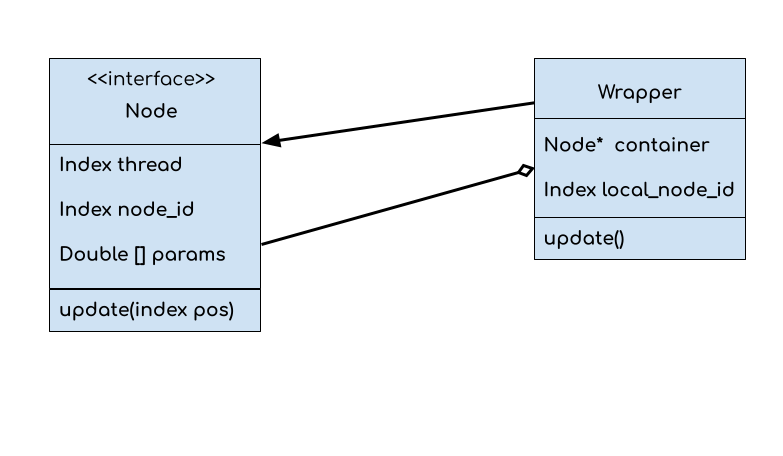
\includegraphics[width=0.6\textwidth]{src/pic/wrapper.png}
\caption{The naive solution for vectorization: The \texttt{Node} class in the NestKernel is adjusted by extending all its functions by a new parameter indicating the local ID of the node that we want to apply the function to. Additionally, the attributes in the \texttt{Node} class are modified to have a vector from. The \texttt{Wrapper} class inherits from the \texttt{Node} class and at the same time has an attribute with a \texttt{Node} type, which leads to a circular dependency and invalidates the whole design.}
\label{fig:naive}
\end{figure}

A direct naive solution to integrate vectorization into the NestKernel would be to replace all data fields in the \texttt{Node} base class and its derived classes with \texttt{vector<double>} instead of having single \texttt{double} attributes. With the current function signatures in the \texttt{Node} class, this would, however, mean that we could not update or inspect the state of the single instances individually and would have to extend the signature of these functions with a new parameter indicating the index into the vectors. Using this approach we then have the problem that we are missing the \emph{context}, meaning that when calling the \texttt{update()} or \texttt{get\_status()} functions in the NestKernel, we do not know which entries to update because the \texttt{Node} class would now represent a collection of nodes. To solve this issue, we would need an \emph{intermediate} class (called \texttt{Wrapper} in the following description) that has a \emph{pointer} to the \texttt{Node} class, and as a class member of the \texttt{Wrapper}, we could add an attribute representing the local ID of the node as the position of the entry in the \texttt{Node} class. In order to let the \texttt{Wrapper} class communicate with the other NestKernel components it would have to inherit from the \texttt{Node} class.

\autoref{fig:naive} shows the relation between the \texttt{Node} and \texttt{Wrapper} classes. The main problem of this design is a cyclic dependency between the \texttt{Wrapper} and the \texttt{Node} class, as the \texttt{Wrapper} inherits from the node and at the same time stores an instance of the \texttt{Node} class, which forces us to change the signature of the functions in the \texttt{Node} class and makes the \texttt{Wrapper} have twice the number of functions as the \texttt{Node} class does, because it needs an additional version of each function in the base class with the local ID as an additional parameter. Due to these conceptual flaws, we abandoned this design and developed a more robust solution, which will be explained in the next section.

\section{The Container}

To solve the issues of the naive solution, we have to clearly separate vectorized models from the already existing (non-vectorized) models. Node retrievals and updates should be performed in blocks and in parallel without dependencies between the nodes. Additionally, we have to avoid changing the declaration of the \texttt{Node} class functions to avoid the overhead of propagating these changes to the other derived classes from the \texttt{Node} class and make the implementation of the vectorized models transparent to the NestKernel components.

\begin{figure}[h!]
\centering
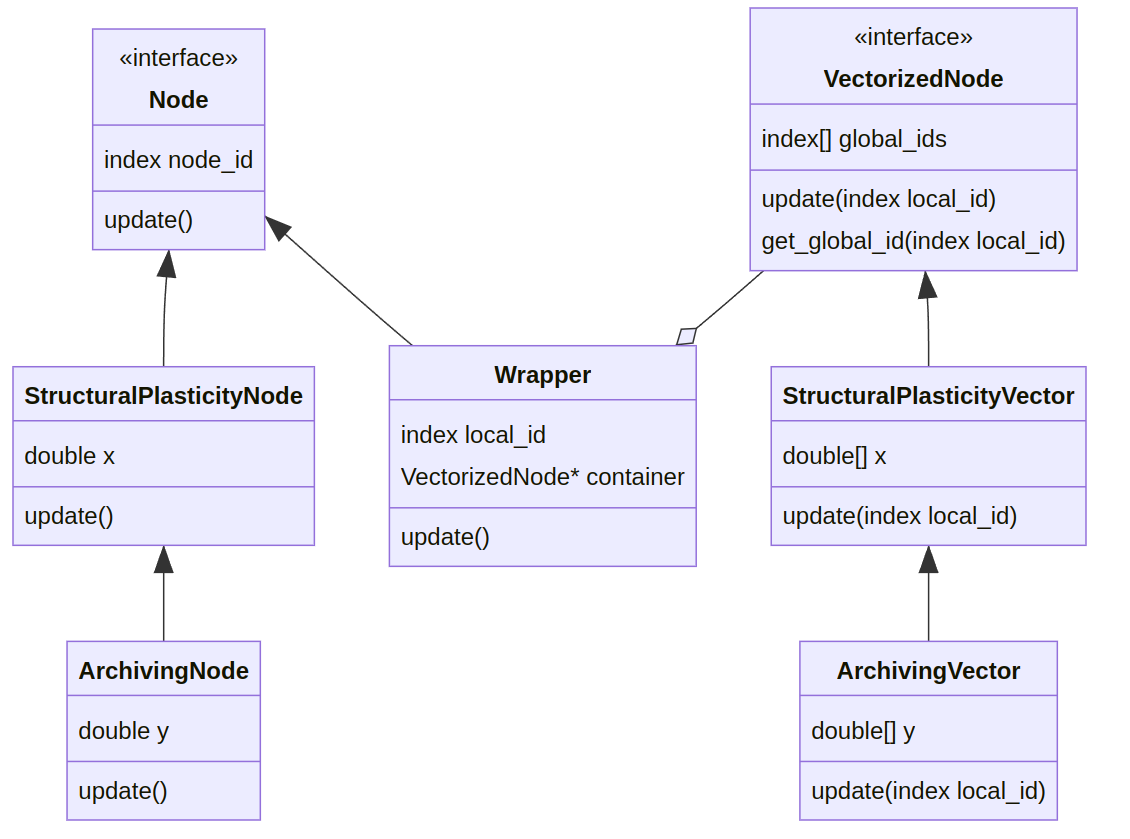
\includegraphics[width=0.8\textwidth]{src/pic/wrapper_node.png}
\caption{The \texttt{Wrapper} and the \texttt{VectorizedNode}: As in the naive implementation, the \texttt{Wrapper} still inherits from the \texttt{Node} interface, but instead of owning an attribute of the \texttt{Node} class, it owns an attribute of the \texttt{VectorizedNode}. The \texttt{VectorizedNode} class is a twin of the \texttt{Node} class, with the only difference that it supports vectorization.}
\label{fig:container}
\end{figure}

In \autoref{fig:container}, we illustrate the new solution that is derived from the naive solution. The idea behind this solution is to split the \texttt{Wrapper} from the naive solution into two different classes. The new \texttt{Wrapper} class inherits from the \texttt{Node} class, and has a member variable of type \texttt{VectorizedNode}. The \texttt{VectorizedNode} is an interface that has the same exact functionality as the \texttt{Node} interface, with the only difference that all its member variables are vectors and all functions have an extra parameter which represents the position of the entry that we want to retrieve or update. Instead of having $n$ instances of the \texttt{Node} class from any arbitrary model, we have a single container instance of the \texttt{VectorizedNode} that has vectors of size $n$ and each of these entries are represented by the \emph{Wrapper}. Since the \texttt{Wrapper} inherits from the \texttt{Node} class, the other components in the NestKernel can interact with the \texttt{Wrapper} without any further adjustments. Each call to the functions inside the \texttt{Wrapper} are forwarded to the \texttt{VectorizedNode} that calls the corresponding function with the local ID as the context given by the \texttt{Wrapper} instance. It is also important to note here that for each of \texttt{StructuralPlasticitiyNode} and the \texttt{ArchivingNode} we have equivalent vectorized classes derived from the \texttt{VectorizedNode} and which have the same functions as the original classes, but with support for vectorized models.

\begin{figure}[h!]
\centering
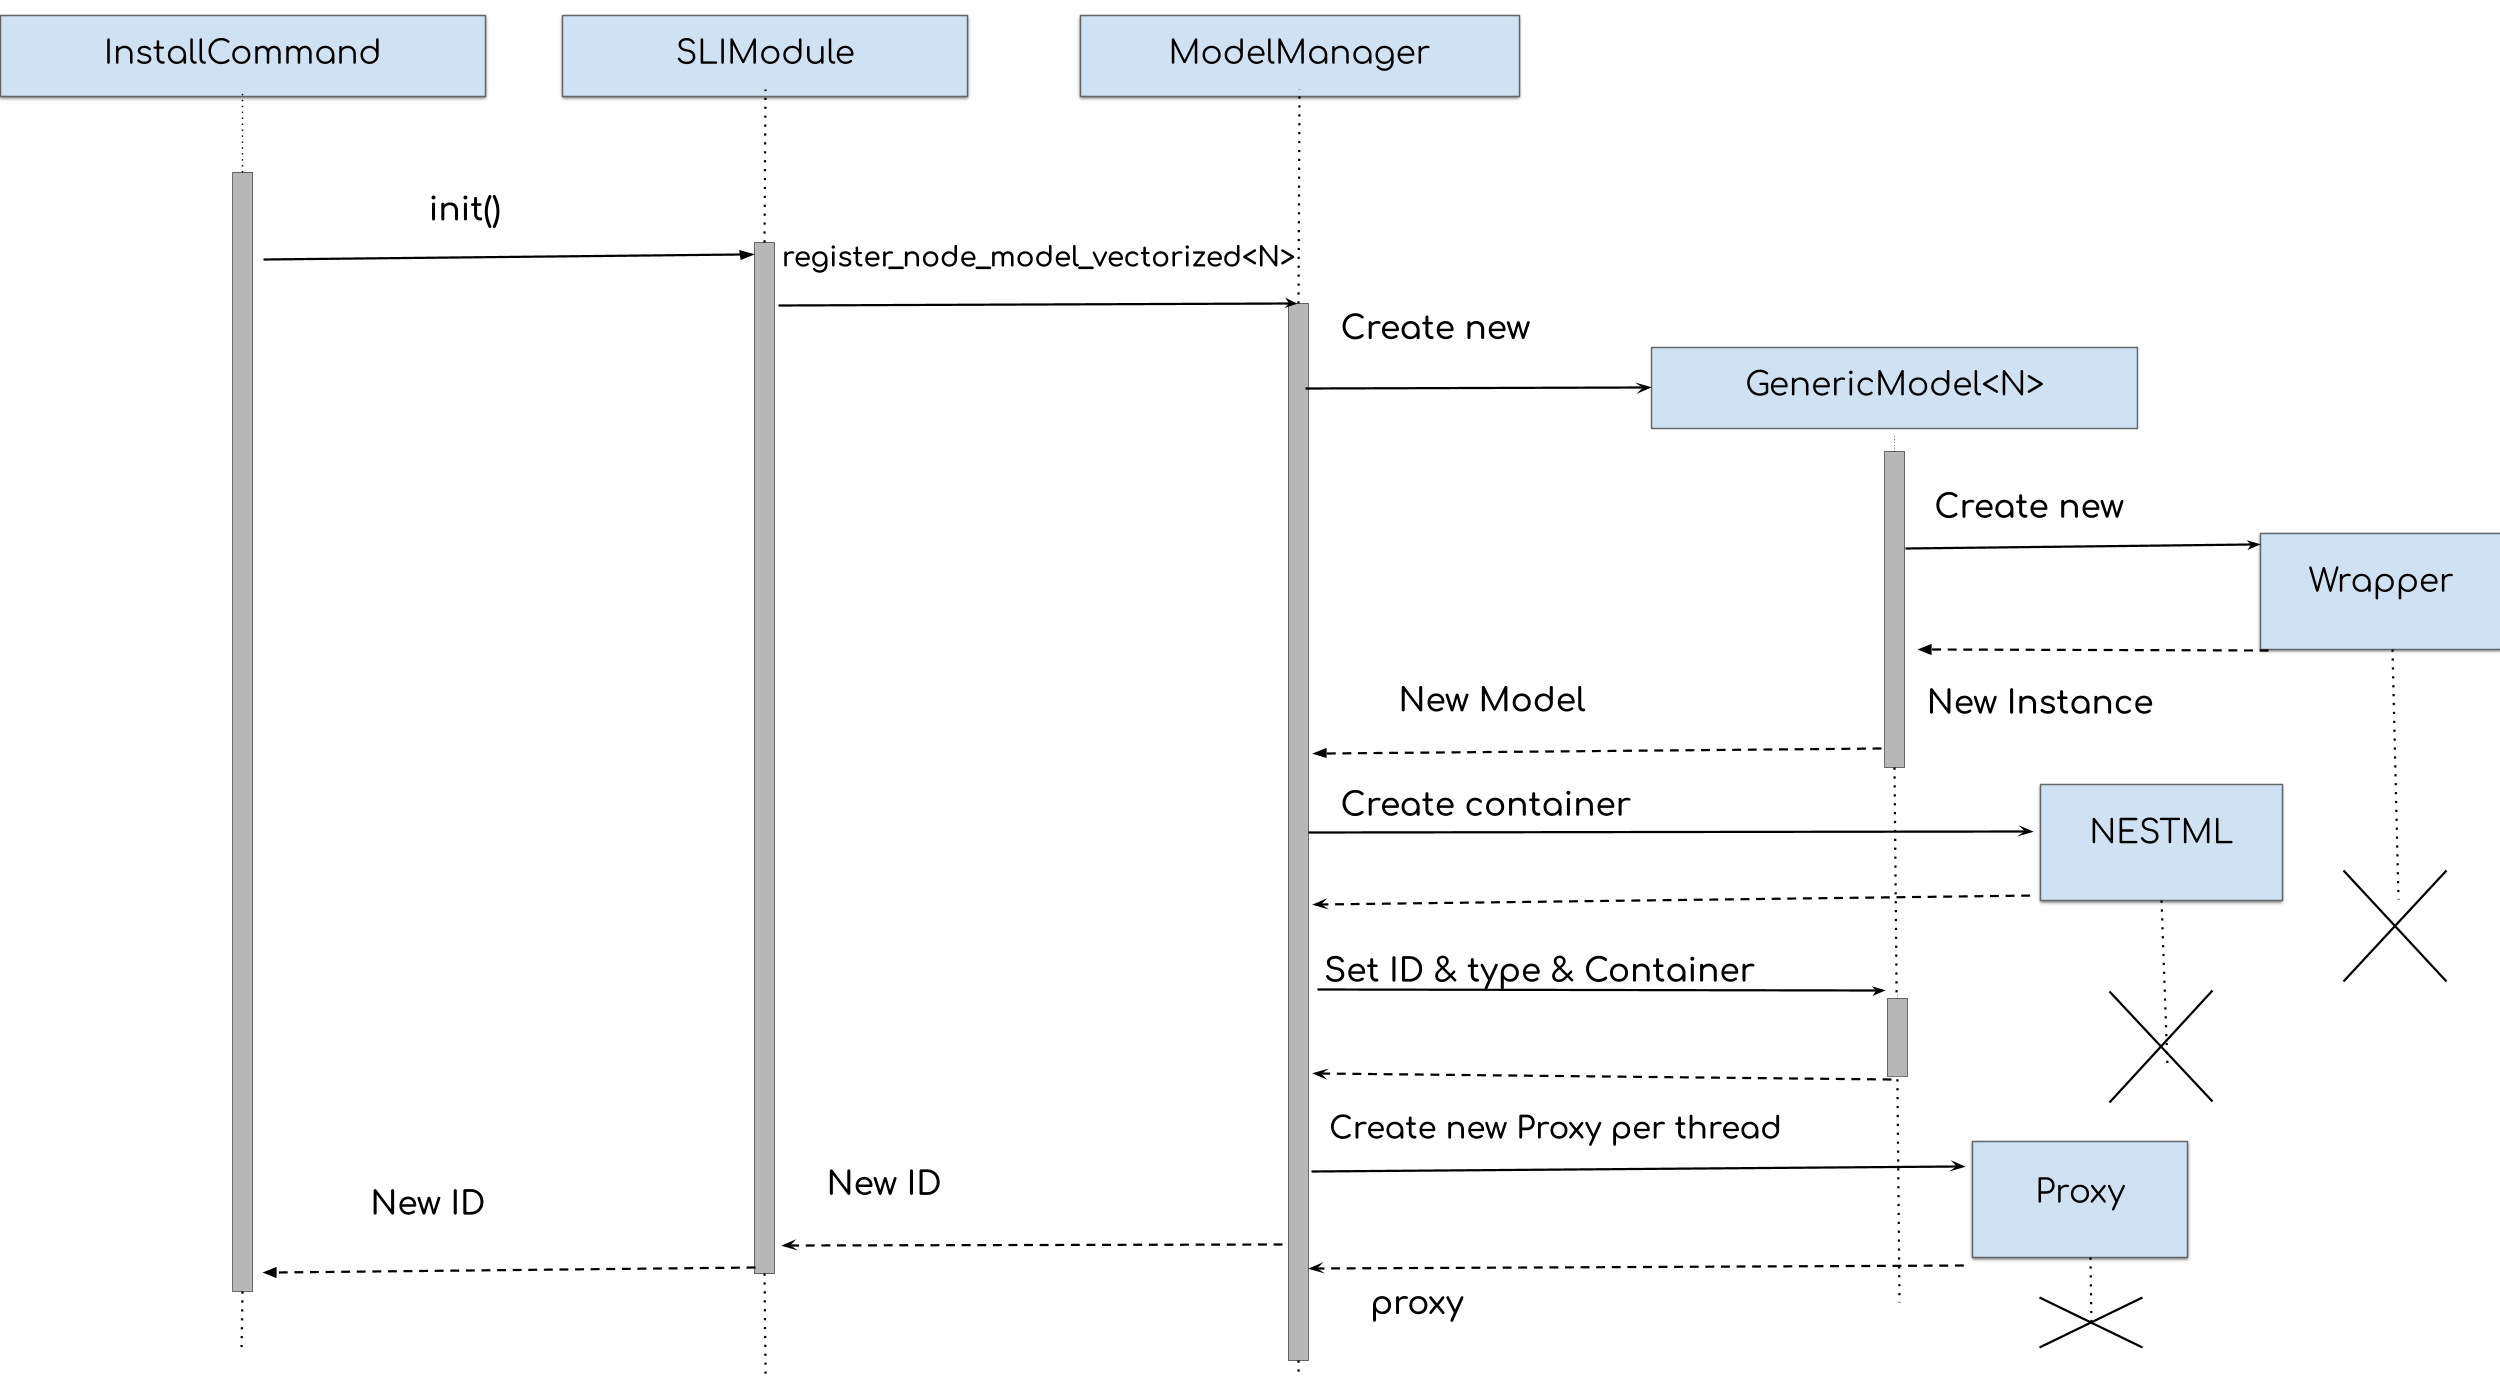
\includegraphics[width=\textwidth]{src/pic/node_creation_vec.png}
\caption{Registering a vectorized model: The message sequence chart depicts the interaction between the components in the NestKernel responsible for registering new custom vectorized models.}
\label{fig:register_container}
\end{figure}

As depicted in the \autoref{fig:register_container}, registering new external models in the NestKernel starts with calling the \texttt{register\_node\_model\_vectorized()} function in the \texttt{ModelManager}. The function then creates a new instance of the \texttt{GenericModel}, but instead of providing the model class type as the value of the template \texttt{T}, we set \texttt{T} to the \texttt{Wrapper}. In other words, we create an instance of type \texttt{GenericModel<Wrapper>}, which internally stores an instance of the \texttt{Wrapper}. After the constructor of the \texttt{GenericModel} finishes, the control returns to \texttt{register\_node\_model\_vectorized()}, which proceeds by creating an instance of the \texttt{VectorizedNode} which is indicated as \texttt{NESTML} in the figure. We create the container from the \texttt{VectorizedNode} and then update the created model by setting its \texttt{id}, \texttt{type} and \texttt{container}. Afterwards, as in the normal registration workflow, we create the \texttt{roxy} models for each thread. The main difference between registering a normal model and a vectorized model is thus in the class type \texttt{T} provided to the \texttt{GenericModel} and the extra step of creating the container as an instance of the \texttt{VectorizedNode} class.

In a typical simulation with external simple models without the vectorization feature, there is am important condition that must be satisfied between the created nodes and the current number of used threads. The condition states that each node exactly belongs to one thread and threads can not modify the state of nodes coming from different threads. Since the \texttt{VectorizedNode} behaves the same as the \texttt{Node} class, the same must hold for containers. Each container must belong exactly to one thread, and threads can only modify the containers they possess. In order for the \texttt{VectorizedNode} to fulfill this requirement, we have slightly modified the \texttt{Model} class and the  \texttt{add\_neurons()} function of the \texttt{ModelManager}.\\

\begin{figure}[ht!]
    \centering
    \lstset{language=C++,
                keywordstyle=\color{blue},
                stringstyle=\color{red},
                commentstyle=\color{green},
                morecomment=[l][\color{magenta}]{\#}
}
\begin{lstlisting}[caption=Assigning containers to threads,frame=tlrb, label=lst:thread_container]{Name}
 if ( model.get_uses_vectors() )
      {
        if ( model.has_thread_assigned( t ) )
        {
          index t_container_pos = model.get_node_pos_in_thread( t );
          t_container = vectorized_nodes.at( t ).at( t_container_pos );
        }
        else
        {
          t_container = model.get_container()->clone();
          t_container->set_thread( t );
          vectorized_nodes.at( t ).push_back( t_container );
          index t_container_pos = vectorized_nodes.at( t ).size() - 1;
          model.add_thread_node_pair( t, t_container_pos );
        }
      }
\end{lstlisting}
\end{figure}

\autoref{lst:thread_container} shows the inserted functionality in the \texttt{add\_neurons()} function for creating new \texttt{Node} instances from the registered models. We start by checking if the model class supports vectorization, and if this is the case, we ask the model instance if it has seen the current running thread $t$ or not. If the model knows thread $t$, an instance of the \texttt{VectorizedNode} was already created and we simply ask the model to give us the position of the container in the thread $t$ and retrieve it in order to resize and adjust it accordingly. If the model has not seen the $t$ yet, we \emph{clone} the container that is stored inside the model and update it by providing the thread $t$ that is owning it and also insert the container into the thread context. To simplify the matching between containers and threads, we have an attribute called \texttt{vectorized\_nodes} in the shape of \texttt{vector<vector<VectorizedNode>>}, so that the first dimension is occupied with the thread ID and the second dimension with the created containers. The created container $c$ within the thread $t$ is then stored as \texttt{vectorized\_nodes.at(t).push(c)}, and the thread is registered in the container by simply calling \texttt{container.set\_thread(t)}. Once the matching between the container and the thread is completed, we register the thread $t$ in the model instance, so that by the next call the model knows which container to retrieve at which position.

For models that do not support vectorization, the inserted block is ignored and the function \texttt{add\_neurons()}  continues to execute without further changes. Since the \texttt{Wrapper} inherits from the \texttt{Node} class, the \texttt{create()} function inside the model always returns an instance from the provided class \texttt{T} inside the \texttt{GenericModel<T>} class, which can be either the registered model without vectorization or the new \texttt{Wrapper} class. As depicted in \autoref{lst:creating_nodes_while}, we only have minimal changes within the \texttt{while-loop}, and update the container once after the loop to avoid the overhead of repeatedly calling \texttt{resize()} on it.\\

\begin{figure}
    \lstset{language=C++,
                keywordstyle=\color{blue},
                stringstyle=\color{red},
                commentstyle=\color{green},
                morecomment=[l][\color{magenta}]{\#}
            }
\begin{lstlisting}[caption=Creating nodes,frame=tlrb, label=lst:creating_nodes_while]{Name}
 while ( node_id <= max_node_id )
      {
        Node* node = model.create( t );

        node->set_container( t_container );
        node->set_node_id_( node_id );
        node->set_nc_( nc_ptr );
        node->set_model_id( model.get_model_id() );
        node->set_thread( t );
        node->set_vp( vp );
        node->set_initialized();

        local_nodes_[ t ].add_local_node( *node );

        node_id += num_vps;
        has_at_leat_one_node = true;
      }

      local_nodes_[ t ].set_max_node_id( max_node_id );
      if ( t_container and has_at_leat_one_node )
      {
        t_container->resize( max_new_per_thread, t );
      }
    }
\end{lstlisting}
\end{figure}

\section{Limitations}

So far, we only made vectorization work with \emph{multithreading}, and a full integration into the NestKernel is still pending. We have implemented the \texttt{VectorizedNode} class that represents a container holding vectors, and the size of these vectors is the number of created \texttt{Wrapper} instances pointing to the container. For simplicity, we can consider the container as an \emph{array} and the \texttt{Wrapper} instances represent each entry in the array. Thus, each \texttt{Wrapper} can only modify the entry it is pointing to. Right now, when we update the \texttt{Node} instances, we are iterating over each of them individually. For the normal models without vectorization, we can not do anything different, but for the vectorized models, we should aggregate the \texttt{Node} (i.e., \texttt{Wrapper}) instances that share the same container and then only apply the function we want on the container. Assuming we have $n$ containers and each container has $k$ \texttt{Wrapper}s pointing to it, and we have a function $f$ that is applied to these items separately the function will be called $n\cdot k$ times in total, and for a large $k$ this might be a huge overhead. Instead, we could aggregate the items and only call the function $f$ $n$ times. Thus, each container can fully utilize the vectorization by internally applying the function $f$ in parallel to the $k$ items.

In addition, the \texttt{get\_status()} and \texttt{set\_status()} functions do not fully utilize the implemented new data structure for vectorization. Assuming the container has $n$ vectors of size $k$ ($k$ is the number of attributes in the model). The normal execution of these functions takes each \texttt{Node} instance individually and iterates over the $k$ attributes and returns a \emph{dictionary} containing the values of the $k$ attributes. This workflow does not work well with vectorization, because if each \texttt{Wrapper} within the same container executes the same logic, then we might have a high number of cache misses. Assuming we have two consecutive accesses $x_i$ and $x_{i+1}$, and we have $k$ large enough so that not all vectors can be loaded into the registers, the \texttt{Wrapper} at position $x_i$ loads its necessary data and returns the dictionary, the second \texttt{Wrapper} $x_{i+1}$ on the other hand must load the first $k$ vectors again. What really should happen is that each of the $l$ vectors must be loaded once in the registers. Since we have a consecutive access, all the entries must be loaded and ready to be used for constructing the result. Better yet, we could again group the \texttt{Wrapper} instances by the container type and let the container call these functions and treat each of these $k$ vectors individually and in parallel.

\cleardoublepage

\chapter{Performance}
 \label{chap:perf}
 
 The major goal of this work is to have a fully automated model generation in PyNEST without drastically degrading the performance of the simulation script and encouraging users to use the new implemented JIT module. In order to test the impact of the using the JIT module in the simulation script, we need to test different configurations that might eventually appear when running the simulation with JIT. Firstly, we test the neuronal network with the script explicitly calling PyNESTML module and the \texttt{nest.Install} function and  consider its running time as our base model. Secondly, we run the same neuronal network, but this time everything is controlled by the JIT module. Thirdly, we repeat the same experiment, but this time we choose a neuronal network that includes using a custom implemented synapse.
 
 As the NestKernel does not completely utilize the new data structure behind vectorization, we can not really make meaningful evaluation of its impact on the performance. Therefore, we only decided to compare single functions between simple and vectorized models. Such functions are \texttt{nest.Create} and \texttt{nest.GetStatus}.
 
 From the JIT tool perspective, we do not really care about the size of the network or its behave, because we only simply retrieve the model and make it available to the simulation script. In that case, any neuronal network should be fine to test with. In the first experiment, we choose a random balanced network as  described by \emph{Brunel} \citep{brunel2000dynamics}. For the second experiment with synapse, we build a network with a spike-timing dependent plasticity (STDP) synaptic type.
 
 
 For vectorization, we only test the \texttt{nest.Create} and \texttt{nest.GetStatus} functions by creating instances of the \emph{Izhikevich} \citep{1257420} with modifying the number of instances and the number of used threads.
 
\section{The JIT Module}

\subsection*{Running The JIT Module Without An external Synapse Type}

In the first experiment in testing the JIT module, we run the \emph{Brunel} network by explicitly using the PyNESTML to generate the code for the required model, and then we run the same network by using the JIT module. The result of the experiment can be found in the \autoref{fig:max_average_min}.

\begin{figure}[ht!]
    \centering
    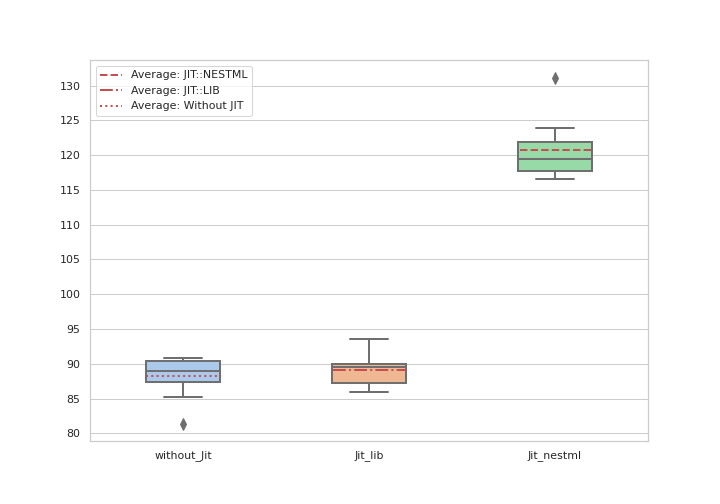
\includegraphics[width=\textwidth]{src/pic/box_plot_three.png}
    \caption{Network with custom neuron and built-in synapse: The blue box represents the performance of the simulation script without using JIT, and it has the best performance among the other experiments. The orange box represents the performance of running the same neural network with JIT but with the model being an external model being already built in a dynamic library. Finally, the green box is for running the simulation with JIT, but the neuron model is only available in a NESTML file format. The red lines inside each box represent the average runtime of the experiments.}
    \label{fig:max_average_min}
\end{figure}

In the \autoref{fig:max_average_min}, we show the runtime of three possible cases. The first is when we are explicitly calling the PyNESTML module, and it is labeled with \emph{Without\_Jit}. The second case is when running the simulation with an external model using the JIT module, and it is labeled with \emph{Jit\_Nestml}. The last case is when using JIT with an external library, and usually it is the result after generating the code for the \emph{nestml} model. The last case is labeled with \emph{Jit\_Lib} in the plot. In each of the three cases, we show the \emph{maximum}, \emph{average} and \emph{minimum} required to run the simulation.

The first case (i.e., \emph{Without\_Jit}) has the lowest runtime, and it took on average 90 seconds to finish the simulation. In the other hand, the average runtime for the \emph{Jit\_Nestml} took around 130 seconds, and the \emph{Jit\_Lib} took around 90 seconds.  Both the first case and the last case have almost the same behavior, with the exception that the \emph{minimum} runtime for the last case was a bit higher. This can be explained with the introduced overhead in the JIT module, and it is most significant in the second case. All the three values of the \emph{Jit\_Nestml} are the highest among the other cases, and it can be explained by the time required for searching the model and maintaining \texttt{NodeCollectionProxy} by converting the \texttt{JitNodeCollection} to the real \texttt{NodeCollection} instances and copying the parameters from one instance to the other.


\subsection*{Running The JIT Module with An external Synapse Type}

In the second experiment, we ran the \emph{STDP windows} simulation script from the \texttt{NESTML} tutorial, and again we compared the simulation runtime with using the JIT module against the original script. In this tutorial, we have a function that is responsible for creating the instances of the models and creating the network, and it is called multiple times in a \emph{for-loop} (exactly 151 times). In the JIT tool settings, it means that the model will be searched many times, and we would expect that only the first iteration will take most of the time in comparison to the subsequent iterations. 

\begin{figure}[ht!]
    \centering
    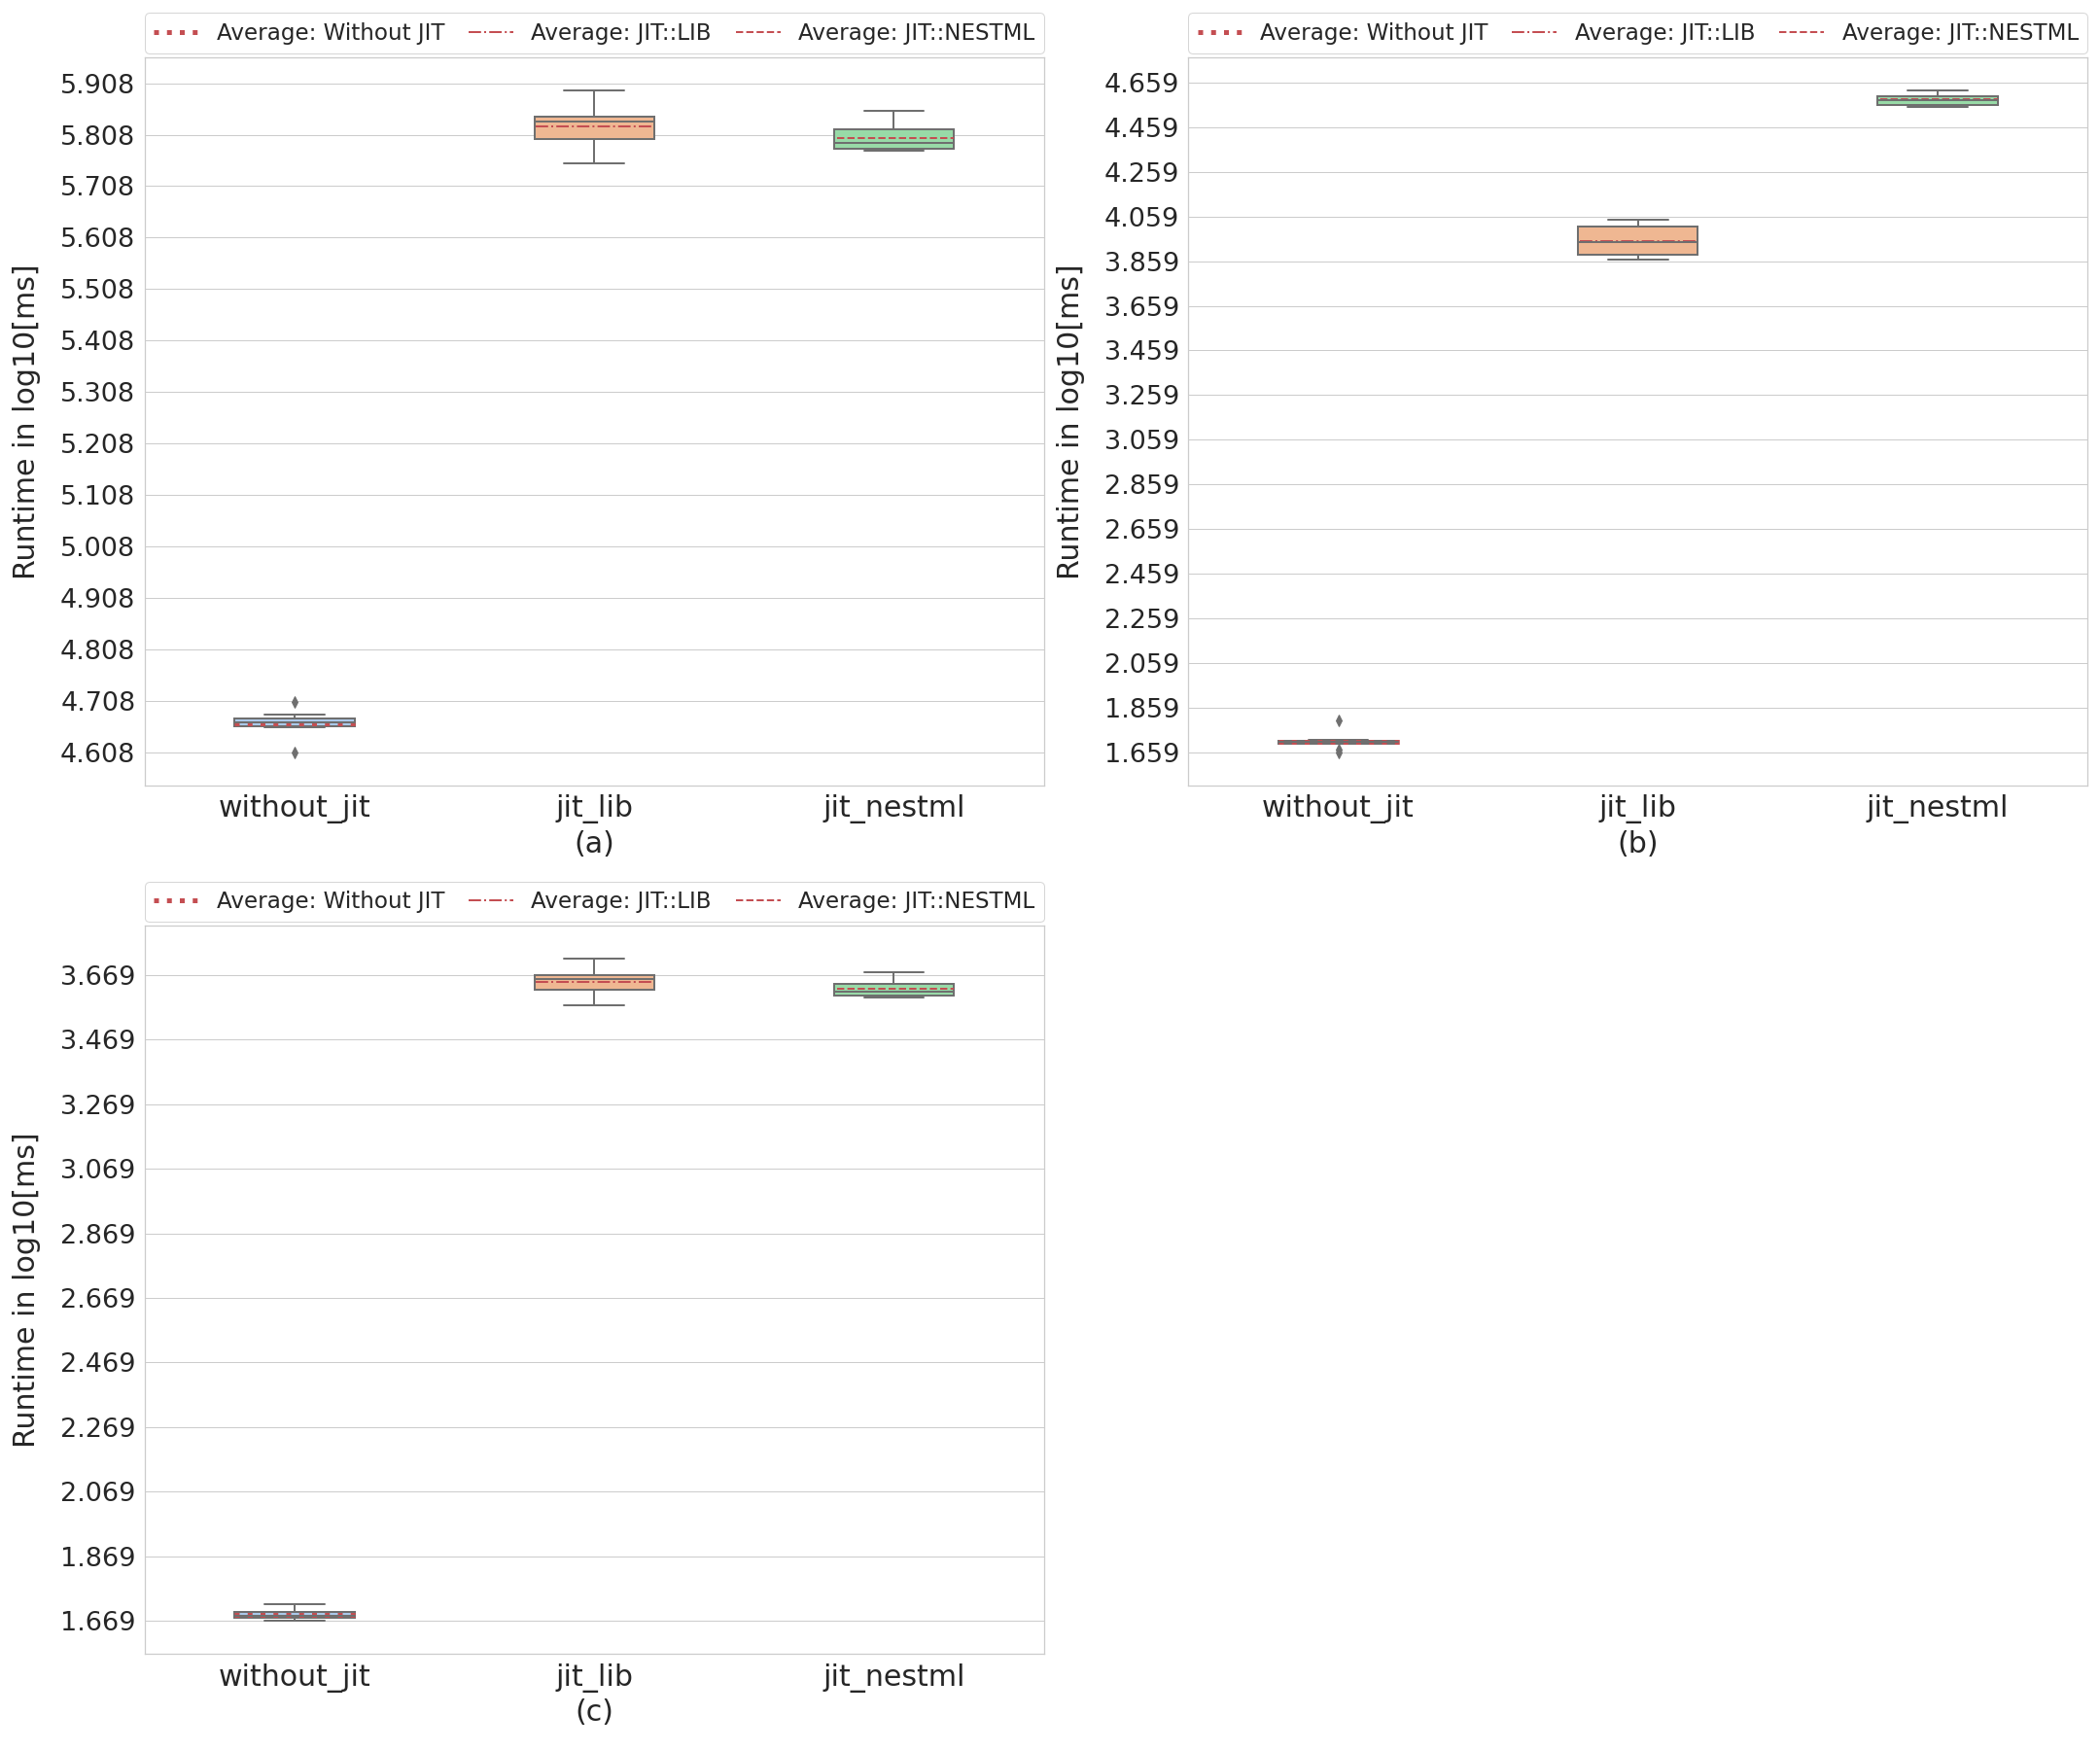
\includegraphics[width=\textwidth]{src/pic/three_plots.png}
    \caption{Network with custom neuron and built-in synapse: The first plot \emph{a} represents the overall runtime of the three experiments. The second plot \emph{b} shows the average runtime of the first iteration in all the three experiments. In the last plot \emph{c}, we compute the average runtime for all iterations for each run and then take the average runtime over the multiple runs. }
    \label{fig:overall_runtime}
\end{figure}

In the \autoref{fig:overall_runtime}, we analyze the runtime of the whole script, and then we take a look at the runtime of the function responsible for creating the network in each iteration. At the top left in the figure, we can observe the significant effect of using the JIT module with an external synapse type.  The JIT module requires on average more 700 seconds, whereas the normal execution took around 50 seconds to finish. The minimum runtime of the JIT approach is also very high in comparison to the normal mode. If we observe the second plot at the top, we can straightforward see the reason behind the 700-second runtime. The first iteration alone took more than 40 second to finish, whereas the normal execution took less than one second to finish. This difference is caused by the same overhead discussed above, plus now we have to  trigger the code generation pipeline again and replace the \emph{source/target} elements in the network with the new correct neuron model and update its state along the synapse instance. 

In the third plot at the bottom left of the figure, we show the average time needed by all the 151 iterations in each run. As expected, the result shows that mostly only the first iteration takes the longest running time. The average is around 4.5, and it is way smaller than the average of running the first iteration. The results seem to be consistent as we have $4.5 \times 151$ is around 700 seconds. On the other hand, the average runtime of the 151 iterations without the JIT module is significantly lower. As the external models will be available after the first iteration, which is the main reason why the left bottom plot shows better runtime than the first iteration, we still have the overhead of going through the \texttt{Wrapper} to execute the PyNEST functions, which introduces a great overhead.



\section{Vectoriztation}

As NestKernel does not completely support \emph	{vectorization} yet, we restrict our tests to the direct functions involved with the vectorized the model. We tested both the \texttt{nest.Create} and \texttt{nest.GetStatus} functions. Both experiments share the same configuration, we mainly can either change the number of created nodes and keep the number of threads constant or vice-versa. The experiments are executed with a \emph{Ryzen 7 3700u} processor with four cores and eight threads.
For the number of the nodes, we have picked \{1, 10, 30, 50,100,300,500,2000,5000,8000,1000\} and for the threads we have \{1, 2, 4, 8, 16, 32\}. Each sub-experiment is run five times, with storing the \emph{Wall} time in a \emph{csv} file containing the runtime of the vectorized and \emph{non-vectorized} model. In each sub-experiment, we have three plots. In the first plot on the left, we show the \emph{max-average-min} runtime of the vectorized model. The middle plot shows the \emph{max-average-min} runtime of the simple \emph{non-vectorized} model. Finlay, the last plot on the most right, overlays the average runtime for both models in a single plot. The \emph{y-axis} in the first two plots shows the values after applying the \emph{logarithmic} function with base 10 on the runtime values, which were stored in microseconds, whereas the values in the last plot are only in microseconds.

\subsubsection{The Create function}

\subsubsection*{Varying the number of nodes with a constant number of threads}

 In the first configuration in testing the \texttt{nest.Create} function, we fix the number of threads and vary the number of nodes. In the  \autoref{fig:threads_1} until \autoref{fig:threads_32}, we show the results of the experiments. For each number of threads, we display the performance of the \texttt{nest.Create} function with the vectorized model against the simple models. 


In the \autoref{fig:threads_1}, we observe that both types of models behave the same until reaching a number of nodes larger than 300 ($10^{2.5}$). After that point, the vectorized model starts to become a bit slower on average, but with few microseconds. Another observation is that the min-max area of the vectorized model is a bit fat and gets more narrow after reaching $10^3$, whereas the min-max area is almost always narrow, and it gets more narrow after reaching 300 nodes.

In the \autoref{fig:threads_2}, we observe the same performance for both types of models, even the \emph{max-min} area looks almost the same. As in the previous experience, the performance of the vectorized model becomes a bit slower after reaching 300 nodes with a few milliseconds in comparison to the simple model. In  \autoref{fig:threads_4} with four threads, we have the same observation as in the  \autoref{fig:threads_2} with two threads.

In the rest of the figures with threads in \{8, 16, 32\}, we observe that the vectorized model gets slower and the gap between both models gets wider but still in the range of a few milliseconds.

\begin{figure}[ht!]
    \centering
    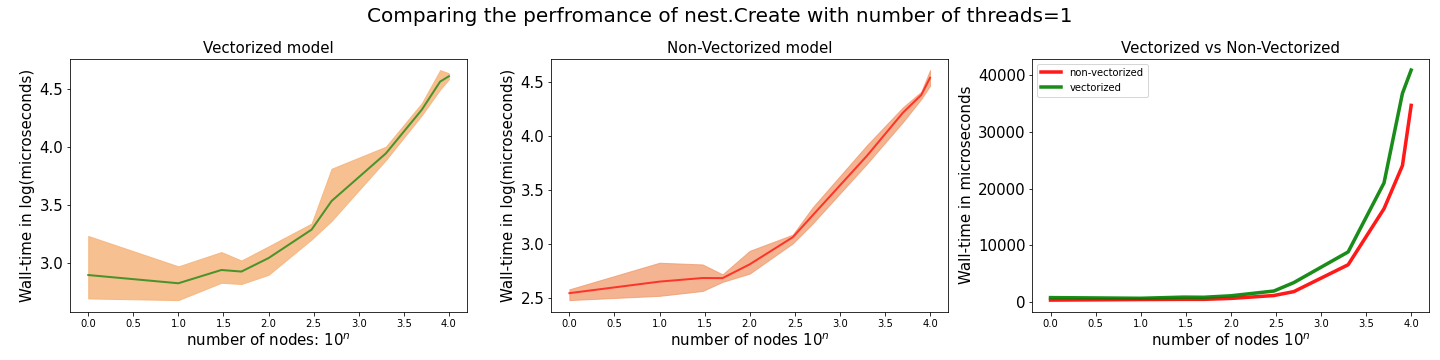
\includegraphics[width=\textwidth]{src/pic/thread_1.png}
    \caption{Performance of \texttt{nest.Create} function with the number of $threads=1$: The left plot depicts the average performance of the vectorized model. The plot in the model shows the average performance of the original non-vectorized model in NEST. The last plot in the right overlays the average performance of both models. Additionally, in the first two plots in the left, we show the min-max area, and it is depicted in orange and red respectively.}
    \label{fig:threads_1}
\end{figure}

\begin{figure}[ht!]
    \centering
    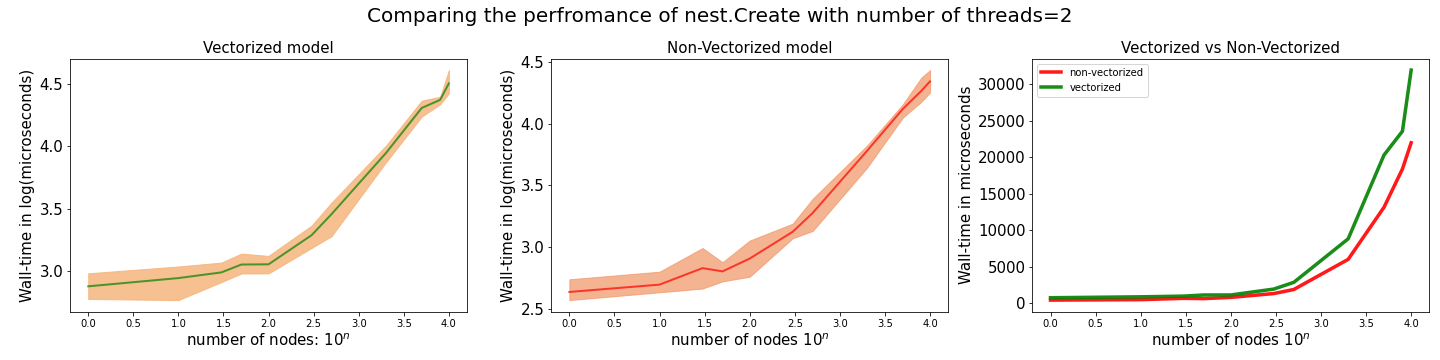
\includegraphics[width=\textwidth]{src/pic/thread_2.png}
    \caption{Performance of \texttt{nest.Create} function with the number of $threads=2$: The left plot depicts the average performance of the vectorized model. The plot in the model shows the average performance of the original non-vectorized model in NEST. The last plot in the right overlays the average performance of both models. Additionally, in the first two plots in the left, we show the min-max area, and it is depicted in orange and red respectively.}
    \label{fig:threads_2}
\end{figure}

\begin{figure}[ht!]
    \centering
    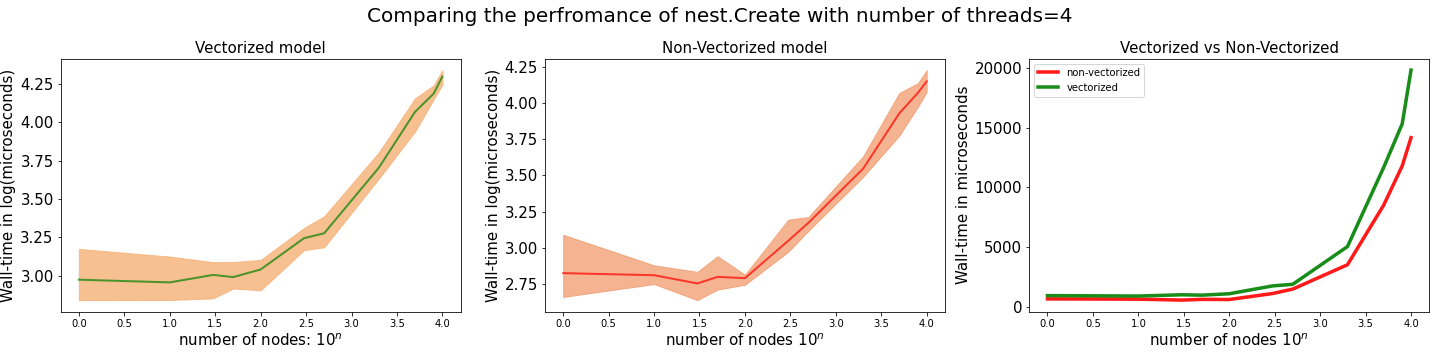
\includegraphics[width=\textwidth]{src/pic/thread_4.png}
    \caption{Performance of \texttt{nest.Create} function with the number of $threads=4$: The left plot depicts the average performance of the vectorized model. The plot in the model shows the average performance of the original non-vectorized model in NEST. The last plot in the right overlays the average performance of both models. Additionally, in the first two plots in the left, we show the min-max area, and it is depicted in orange and red respectively.}
    \label{fig:threads_4}
\end{figure}

\begin{figure}[ht!]
    \centering
    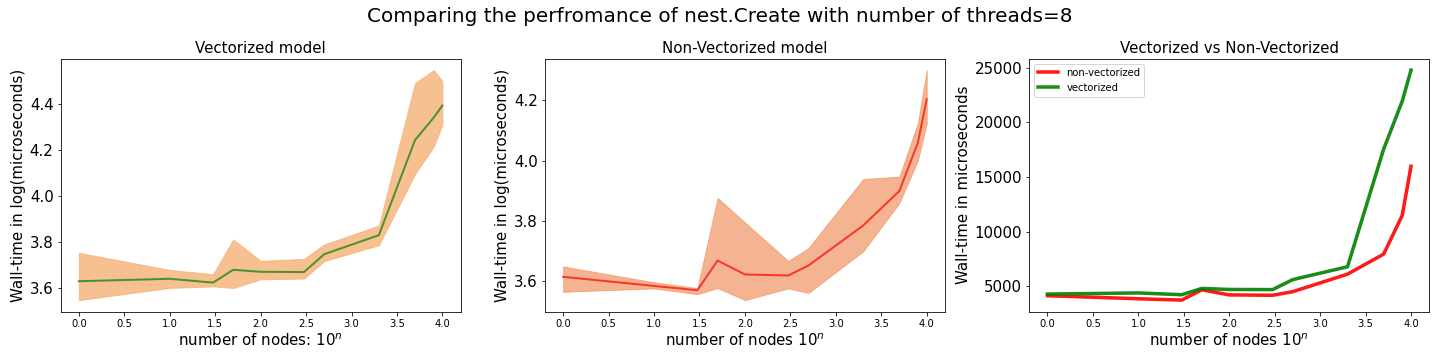
\includegraphics[width=\textwidth]{src/pic/thread_8.png}
    \caption{Performance of \texttt{nest.Create} function with the number of $threads=8$: The left plot depicts the average performance of the vectorized model. The plot in the model shows the average performance of the original non-vectorized model in NEST. The last plot in the right overlays the average performance of both models. Additionally, in the first two plots in the left, we show the min-max area, and it is depicted in orange and red respectively.}
    \label{fig:threads_8}
\end{figure}


\begin{figure}[ht!]
    \centering
    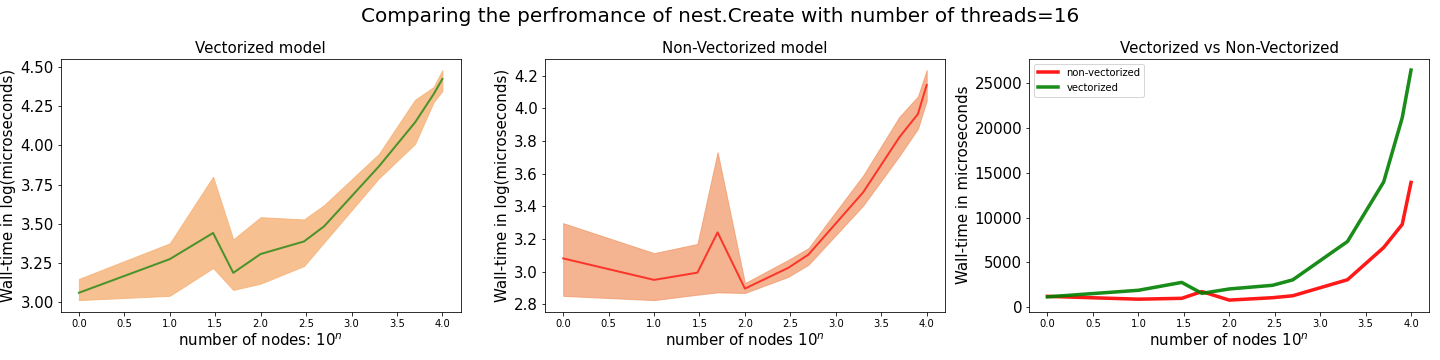
\includegraphics[width=\textwidth]{src/pic/thread_16.png}
    \caption{Performance of \texttt{nest.Create} function with the number of $threads=16$: The left plot depicts the average performance of the vectorized model. The plot in the model shows the average performance of the original non-vectorized model in NEST. The last plot in the right overlays the average performance of both models. Additionally, in the first two plots in the left, we show the min-max area, and it is depicted in orange and red respectively.}
    \label{fig:threads_16}
\end{figure}

\begin{figure}[ht!]
    \centering
    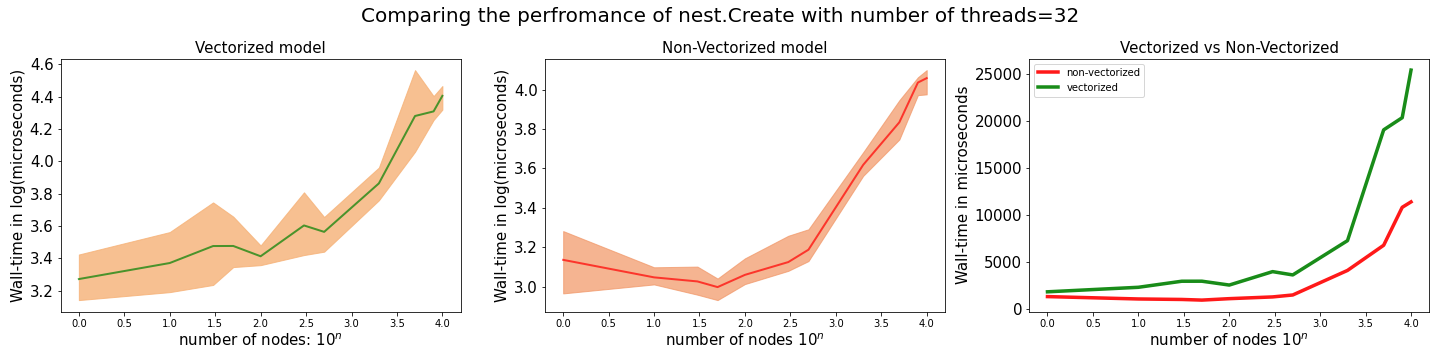
\includegraphics[width=\textwidth]{src/pic/thread_32.png}
    \caption{Performance of \texttt{nest.Create} function with the number of $threads=32$: The left plot depicts the average performance of the vectorized model. The plot in the model shows the average performance of the original non-vectorized model in NEST. The last plot in the right overlays the average performance of both models. Additionally, in the first two plots in the left, we show the min-max area, and it is depicted in orange and red respectively.}
    \label{fig:threads_32}
\end{figure}

\subsubsection*{Varying the number of threads with a constant number of nodes}


In general, the plots between the \autoref{fig:nodes_1} and \autoref{fig:nodes_10000} show that the \texttt{nest.Create} function has a consistent behavior. In all the plots, we can observe the discontinuity that happens around the points 4, 8 and 16. At these points the slope changes significantly, and the reason behind it is the processor specification. Recall that we ran the experiments on a four-core processor. In general, the vectorized model is a bit slower than the simple model and the largest difference can be observed in the \autoref{fig:nodes_5000} with 5000 nodes. Compared to the previous experiment with fixed number of threads, the min-max area seems to be more a bit fat, which might implicate that the current average results might be a bit noisy.

\foreach \n in {1, 10, 30, 50, 100, 300, 500, 2000, 5000, 8000, 10000}
{
\begin{figure}[ht!]
    \centering
    \includegraphics[width=\textwidth]{src/pic/nodes_\n.png}
    \caption{Performance of \texttt{nest.Create} function with the number of $nodes=$\n: The left plot depicts the average performance of the vectorized model. The plot in the model shows the average performance of the original non-vectorized model in NEST. The last plot in the right overlays the average performance of both models. Additionally, in the first two plots in the left, we show the min-max area, and it is depicted in orange and red respectively.}
    \label{fig:nodes_\n}
\end{figure}
}

\subsubsection{The GetStatus function}

\subsubsection*{Varying the number of nodes with a constant number of threads}

Even with the \texttt{nest.GetStatus} not fully being optimized to support vectorization, both the vectorized model and the simple one has the same performance, with the vectorized model being slightly better with few microseconds.

\foreach \n in {2, 4, 8, 16, 32}
{
\begin{figure}[ht!]
    \centering
    \includegraphics[width=\textwidth]{src/pic/get_thread_\n.png}
    \caption{Performance of \texttt{nest.GetStatus} function with the number of $nodes=$\n: The left plot depicts the average performance of the vectorized model. The plot in the model shows the average performance of the original non-vectorized model in NEST. The last plot in the right overlays the average performance of both models. Additionally, in the first two plots in the left, we show the min-max area, and it is depicted in orange and red respectively.}
    \label{fig:get_threads_\n}
\end{figure}
}

\subsubsection*{Varying the number of threads with a constant number of nodes}

The \texttt{nest.GetStatus} with varying the number of threads has a very different behavior. In the \autoref{fig:get_nodes_1}, both models have the same direction of variation with the only difference that at $threads=16$ we observe that the vectorized model is becoming a bit faster. The min-max area in both models is also almost the same. With the number of nodes equal to ten in \autoref{fig:get_nodes_10}, we observe that between the points 6 and 16 the vectorized model is significantly faster, but then starting from 16 the vectorized model becomes slower again. In both plots, the min-max area is very noisy.


In \autoref{fig:get_nodes_30}, both  models have the same behavior, with the vectorized model being a bit faster between the points 3 and  14 and then again after 20. Both min-max areas have almost the same shape. In \autoref{fig:get_nodes_50}, the average performance between the models is significantly different with 1500 microseconds on average. Again, we directly observe the points where the slope of the curves changes. Those points are at position 4, 8 and 16. \autoref{fig:get_nodes_30} with 100 nodes shows also the same observations as in the \autoref{fig:get_nodes_30}.

In \autoref{fig:get_nodes_300} with 300 nodes, the vectorized model takes almost completely the lead in all thread values, with the only exception between position 6 and 10. Both \autoref{fig:get_nodes_500} and \autoref{fig:get_nodes_2000} respectively with 500 and 2000 nodes show the same observations, where the vectorized model is being faster than the simple model.

Reaching higher number of nodes as in \autoref{fig:get_nodes_5000} with 5000 nodes in \autoref{fig:get_nodes_8000} with 8000 and in \autoref{fig:get_nodes_10000} with 10000 nodes, the vectorized model is either behaving the same as the simple model or performing even better.



\foreach \n in {1, 10, 30, 50, 100, 300, 500, 2000, 5000, 8000, 10000}
{
\begin{figure}[ht!]
    \includegraphics[width=\textwidth]{src/pic/get_nodes_\n.png}
    \caption{Performance of \texttt{nest.GetStatus} function with the number of $threads=$\n: The left plot depicts the average performance of the vectorized model. The plot in the model shows the average performance of the original non-vectorized model in NEST. The last plot in the right overlays the average performance of both models. Additionally, in the first two plots in the left, we show the min-max area, and it is depicted in orange and red respectively.}
    \label{fig:get_nodes_\n}
\end{figure}
}



\cleardoublepage

\chapter{Discussion}
 \label{chap:disc}
 \section{Conclusions and Summary}

The aim of the thesis was to eliminate the explicit calls to the NESTML interface in the simulation script. The eliminated calls are then replaced by an automated workflow controlled by the JIT mechanism running in the background. Two major components are built in the JIT mechanism to make it work seamlessly without having a great impact on the simulation script. The main component is the Wrapper class that is responsible for intercepting the function calls in the NESTML interface and by either delaying their executions or applying certain pre- and post-processing steps before or after the real function calls.

The second component is the NodeCollectionProxy. Intercepting the call to the \texttt{Create} function, we were able to create a partial version of the NESTML model that provides functionalities to retrieve and update the state of the instances before really being instantiated from the complete NESTML model. The role of the NodeCollectionProxy is to make the retrieve and update calls for the partial version of the model work exactly as the complete models without the user noticing these changes. 

Due to the existence of the of partial instances of the NESTML model in the Python level and the real complete instances of the model in the C++ level, we double the memory requirements of the simulation script. To abate the memory requirements, we adjust the internal model representation in the NestKernel by making the model independent of the storage of its properties. The adjusted new representation supports vectorization by grouping all instances of the same model into one central unit also called a vectorized model. The attributes of the vectorized model are in a vector form, and their size is equal to the number of instances created during the simulation of that particular
model type. Additionally, the vectorization opens up possibilities for future optimizations, such as decomposing the generated C++ code of the NESTML block into independent blocks and incrementally assembling the models during the evolution of the simulation.

In this chapter, we give an overview of the main concepts introduced in the previous chapters and discuss potential improvements that could benefit from bringing the JIT approach and vectorization closer to each other.

\subsection*{JIT Module: The Wrapper}

In \autoref{chap:jit} we have designed and implemented a wrapper around PyNEST, which can intercept function calls, and depending on specific constraints, can either apply some pre-processing and post-processing steps before calling the original function, or disable the original function completely. The wrapper has a straightforward structure that renders its use simple and flexible. Each targeted function in PyNEST has a custom wrapper, and these wrappers are registered in a dictionary\todo{never introduce new terms in the conclusion}, with the keys being the name of the targeted function and the values of the registered classes. Once the JIT module is imported, it iterates over PyNEST's high-level functions, methods, and classes, and if one of these objects is registered in the dictionary, a wrapper instance is created and inserted into the JIT module. Non-targeted objects are inserted directly without a wrapper in between. Another main feature of the wrappers is that they are implemented independently and do not influence each other.

\subsection{JIT Module: The lightweight version} \todo{be consistent with numbering and capitalization}

Since the implemented wrapper for the \texttt{Create()} function must search for the model, and in the worst case, the code of the models must be generated, we decided to split the code generation overhead. Upon a call to \texttt{Create()}, the user will not need to wait for the whole code of the model to be generated, built, and installed, but instead we create a \emph{lightweight} version of the model that only has the \emph{state} and \emph{parameter} blocks, but allows the user to parametrize it using deterministic or randomized values already before the full code is available. The real models will become available once the user calls the \texttt{Connect()} function.

One drawback with this approach is that after calling \texttt{Connect()} or \texttt{Simulate()} when the full models are available, the model attributes have to be copied from the lightweight version to the real instances, which leads to a duplication of memory, once on the Python level and once on the C++ level.

\subsection*{JIT Module: The NodeCollectionProxy}

In order to retrieve information from the lightweight version and make the handling of the code generation transparent and similar to PyNEST's \texttt{NodeCollection}, we have implemented the \texttt{JitNodeCollection} and the \texttt{NodeCollectionProxy}. The relation between these three elements is a tree structure, in which the \texttt{NodeCollectionProxy} is the root element. It has two children, the first being the \texttt{JitNodeCollection} and the second being the \texttt{NodeCollection}. The \texttt{JitNodeCollection} has an arbitrary number of children. If the IDs of the children of the \texttt{JitNodeCollection} build a contiguous space, and they belong to the same model, they are represented by the \texttt{JitNode}, which represents the leaves of the tree. The \texttt{NodeCollectionProxy}, the \texttt{JitNodeCollection} and the \texttt{JitNode} share the same interface that supports retrieving and setting the attributes of the instances as well as \emph{indexing} and \emph{slicing} exactly like the provided functionalities in the \texttt{NodeCollection}.

\subsection*{Vectorization}

To address the problem with memory duplication explained above, we have introduced a new data structure in the NestKernel for handling models. The new data structure is based on the idea of a \emph{structure of arrays (SoA)}, where instead of having $n$ instances of the same model with $k$ attributes, we have exactly one instance that has $k$ attributes in the form of \emph{vectors} and each of these vectors has a size of $n$. The vectorization of models behaves like a container of nodes, so instead of updating the nodes separately, we can now tell the containers to updates the states of all nodes in parallel by utilizing the efficiency of \emph{SIMD} instructions in modern processors. The vectorization should also decrease the amount of \emph{cache misses}, as updating a container exploits the spatial locality of the items in the array and thus requires fewer data transfers from main memory.

\subsection*{Performance}

The performance of the JIT module without using an external synapse model does not deviate a lot from running the simulation script without the JIT tool. However, when using an external custom synapse, we observe a significant difference \todo{decrease?} in the performance \todo{increase in runtime?}. The difference can be explained by the overhead of running some steps of the code generation pipeline twice, maintaining the functionality of the \texttt{NodeCollectionProxy} and finally replacing the network nodes and updating their parameters. The fact that the vectorization support in NestKernel is currently not leveraging the full potential is reflected by the fact that the performance of the \emph{vectorized} models and the \emph{non-vectorized} models are still quite similar on average.

\section{Outlook}

\subsection*{Modularity}

As mentioned multiple times already, the duplication of memory between the Python and C++ sides because of the lightweight version of the model is a severe problem that is only partially solved by the current vectorization strategy. Moreover, the current version of the \texttt{NodeCollectionProxy} requires that each change in PyNEST's \texttt{NodeCollection} must be followed which leads to an increased maintainance burden for the JIT project. To mitigate these problems, we can improve the concept of the lightweight version and make it more flexible by adjusting the code generation pipeline and making it generate and build the library in pieces. The model could, for example, be split into two pieces: The first would contain the state and parameters blocks, which could be generated and built upon the call to \texttt{Create()}. The remaining code could then be generated in the background and connected with the first part when calling the \texttt{Connect()} or \texttt{Simulate()} functions. Since the co-generation of the neuron and synapse just moves variables from the synapse to the neuron, we may then generate the code of the synapse and also split it into two parts: the first part would include the moved variables in a separate library and append them to the neuron state block during the simulation. The second part would take care of the rest of the functionality in the synapse and make it available during the \texttt{Connect()} call.

\subsection*{Removal of the NodeCollectionProxy}

With the extended \emph{modularity} as outlined above in place, we could completely drop the use of the current data structures required for the JIT mechanism (i.e., the \texttt{NodeCollectionProxy}, \texttt{JitNodeCollection} and \texttt{JitNode}). The NestKernel infrastructure would then be adjusted to support the modularity of the models and make it possible to assemble the pieces of the model at runtime. A more sophisticated architecture of the \texttt{NodeCollection} could then be designed to support modularity and make querying the model and updating their state and parameter blocks possible even if the model is not fully built yet.

\subsection*{Vectorization: Updating containers instead of single nodes}

The \texttt{update()} function and other important functionalities related to the simulation do not efficiently utilize the vectorized models yet. Each of these functions handles the instances of the different models separately and does not use the containers that represent all instances of each model. The NestKernel must be re-designed to use the containers as units for the whole simulation. Instead of storing a list of instances of the \texttt{Node} class, we now store instances of \texttt{VectorizedNode}s and each container executes then the same instructions in parallel for all the nodes it represents.

\subsection*{The JIT Orchestrator}

After removing the \texttt{NodeCollectionProxy} with the introduced modularity, the JIT module will only have the task of assembling the pieces of the model. It makes sure that the neuron model is connected with the correct synapse type without the necessity to run the code generation pipeline again to match the synapse type with the correct neuron model.


Having custom written models built and loaded automatically at the runtime with any pre-configurations in the simulation script,  neuroscientists can enjoy all benefits of the code generation pipeline without any manual interaction, which results in more time for research and less time for typing.

\cleardoublepage

%











%\chapter{Code Listings}\label{ch:listings}
%% use language 'myLng' for the next listings (until another language is set)
%% include listing 'listings/AdverseReactionApp.aj' with label and caption
%% note: big listings sometimes need to overwrite the float value that has been
%% already set in the general listings setup (see paper.tex)


%\begin{figure}[hbt]
%\lstset{language=MontiArc}
%\lstinputlisting[
%label=lst:system,
%caption=Code listing with user defined syntax highlighting (MontiArc).] %{src/listings/AdverseReactionApp.aj}
%\end{figure}

\cleardoublepage

\end{sloppypar}


%\chapter{Zusammenfassung und Ausblick}

% Bild einbinden
\begin{figure}[ht!]
\begin{center}
\includegraphics[width=5cm]{src/pic/logo}\end{center}
\caption{Das SE Logo}
\label{Logo}
\end{figure}

\cleardoublepage


\bibliographystyle{neuralcomput_natbib}
\addcontentsline{toc}{chapter}{Bibliography}
\bibliography{src/bib/Literatur}

% Begin Anhang
\appendix
\chapter{Appendix}


\cleardoublepage


\end{document}
